\documentclass[pdftex,a4paper,oneside,11pt]{book}
%\usepackage[a4paper,top=1.2in,bottom=1.2in,hdivide={*,5in,1.5in},headsep=0.3in]{geometry}
%\renewcommand{\textheight}{8in}
\usepackage[a4paper,top=1.2in,bottom=1.2in,hdivide={*,4.75in,1.5in}]{geometry}
\usepackage[T1]{fontenc}
%\usepackage{textcomp}
\usepackage{texshade}
%\usepackage{latexsym}
%\usepackage{mathpazo,minion,myriad}
\usepackage{pifont,txfonts,minion,myriad,courier}
\usepackage{lscape}
\usepackage{afterpage}
\usepackage{tocbibind}
\usepackage{longtable}
\usepackage{tabularx}
\usepackage{rotating}
\usepackage{enumerate}
\usepackage[draft]{fixme}
\usepackage{makeidx}
\usepackage{placeins}
%\usepackage[activate=normal]{pdfcprot}
\makeindex


\newif\ifpdf
\ifx\pdfoutput\undefined
\pdffalse % we are not running PDFLaTeX
\else
\pdfoutput=1 % we are running PDFLaTeX
\pdftrue \fi
\ifpdf
\usepackage{graphicx}
\pdfcompresslevel=9
\else
\usepackage{graphicx}
\fi

\makeatletter
\def\@seccntformat#1{\llap{\hbox to 2em{\hss\expandafter\upshape\csname
       the#1\endcsname\hspace*{6pt}}}}%
\makeatother

\usepackage[titles]{tocloft}
%\setlength{\cftsecnumwidth}{5em}
%\setlength{\cftsubsecnumwidth}{3.75em}
%\setlength{\cfttabnumwidth}{3em}

%\setlength{\cftchapindent}{5em} \setlength{\cftsecindent}{6.5em}
%\setlength{\cftsubsecindent}{4.5em}
%\setlength{\cftsubsubsecindent}{8.75em}
%\setlength{\cfttabindent}{5em}

\renewcommand{\cftchapfont}{\small\sffamily\bfseries}
\renewcommand{\cftsecfont}{\small\sffamily}
\renewcommand{\cftsubsecfont}{\small\sffamily}
\renewcommand{\cftsubsubsecfont}{\small\sffamily}
\renewcommand{\cfttabfont}{\small\sffamily}
\renewcommand{\cftfigfont}{\small\sffamily}

\renewcommand{\cftchappagefont}{\small\sffamily\bfseries}
\renewcommand{\cftsecpagefont}{\small\sffamily}
\renewcommand{\cftsubsecpagefont}{\small\sffamily}
\renewcommand{\cftsubsubsecpagefont}{\small\sffamily}
\renewcommand{\cfttabpagefont}{\small\sffamily}
\renewcommand{\cftfigpagefont}{\small\sffamily}

%\renewcommand{\cftchapleader}{}
%\renewcommand{\cftchapafterpnum}{\cftparfillskip}
%
%\renewcommand{\cftsecleader}{}
%\renewcommand{\cftsecafterpnum}{\cftparfillskip}
%
%\renewcommand{\cftsubsecleader}{}
%\renewcommand{\cftsubsecafterpnum}{\cftparfillskip}
%
%\renewcommand{\cftsubsubsecleader}{}
%\renewcommand{\cftsubsubsecafterpnum}{\cftparfillskip}
%
%\renewcommand{\cfttableader}{}
%\renewcommand{\cfttabafterpnum}{\cftparfillskip}


\def\chaptername{C\ \ H\ \ A\ \ P\ \ T\ \ E\ \ R\ \ \ }

\setlength{\parindent}{0.3in}
%\setlength{\parskip}{1ex}
%\setlength{\emergencystretch}{4em}

\usepackage{caption2}
\renewcommand{\captionfont}{\linespread{1.1}\footnotesize\sffamily}
\renewcommand{\captionlabelfont}{\footnotesize\bfseries\MakeUppercase}
\setlength{\belowcaptionskip}{6pt} \setlength{\textfloatsep}{15pt
plus 3pt minus 2pt}
\renewcommand{\captionlabeldelim}{ }
%\setcaptionmargin{0.3in}
%\setcaptionwidth{\addtolength{\textwidth}{-0.3in}}

\setcounter{secnumdepth}{3} \setcounter{tocdepth}{4}


\usepackage[normalem]{ulem}
\usepackage{sectsty}
\allsectionsfont{\sffamily}
\chaptertitlefont{\centering\sffamily\huge}
\chapternumberfont{\centering\sffamily\mdseries\large} %\ulemheading{\uline}}


%\usepackage{minitoc}
%%%%%%%%%%%%%%%%%%%%%%%%%%%%%%%%%%%%%%%%%%%%%%
\usepackage{fancyhdr}
\pagestyle{fancy}
\newcommand{\omni}{%
    \fontfamily{pmy}\fontsize{9}{11}\bfseries\selectfont}

\newcommand{\omnihead}{%
    \fontfamily{pmn}\fontsize{9}{11}\itshape\selectfont}

\fancypagestyle{plain}{%
\fancyhf{} \fancyfoot[R]{{\tiny\Pisymbol{pzd}{110}}\
\omni\thepage}
%\fancyfoot[C]{\omni\thepage}
\renewcommand{\headrulewidth}{0pt}
\renewcommand{\footrulewidth}{0pt}
}

%\fancyfoot[R]{\sffamily\thepage}
\fancyhf{}
\renewcommand{\chaptermark}[1]{\markboth{CHAPTER\ \thechapter}{}}
%\renewcommand{\chaptermark}[1]{\markboth{#1}{}}
\renewcommand{\sectionmark}[1]{\markright{\thesection\ #1}}
\fancyhead[LO,LE]{\omnihead \nouppercase \leftmark}
\fancyhead[RO,RE]{\omnihead \nouppercase \itshape \rightmark}
\rfoot{%
{\tiny\Pisymbol{pzd}{110}}\ \omni\thepage}
\renewcommand{\headrulewidth}{0pt}
%\renewcommand{\headrulewidth}{0.5pt}
%\renewcommand{\headrulewidth}{\iffloatpage{0pt}{0.5pt}}

%For adobe style
%\newcommand{\myline}{\setlength{\unitlength}{1in}%
%\begin{picture}(0,0)
%\thinlines
%%\put(-2,-3){\makebox(0,0)[r]{Malay}}
%%\put(-0.14,-0.09){\line(0,1){0.15}}
%\put(0,-0.09){\line(0,1){0.15}}
%%\put(2,0){\makebox(0,0)[l]{#1}}
%\end{picture}}

\newcommand{\myline}{\setlength{\unitlength}{1in}%
\begin{picture}(0,0)
\thinlines
%\put(-2,-3){\makebox(0,0)[r]{Malay}}
\put(-.5,-0.09){\line(0,1){0.15}}
\put(-.5,-0.06){\line(1,0){5.75}}
%\put(2,0){\makebox(0,0)[l]{#1}}
\end{picture}}

\newcommand{\myleftheader}[1]{\setlength{\unitlength}{1in}%
\begin{picture}(0,0)
\put(-0.5,-0.09){\line(0,1){0.15}}
\put(-0.42,0.04){\makebox(0,0)[l]{#1}}
\put(-.5,-0.06){\line(1,0){5.75}}
\end{picture}}

\newcommand{\myleftemptyheader}[1]{\setlength{\unitlength}{1in}%
\begin{picture}(0,0)
%\put(-0.5,-0.09){\line(0,1){0.15}}
\put(-0.42,0.04){\makebox(0,0)[l]{#1}}
%\put(-.5,-0.06){\line(1,0){5.75}}
\end{picture}}

%
%\newcommand{\myleftheader}[1]{\setlength{\unitlength}{1in}%
%\begin{picture}(0,0)
%\put(0,-0.09){\line(0,1){0.15}}
%\put(0.08,0.04){\makebox(0,0)[l]{#1}}
%\end{picture}}
%
%\newcommand{\myrightheader}[1]{\setlength{\unitlength}{1in}%
%\begin{picture}(0,0)
%\put(0.07,0.04){\makebox(0,0)[r]{#1}}
%\put(0.14,-0.09){\line(0,1){0.15}}
%\end{picture}}

\newcommand{\myrightheader}[1]{\setlength{\unitlength}{1in}%
\begin{picture}(0,0)
\put(-0.08,0.04){\makebox(0,0)[r]{#1}}
\put(0,-0.09){\line(0,1){0.15}}
\end{picture}}

\newcommand{\myheadrule}{\setlength{\unitlength}{1in}%
\begin{picture}(0,0)
%\put(-2.5,-0.06){\line(1,0){5}}
\put(0,-0.09){\line(0,1){0.1}}
\put(0,0.12){\makebox(0,0)[c]{\omni\thepage}}
\end{picture}}

%\chead{\myheadrule}

%\lhead{\leftmark}
%\setlength{\headwidth}{5.25in}
%\setlength{\textwidth}{5.5in}
%\setlength{\marginparsep}{0.25in}
%\setlength{\marginparwidth}{0pt}
%\addtolength{\headwidth}{\marginparsep}
%\addtolength{\headwidth}{\marginparwidth}
\addtolength{\headwidth}{0.5in}
%\addtolength{\marginparsep}{-0.25in}
%\reversemarginpar
%%%%%%%%%%%%%%%%%%%%%%%%%%%%%%%%%%%%%%%%%%%%%%%%%%%
% My own definition
\newcommand{\dg}{\,$^\circ$C}
\newcommand{\su}[1]{$^{\textup{\scriptsize #1}}$}
\newcommand{\smallsu}[1]{$^{\textup{\tiny #1}}$}
\newcommand{\muM}[1]{\unit[#1]{$\muup$M}}
\newcommand{\mM}[1]{\unit[#1]{mM}}
\newcommand{\mug}[1]{\unit[#1]{$\muup$g}}
\newcommand{\U}[2]{\unit[#1]{#2}}
\newcommand{\F}[2]{\nicefrac{#1}{#2}}
\newcommand{\mul}[1]{\unit[#1]{$\muup$l}}
\newcommand{\ml}[1]{\unit[#1]{ml}}
\newcommand{\g}[1]{\unit[#1]{\textit{g}}}
\newcommand{\seq}[1]{{\small\texttt{#1}}}
\newcommand{\sub}[1]{$_{\textup{\scriptsize #1}}$}
\newcommand{\subsf}[1]{$_{\textsf{\tiny #1}}$}
\newcommand{\lzsig}{\emph{rpoS}\sub{Lz4W}}
\newcommand{\lzsiga}{\emph{rpoD}\sub{Lz4W}}
\newcommand{\Lzsiga}{RpoD\sub{Lz4W}}
\newcommand{\Lzsigs}{RpoS\sub{Lz4W}}
\newcommand{\ecsig}{\emph{rpoS}\sub{Ec}}
\newcommand{\pasig}{\emph{rpoS}\sub{Pa}}
\newcommand{\ppsig}{\emph{rpoS}\sub{Pp}}
\newcommand{\sigs}{$\sigmaup$\su{S}}
\newcommand{\siga}{$\sigmaup$\su{70}}
\newcommand{\s}{$\sigmaup$}
\newcommand{\e}[1]{\emph{#1}}
\renewcommand{\thefootnote}{\emph{\alph{footnote}}}

\renewcommand{\textfraction}{0.15}
\renewcommand{\topfraction}{0.85}
\renewcommand{\bottomfraction}{0.65}
\renewcommand{\floatpagefraction}{0.60}
%\renewcommand{\arraystretch}{1.6}

\hyphenation{Loe-wen Loe-w-en} \hyphenation{Es-pi-no-sa}

% Wide figures
\newenvironment{narrow}[2]{%
\begin{list}{}{%
\setlength{\topsep}{0pt}%
\setlength{\leftmargin}{#1}%
\setlength{\rightmargin}{#2}%
\setlength{\listparindent}{\parindent}%
\setlength{\itemindent}{\parindent}%
\setlength{\parsep}{\parskip}}%
\item[]}{\end{list}}

\newlength{\marginwidth}
\setlength{\marginwidth}{\marginparwidth}
\addtolength{\marginwidth}{\marginparsep}

%Nice looking fraction and units
\usepackage[loose]{units}
\usepackage{nicefrac}

% Nice species name
\usepackage{biocon}
\newbact{Pa}{genus=Pseudomonas,epithet=aeruginosa}
\newbact{Ec}{genus=Escherichia,epithet=coli}
\newbact{Ps}{genus=Pseudomonas,epithet=syringae}
\newbact{Pp}{genus=Pseudomonas,epithet=putida}

%Bibliography
\usepackage{natbib}
\setlength{\bibhang}{.25in}
\setlength{\bibsep}{0pt}
\newcommand{\bibfont}{\small}
\bibpunct[; ]{(}{)}{;}{a}{}{, }

\usepackage{booktabs}
\renewcommand{\heavyrulewidth}{1.2pt}
\renewcommand{\lightrulewidth}{0.5pt}

%\usepackage[flushmargin]{footmisc}

\usepackage{lettrine}
\usepackage{url}
\urlstyle{tiny}
\usepackage{color}
\definecolor{green}{rgb}{0,0.5,0}
%\usepackage[colorlinks,hyperindex,backref,citecolor=blue]{hyperref}
%\usepackage[colorlinks,hyperindex,backref,citecolor=green]{hyperref}
%\def\pdfBorderAttrs{/Border [0 0 0] } % No border around Links
% Some further Color tuning. Use xcolorsel for help with the colors
%\definecolor{links}{rgb}{0,0,1} % BlueViolet
%\def\LinkColor{links}
%\definecolor{anchors}{rgb}{0,0,1} % IndianRed
%\def\AnchorColor{anchors}

\begin{document}
%\fontsize{10.5}{12}\usefont{T1}{pmn}{m}{n}\selectfont
\DeclareGraphicsExtensions{.jpg,.pdf,.mps,.png}
\thispagestyle{empty}
\begin{figure}[h]
\vfill
\begin{narrow}{-1.5in}{-1.5in}
\centering
\includegraphics{figures/title}
\end{narrow}
\vfill \thispagestyle{empty}
\end{figure}

\FloatBarrier\pagebreak \thispagestyle{empty}
\begin{figure}[h]
\raggedleft
\includegraphics{figures/dedication}
\end{figure}
\thispagestyle{empty}

\FloatBarrier\pagebreak \thispagestyle{empty}
\begin{figure}[h]
\raggedleft
\includegraphics{figures/certificate}
\end{figure}
\thispagestyle{empty}


\frontmatter

\lhead{\myline}
\rhead{\myrightheader{\omnihead\itshape\nouppercase\leftmark}}

%\addcontentsline{toc}{chapter}{List of tables}
\renewcommand{\chaptermark}[1]{\markboth{#1}{}}
\linespread{1.1}\normalsize
\include{preamble}

\linespread{1}\normalsize

\tableofcontents  \listoffigures \listoftables
\include{abb}
\linespread{1.1}\normalsize
\chapter{Synopsis}
\textsc{Every living organism has} to adapt to its environment to
survive and flourish. Microbes show excellent adaptation
capabilities, brought about mainly, by their small genome size and
rapid cycles of cell divisions. Their gamut of adaptive abilities
is reflected in hyperthermophiles, which grow at temperatures as
high as 113\dg{} to psychrophiles, which grow at temperatures near
0\dg{} or below. To survive and flourish in these extreme
environments, they resort to various biochemical and genetic
tricks, much of which is still elusive. Thorough study of the
mechanisms by which microbes adapt to these harsh conditions is
important, not only to understand to what extent biology can
extend its limits in spite of being governed by unbreakable
physical rules, but also to answer the long standing
question---how and in what conditions life originated on this
earth?

The mechanism of \emph{cold-adaptation} is a complex phenomenon,
encompassing every aspect of the cellular biochemistry. If the
flexibility of the system determines the adaptability then the
most adaptive of all the known organism are the
\emph{psychrotrophs}, which grow at any temperatures from
0--30\dg{}\@. This dissertation is just a part of an ongoing
effort to understand the biology of a psychrotrophic bacterium,
\emph{Pseudomonas syringae} Lz4W, originally isolated from
Antarctic soil samples, with an aim to shed some lights on the
mechanism of cold-adaptation.

\subsection*{Objectives}

Transcription, carried out by the enzyme, DNA-dependent RNA
polymerase, is an essential biochemical process for an organism.
Earlier studies from our laboratory have demonstrated that RNA
polymerase from the Antarctic \bact{Ps} Lz4W has the ability to
transcribe at 0\dg{}, both \emph{in vivo} and \emph{in vitro}. The
broad objective of the present work was to understand the
mechanism of transcription at low temperature. The specific focus
of work presented in thesis was to assess the role of one of the
subunits of RNA polymerase, the \s{}, in the adaptive process of
\emph{P. syringae} Lz4W at low temperature.

$\sigmaup$ factor, a subunit of RNA polymerase, confers the
promoter recognition capabilities to the holoenzyme and is thought
to play a role in promoter melting. The melting of two strands of
DNA is the prime energy barrier that the organism has to overcome
to initiate transcription at low temperature. Moreover, a
particular $\sigmaup$ factor, \sigs{}, encoded by gene
\emph{rpoS}, is the master regulator of the stress-response in
Gram-negative bacteria. The majority of the transcription during
exponential growth in Gram-negative bacteria is carried out by the
principal $\sigmaup$ factor, coded by gene \emph{rpoD}, which is
replaced by \sigs{} during cessation of the growth, and under
variety of the stress conditions.

The major objectives of this thesis, therefore, were:

\begin{enumerate}

\item To clone the \emph{rpoD} and \emph{rpoS} genes from the
Antarctic psychrotroph \bact{Ps} Lz4W.

\item To compare these two $\sigmaup$ factors with their
mesophilic counterpart to elucidate the changes, if any, in these
$\sigmaup$ factors which might explain the enzymatic activity of
the RNA polymerase isolated from this organism.

\item To investigate the role, if any,  of the master regulator of
stress response, \sigs{} in the cold-adaptation of this organism.

\end{enumerate}


\subsection*{Structure of this dissertation}

\begin{description}

\item[Chapter 1] gives a general introduction to the field. The
intention has been not to be exhaustive, but to highlight the
salient observations to put the information in the later Chapters
in context. Wherever possible, references have been made to
reviews available in the field, and information supplementing the
reviews has been discussed.

\item[Chapter 2] discusses the materials used in this work and
experimental methods in details. Methods, more specific, such as
sequence analysis, have been discussed along with the results in
the corresponding Chapters.

\item[Chapter 3] describes the strategies and the procedures of
cloning the \emph{rpoD} and \emph{rpoS} homologs of \bact{Ps}
Lz4W. The genes encoding several other RNA polymerase subunits
from the bacterium have also been analyzed on Southern
hybridization to examine the possibility of cloning these subunits
using heterologous probes. Identification, obvious features of the
cloned genes, and database search results are also mentioned.

\item[Chapter 4] describes the detailed sequence analysis of the
cloned genes. Primary structures of RpoD and RpoS are compared
with the known homologs. Secondary structure of \emph{rpoS} mRNA,
which is known to play a crucial role in its regulation is
compared with its mesophile counterpart. A special discussion on
the phylogeny of \emph{rpoS} is also included.

\item[Chapter 5] describes the results of the effect of
\emph{rpoS} gene from \bact{Ps} Lz4W on several known promoters of
\emph{rpoS}-controlled \bact{Ec} genes. A possibility of promoter
discrimination within \emph{rpoS} regulon is also discussed.

\item[Chapter 6] describes the results of detailed phenotypic and
molecular characterization of \emph{rpoS} gene of \bact{Ps}
Lz4W\@. The level of the \sigs{} expression has been compared
between cells growing at 4\dg{} and at 22\dg{}\@. The \emph{rpoS}
gene of Lz4W has been disrupted, and the resulting mutant is
characterized for its ability to grow under various stress
conditions. The results of a detailed characterization of the
catalase enzyme of Lz4W is also discussed. Finally, the effect of
a chimeric \emph{rpoS}, created by fusion of N-terminal half of
Lz4W \emph{rpoS} and C-terminal half from \bact{Pa} \emph{rpoS},
on the growth properties of Lz4W has been discussed.

\item[Chapter 7] is a final overview of the results and the
conclusions. The implications of the findings in this work is
discussed in general and also with an evolutionary perspective; a
possible role of \s{} factors in cold adaption is proposed.


\end{description}

\subsection*{Summary of the results}

A fragment of \emph{rpoD} and \emph{rpoS} were amplified using
degenerate primers designed from the most conserved regions of
$\sigmaup$ factors. Using this amplified fragment and heterologous
gene as probes, a fragment of the \emph{rpoD} gene and the
full-length \emph{rpoS} gene were cloned by screening the genomic
library of Lz4W\@. Both these genes are highly similar to their
mesophilic counterpart. The cloned fragment of \emph{rpoD}
contained the major functionally important regions of the gene.
Sequence analysis did not reveal any special changes in the
primary sequence of the protein that might give some insight into
the ability of the Lz4W RNA polymerase to transcribe at low
temperature.

The \emph{rpoS}, interestingly, harbors an amber termination codon
at amino acid position 253 of the \emph{rpoS} reading-frame (334
aa), which putatively will produce a truncated \sigs{}, missing
region 4. The region is known to be involved in recognition of
$-$35 element of the promoter. Mutation of \emph{rpoS} gene has
been reported to arise during prolonged growth in stationary
phase. Such mutations confer a \emph{G}rowth \emph{A}dvantage at
\emph{S}tationary \emph{P}hase (GASP) phenotype to the bearer,
enabling it to outcompete the parental wild-type cells. Such
mutations have been described in several natural and laboratory
strains of \bact{Ec} and \emph{Salmonella}.

Remarkably, this mutated form of \bact{Ps} \emph{rpoS} showed the
ability to transcribe at least two \emph{rpoS}-controlled
promoters in \bact{Ec}, indicating that this \emph{rpoS} allele is
indeed functional. An anti-RpoS polyclonal antiserum generated
against \bact{Pp} \sigs{} detected a \U{31}{kDa} band in \bact{Ps}
Lz4W cell-extract, thus providing evidence that the amber in the
\emph{rpoS} reading-frame in Lz4W is not suppressed but results in
the production of a truncated \sigs{}\@. A \emph{rpoS}-null mutant
of Lz4W was generated by disrupting the \emph{rpoS} gene before
the amber using homologous recombination. When compared with the
wild-type Lz4W, the null-mutant was only marginally sensitive to
low temperature but severely defective in its ability to grow in
low pH both at 22\dg{} and at 4\dg{}\@. This results, therefore,
reconfirms that the truncated \emph{rpoS} is indeed functional in
\bact{Ps} Lz4W.

Catalases are known to be controlled by \sigs{} in \bact{Ec}. In a
study of \bact{Ps} Lz4W catalase, it was found that the bacteria
possess only one isoform of catalase detectable by activity
staining in the native gel. Although, the expression of this
catalase was growth phase dependent, it is most probably not
controlled by \emph{rpoS}\@. In \emph{rpoS} null-mutant, the
activity of this catalase was consistently higher than the
activity in wild-type cells.

When \sigs{} protein levels were compared between cells growing at
22\dg{} and at 4\dg{}, it was found that \sigs{} expression is
actually suppressed during growth at low temperature. This result
is in contrary to finding in \bact{Ec}, where \sigs{} level was
found to increase during growth a low temperature. To check the
effect, what the full-length \emph{rpoS} might have on the ability
of \bact{Ps} Lz4W to grow at low temperature, a chimeric
\emph{rpoS} was created by fusing the N-terminal half of Lz4W
\emph{rpoS} with C-terminal half from \bact{Pa} \emph{rpoS}\@.
Such a chimeric \emph{rpoS} would in all aspect be similar to the
native \emph{rpoS} of Lz4W, except the amber in its reading-frame.
This chimeric \emph{rpoS} was found to produce a full-length
\sigs{} in Lz4W.

When transformed into the \emph{rpoS}-null mutant, the chimeric
\emph{rpoS}, instead of relieving the mild cold-sensitive
phenotype of the mutant, actually exacerbated the phenotype. The
amber-mutated native \emph{rpoS} of Lz4W, when supplied in
\emph{trans}, also aggravated the cold-sensitivity of the mutant,
however, to a much lesser extent than the full-length chimeric
\emph{rpoS} supplied in \emph{trans}. When compared with the level
of \sigs{} expression from the genomic copy of the \emph{rpoS},
\sigs{} protein level produced from plasmid was found to be five
folds higher in case of native, amber-mutated \emph{rpoS} of Lz4W,
and twenty folds higher in case of chimeric, full-length
\emph{rpoS}.

\subsection*{Conclusions}

The major conclusions from this study are:

\begin{enumerate}

\item Both \e{rpoD} and \e{rpoS} from \e{P. syringae} Lz4W are
very similar to their meso\-philic counterpart.

\item The \e{rpoS} gene of \e{P. syringae} Lz4W harbors an amber
mutation in its reading-frame.

\item The \emph{rpoD} is not the determinant of the ability of RNA
polymerase from \bact{Ps} Lz4W to transcribe at low temperature.
At least, the major functional regions are not different from
their mesophilic counterpart. The cold-transcription ability,
therefore, lies in some other subunit(s) of RNA polymerase, or in
some extraneous factor(s).

\item \sigs{} level is tightly regulated and suppressed in Lz4W
during growth at low temperature. An amber mutation might be a
gene regulatory mechanism to control the level of \sigs{}, or
enabling promoter discrimination during growth at low temperature.
Both high level of expression and the absence of \sigs{}, is
detrimental to growth of \bact{Ps} Lz4W at low temperature and in
other stressful conditions, such as, low pH\@. An amber-mutated
\sigs{} is, therefore, another fascinating way of by which
bacteria adapt to cold. \ding{45}

\end{enumerate}

%\chapter{Preamble}
%UNMARK following lines to make float page empty
\lhead{\iffloatpage{\myleftemptyheader{\omnihead\itshape\nouppercase\leftmark}}{\myleftheader{\omnihead\itshape\nouppercase\leftmark}}}
\rhead{\iffloatpage{\omnihead\itshape\nouppercase\rightmark}{\myrightheader{\omnihead\itshape\nouppercase\rightmark}}}
%\renewcommand{\chaptermark}[1]{\markboth{CHAPTER \thechapter}{}}


\mainmatter
%\lhead{\myleftheader{\omnihead\itshape\nouppercase\leftmark}}
%\rhead{\myrightheader{\omnihead\itshape\nouppercase\rightmark}}

\FloatBarrier\pagebreak \thispagestyle{empty}
\begin{figure}[h]
\raggedleft
\includegraphics{figures/intro_sep}
\end{figure}
\thispagestyle{empty}

\chapter{Introduction}
%%\minitoc
{\scshape The inability to explain} the \emph{apparent} with the
knowledge of the \emph{real} is defined as Magic. And it is no
less magical to find the \emph{apparent} breaking of the orthodox
biological rules by which life survives under \emph{apparently
unusual} circumstances. The english word \emph{extreme} came from
roman \emph{extremus}, the superlative of \emph{exter}, meaning
\emph{being on the outside}. \emph{Extremophiles}, a term coined
by \citet{MacElroy1974}, are the lovers (\emph{philos} to the
Greeks) of \emph{extreme} environments. These \emph{outsiders}
extend the limits of biology in spite of being governed by strict
physical rules. Bound by unbreakable barriers, \emph{reaching out}
requires ingenuity. And when survival is at stake, given enough
time and trials, chance alone can be highly ingenious to turn
going astray into highly directional movement through rules laid
down by physics, as shown by Evolution.

Evolution is winning at any cost, if not by breaking the
fundamental rules of the physical universe, by bending them. A
complete overhauling of the biological machinery is called upon
when it comes to deal with the physical constraints created by
physics on perhaps the single most important substance for life,
the water.

Terrestrial Life evolved as the chemistry of water. Water in
liquid form is the most important substance for sustenance of life
on Earth. Although, solid ice is widespread in Solar System,
liquid water is evanescent; can persist only in atmospheric
pressure \U{>6}{mbar}. Liquid water is available only on the
surface of Earth, because, the size of Earth and distance of Earth
from Sun are just perfect to keep water in liquid
form~\citep{Brack1998}. And life flourishes wherever water exists
in liquid form.

Temperature, as a physical factor, has the greatest influence on
the properties of the water. From vapor-liquid-solid phase
transitions to pH, from density to solubility, almost every aspect
of water chemistry is changed with the change of temperature.
Temperature also changes the most important property of water, the
H-bonding. Extremes of temperatures have potential devastating
effect on life forms. Structural devastation through the formation
of ice crystals on one extreme, to denaturation of biomolecules at
the other. Yet in nature we find organisms with thermal
preferences for all ranges. \emph{Pyrolobus fumarii}, a nitrate
reducing chemolithotroph archeon belonging to Crenarchaeota, grows
at 113\dg{}, the upper temperature limit of life till
date~\citep{Blochl1997}. \emph{Panagrolaimus davidi}, an Antarctic
nematode withstand freezing of all body water~\citep{Wharton1995}.
Active microbial community has been found at
$-$18\dg{}~\citep{Rothschild2001}.

To thrive under these conditions, each organism has to carry out
the routine biological activities, which largely depend on
specific advantageous modifications to the biological machinery.
These modifications, loosely termed as \e{adaptations}, are
intriguing, from the view point of sheer complexity and ingenuity.

Transcription is one of the functions that these organism has to
carry out, no matter what the environment be. Carrying out by RNA
polymerase, cellular RNA synthesis is also a step which is highly
controlled by environmental cues. A particular subunit of this
highly complex enzyme is \s{} factor, which play a cardinal role
in functioning of this enzyme. The work presented in this thesis
examines the role of a particular \s{} factor, \sigs{}, which is
known to be the central character in variety of stress conditions,
in the adaptation of a cold-adapted extremophile, \e{Pseudomonas
syringae} strain Lz4W from Antarctica. The present work also looks
into the features of the major or the vegetative \s{} subunit,
\s\su{D}, which regulates the expression of \e{house-keeping}
genes in bacterial cell, from this extremophile.

In this Chapter, after a brief introduction to cold-adaptation in
bacteria, the summary of a very recent breakthrough on the
structure of RNA polymerase is discussed, in the context of its
function. After this summary, a detailed discussion on \s{} factor
structure and function, followed by a discussion on its
classification, the present knowledge about the \sigs{} regulation
is presented. Lastly, the objectives of the present study are
stated.


\section{Thermal preference of bacteria}

Depending on the ability to grow at various temperatures
microorganisms have been divided into five categories
(Table~\ref{chap1_therm}). Among them, cold-adapted bacteria
belong to two categories: \e{psychrophiles} and
\e{psychrotrophs}~\citep{Morita1975}. Both these categories
consist of extremely diverse genera, which probably employ common
molecular mechanisms that allow maintenance of vital cellular
functions at low temperature. Psychrotrophic bacteria are more
ubiquitous than psychrophiles. They also have widest of growth
ranges (up to 40\dg{}) of all the known bacterial
species~\citep{Hebraud1999}.

\begin{table}[tbp]
\linespread{1}\normalsize
\renewcommand{\arraystretch}{1.2}
\begin{minipage}[c]{\textwidth}
\renewcommand{\footnoterule}{}
\renewcommand{\footnotesep}{0pt}
\caption[Bacterial classification based on growth temperature]
{Bacterial classification based on growth temperature}
\label{chap1_therm}
\begin{narrow}{-1in}{-1in}
\centering
\begin{small}
\begin{tabularx}{\textwidth}{@{}cccc@{}}\toprule
\textbf{Category} & \textbf{Minimum (\dg{})} & \textbf{Optimum
(\dg{})} & \textbf{Maximum (\dg{})} \\\midrule
Hyperthermophile & $\sim$55 & 80--110 & 113 \\
Thermophile & $\sim$45 & 50--70 & $\sim$80 \\
Mesophile & $\sim$10 & 30--40 & $\sim$45 \\
Psychrotroph & $\leq$0 & 20--25 & $\sim$35 \\
Psychrophile & $\leq$0 & $\leq$15 & $\sim$20 \\\bottomrule

\end{tabularx}
\end{small}
\end{narrow}
\end{minipage}
\renewcommand{\arraystretch}{1.0}
\linespread{1.1}\normalsize
\end{table}


\section{Antarctic psychrotoph \emph{Pseudomonas syringae} Lz4W}
Bacteria from Antarctica represent both psychrophiles and
psychrotrophs~\citep{Wynn1990}. The present work was carried out
on a psychrotrophic bacterium originally classified as
\e{Pseudomonas syringae} Lz4W, which is being used as a model
system for understanding the molecular basis of cold-adaptation,
in our laboratory~\citep{Ray1998}. For all further discussion,
this organism will be referred to as Lz4W. This organism was
isolated from soil samples collected from Schirmacher Oasis region
of Antarctica~\citep{Shivaji1989}. This region is unique in that
it is as cold as the rest of the continent, but is under ice-cover
only during Antarctic winter, and experiences significant
precipitation~\citep{Shivaji1989}. Lz4W has optimal growth
temperature range of 20--25\dg{} and a maximal growth temperature
of about 30\dg{}. Lz4W grows with a generation time of $\sim$100
minutes at 22\dg{} and $\sim$250 minutes at 4\dg{} in rich medium.

\section{Strategies of cold-adaptation}

In order to put the objectives of the present study in proper
perspective, it is necessary to give an account of the present
knowledge of cold-adaptation. There are several mechanisms by
which bacteria adapt to low temperature. In this Section a very
brief summary is presented.

\subsection{Membrane fluidity at low temperature}

One of the best studied mechanisms by which bacteria adapt to low
temperature is maintenance  of an optimal degree of fluidity in
membranes~\citep[reviewed in][]{Russell1990a,Russell1998}. There
are several ways this can be achieved, such as, by increasing
unsaturated fatty acid content, increasing \e{cis} double bonds,
chain-shortening, and in some cases methyl-branching. In this
aspect, the cold-induced \e{des} genes, which have been identified
to encode membrane phospholipid desaturases from a variety of
organisms, are known to play a very vital role in genetic
regulation of membrane fluidity~\citep[for a recent review
see][]{Sakamoto2002}.

\subsection{Cold-adapted enzyme}

Compared with their mesophilic counterparts, enzymes from
cold-adapted bacteria are more thermolabile but possess a very
high specific activity and catalytic efficiency at low
temperature~\citep[reviewed
in][]{Feller1997,Gerday1997,Lonhienne2000}. In general, two types
of adaptive mechanisms have been noticed. First, the enzymes have
evolved towards the lowest possible stability in the native state.
Second, the proteins have acquired higher flexibility resulting in
the appearance of a distinct thermodynamically heat-labile
domains. Flexibility is more apparent near the catalytic site
reducing the activation energy, thus increasing the reaction rate
(K\sub{cat}/K\sub{m}) at low temperature.

\subsection{Cold-shock response}

When growing culture of bacteria is suddenly shifted to
temperature below the cardinal growth, they exhibit cold-shock
response~\citep{Jones1987}. The response is characterized by a
transient growth-arrest during which a number of genes are
induced, in contrast to a severe inhibition of general protein
synthesis. In \bact{Ec}, the major cold-shock protein (CSP) is
CspA, which constitutes almost 10\% of cellular protein content
during cold-shock~\citep{Goldstein1990}. Other cold-inducible
proteins include, transcription factor NusA, polynucleotide
phosphorylase, initiation factor IF2, RecA, H-NS, DNA gyrase,
ribosome associated factor RbfA and RNA helicase
CsdA~\citep[reviewed in][]{Yamanaka1999}.

In \bact{Ec}, there are nine Csp proteins, from CspA through CspI,
of which CspA, B, G and I are cold-shock inducible. CspC and E are
constitutively produced at 37\dg{}, whereas CspD is induced upon
nutritional deprivation. The induction pattern of CspF and H are
not known~\citep[reviewed in][]{Phadtare1999a}. CspA homologs are
widely distributed in prokaryotes and homologous to Y-box proteins
in eukaryotes. None of the CspA homologs are singularly
responsible for cold-shock adaptation, because deletions in any
one the \e{csp} genes does not result in cold
sensitivity~\citep{Xia2001}. The double deletion mutants
($\Delta$\emph{cspA}$\Delta$\emph{cspB},
$\Delta$\emph{cspA}$\Delta$\emph{cspG},
$\Delta$\emph{cspA}$\Delta$\emph{cspI},
$\Delta$\emph{cspB}$\Delta$\emph{cspG}) and triple deletion
mutants
($\Delta$\emph{cspA}$\Delta$\emph{cspB}$\Delta$\emph{cspG}) of
\bact{Ec} are not cold sensitive, whereas the quadruple deletion
mutant is cold sensitive. In \bact{Ec} deleted for \emph{cspA},
\emph{cspB} and \emph{cspG}, CspE accumulates at low temperatures
suggesting that the members of the cold-shock family may
functionally substitute each other during cold acclimation of
cells~\citep{Xia2001}.

Csp family members have been shown to bind RNA and single stranded
DNA \citep{Phadtare1999}. CspE in \bact{Ec} has been shown to be
involved in transcription elongation by acting as an
antiterminator~\citep{Phadtare2002}. The physiological function of
Csp family in cold-adaptation, however, is largely unknown.

Psychrotrophic bacteria also exhibit a cold-shock response, when
suddenly exposed to low temperatures (such as, a shift from 22 to
4\dg{}). Genes homologous to CspA are found in several cold
tolerant bacteria including \e{Pseudomonas} \citep{Ray1994},
\e{Arthrobacter}, \e{Listeria}, \e{Bacillus cereus},
\e{Micrococcus roseus}~\citep{Hebraud1999}. But an important
feature of the cold-shock response in cold-adapted bacteria is
that house-keeping genes are not repressed during the response,
suggesting translation apparatus is suitably adapted to fuction at
low temperature in this bacteria. Many of the Csp homologs are
also continuously synthesized during growth at low
temperature~\citep{Hebraud1999}.

\subsection{Cold-acclimation proteins}

At low temperature, the psychrotrophs and psychrophiles also
produce a specific set of proteins that are absent or poorly
present at higher temperature, known as cold acclimation proteins
(CAPs). These classes of proteins are  constitutively synthesized
throughout the growth at low temperature. The CAPs are thought to
play an important role in the cellular physiology in cold. The
synthesis of CAPs are graded, with different subset of proteins
made to different extent during growth at low
temperature.~\citep{Hebraud1999}.

\section{A cold-active RNA polymerase}

As regulation of gene expression plays a major role in
cold-adaptation, it is important to understand the nature of the
transcription machinery from the cold-adapted bacteria. Very
little, however, is known about the the nature of the RNA
polymerase from these organisms. Purified RNA polymerase from Lz4W
exhibited a typical eubacterial subunit composition with
$\betaup$, $\betaup'$, $\alphaup$\sub{2} and \s{} subunits. The
$\alphaup$ subunit of Lz4W RNA polymerase was larger (\U{45}{kDa})
than $\alphaup$ of \bact{Ec} (\U{37}{kDa}). The subunits
cross-reacted with antibodies raised against \bact{Ec} RNA
polymerase~\citep{Uma1999}.

The RNA polymerase of Lz4W was, however, unique in its ability to
transcribe at 0\dg{}, albeit at lower efficiency (10--15\%)
compared with its activity at 37\dg{}\@. The enzyme was
thermolabile; it lost 50\% of its activity at 45\dg{} within 30
minutes. The most important feature of this RNA polymerase was
that it could preferentially transcribe cold-inducible \e{cspA}
gene of \bact{Ec} only at lower temperature. It also became
relatively more rifampicin resistant during transcription at low
temperature~\citep{Uma1999}.


\section{Multisubunit RNA polymerase}

Transcription is the first step in gene expression. RNA polymerase
(RNAP), the enzyme responsible for transcription, is targeted,
directly or indirectly during regulation of gene expression. RNAPs
is conserved in all organisms~\citep{Ebright2000,Young1991}. RNAPs
from three phylogenetic domains of life, Eubacteria, Archaea, and
Eukaryota, belong to a conserved protein family, termed the
\emph{multisubunit RNAP family}. In Eubacteria and Archaea, a
single multisubunit RNAP is responsible for synthesis of all
cellular RNA. In eukaryotes, three distinct multisubunit RNAPs are
found within the cell nucleus. RNAPI synthesizes rRNA, RNAPII
synthesizes mRNA, and RNAPIII synthesizes 5S RNA, tRNA, and some
small nuclear RNAs.

Members of the multisubunit RNAP family contain a conserved
subunit of \U{$\sim$160}{kDa} ($\betaup'$ in bacterial RNAP; A in
archaeal RNAP; RPAI, RPBI, and RPCI in eukaryotic RNAP I, II and
III), a conserved subunit of \U{$\sim$150}{kDa} ($\betaup$ in
bacterial RNAP; B in archaeal RNAP; RPA2, RPB2, and RPC2 in
eukaryotic RNAP I, II, and III), a conserved subunit of
\U{$\sim$35}{kDa} ($\alphaup$I in bacterial RNAP; D in archaeal
RNAP; RPC5 in eukaryotic RNAP I and III; RPB3 in eukaryotic RNAP
II), a conserved subunit of \U{$\sim$10--35}{kDa} ($\alphaup$II in
bacterial RNAP; L in archaeal RNAP; RPC9 in eukaryotic RNAP I and
III; RPB11 in eukaryotic RNAP II) and a conserved subunit of
\U{$\sim$6}{kDa} ($\omegaup$ in bacterial RNAP; K in archaeal
RNAP; RPB6 in eukaryotic RNAP I, II, and
III)~\citep[][Table~\ref{pol_subunit}]{Ebright2000,Young1991}.

\begin{table}[tbp]
\linespread{1}\normalsize
\renewcommand{\arraystretch}{1.5}
\begin{minipage}[c]{\textwidth}
\renewcommand{\footnoterule}{}
\renewcommand{\footnotesep}{0pt}
\caption[Subunits structure of RNA polymerase]{Subunit structure
of multisubunit RNA polymerase family from three domains of
life~\citep{Ebright2000,Young1991}. $\alphaup$I and $\alphaup$II
are same proteins in bacteria.} \label{pol_subunit}
\begin{narrow}{-1in}{-1in}
\centering
\begin{small}
\begin{tabularx}{5.75in}{@{}>{\raggedright\arraybackslash}p{1.5in}%
>{\raggedright\arraybackslash}X%
>{\raggedright\arraybackslash}X%
>{\raggedright\arraybackslash}X%
>{\raggedright\arraybackslash}X%
>{\raggedright\arraybackslash}X%
>{\raggedright\arraybackslash}p{1in}%
@{}}\toprule \textbf{RNA polymerase (RNAP)} &
\multicolumn{5}{c}{\textbf{Conserved subunits}} &
\textbf{Non-conserved}\\\midrule Bacterial RNAP & $\alphaup$I &
$\alphaup$II & $\betaup$ & $\betaup'$
& $\omegaup$ & $+\sigmaup$\\
Archaeal RNAP & D & L & B & A$'$/A$''$ & K & $+$6 others \\
Eukaryotic RNAPI & RPC5 & RPC9 & RPA2 & RPAI & RPB6 & $+$9 others
\\
Eukaryotic RNAPII & RPB3 & RPB11 & RPB2 & RPB1 & RPB6 & $+$7
others \\
Eukaryotic RNAPIII & RPC5 & RPC9 & RPC2 & RPC1 & RPB6 & $+$11
others \\\bottomrule
\end{tabularx}
\end{small}
\end{narrow}
\end{minipage}
\renewcommand{\arraystretch}{1.0}
\linespread{1.1}\normalsize
\end{table}

The bacterial RNAP contains a catalytic core of \U{$\sim$400}{kDa}
(E; subunit composition
$\alphaup$\sub{2}$\betaup\betaup'\omegaup$). The binding to
promoter requires the $\sigmaup$ subunit, which binds to core to
form the holoenzyme (E$\sigmaup$). Each of these proteins is
produced by separate genes. In Gram-negative bacteria, the gene
names start with prefix ``\emph{rpo}''. The subunits, $\alphaup$,
$\betaup$, $\betaup'$, and $\omegaup$ are coded by \emph{rpoA},
\emph{rpoB}, \emph{rpoC}, and \emph{rpoZ}, respectively. The
nomenclature of $\sigmaup$ gene varies, with $\sigmaup$\su{70},
coded by \emph{rpoD}, being the major house-keeping $\sigmaup$
factor in \bact{Ec} and related bacteria.

\section{Transcription cycle}

The transcription cycle in bacterial cell has three main stages:
initiation, elongation and termination. Although, catalytically
active, the core enzyme is incapable of initiating transcription
efficiently and with specificity. For this, it requires initiation
factor, $\sigmaup$, to form holoenzyme (E\s{}) that can recognize
specific DNA sequences, called promoters~\citep{Burgess1969}.

During initiation, different $\sigmaup$ factors direct the
holoenzyme to bind to different types of DNA sequences (see
Table~\ref{sigma_promoters}). The $\sigmaup$\su{70} containing
holoenzyme binds to two conserved hexamers of DNA sequence: the
Pribnow box or the ``$-$10 element'', and the ``$-$35 element''
with respect to transcription start site ($+$1). The resulting
holoenzyme-DNA complex is called \emph{closed promoter
complex}~\citep{dehas1998}. A series of isomerization steps then
lead to the unwinding of double-stranded DNA between $-$12 to $+$2
of the promoter, resulting in \emph{open promoter complex}.
Transcription process starts in presence of nucleotide
triphosphate (NTPs) substrates. At this stage, the enzyme
repeatedly produce short, usually 2--12 nucleotides long
transcripts~\citep{Car1980} without dissociating from the promoter
(abortive transcription). By the time transcript reaches 12
nucleotides, the transcription process passes from the initiation
to the elongation stage~\citep{von1998}. This transition is
characterized by the escape of the RNA polymerase from the
promoter, the dissociation of \s{} from the core enzyme and
formation of a highly processive ternary elongation complex. There
is, however, a proposed alternative model, which proposes that
\s{} factor remains bound to the core enzyme in the elongation
complex~\citep{Bar2001}. At the termination stage, RNAP
dissociates from the DNA in response to specific termination
signal.

Evidently, the \s{} factor has a central role in the initiation
process, being directly involved in promoter recognition, DNA
melting and promoter escape and
clearance~\citep{Gross1998,Helmann1988}.

\section{RNA polymerase structure-function}
\label{crystal}

Since the initial indications of DNA-dependent RNAP activity from
a number of systems~\citep{Weiss1959,Huang1960,Hurwitz1960}, and
its first isolation from \bact{Ec}~\citep{Chamberlin1962}, a
wealth of biochemical, biophysical, and genetic information has
accumulated on RNAP and its accessory
factors~\citep{von1984,Erie1992,Gross1996a}. However, till very
recently, the enzyme itself, in terms of its structure-function
relationship, remained a black-box.

A first glimpse of a subunit of RNA polymerase came from the
determination of crystal structure of a fragment of \bact{Ec}
$\sigmaup$\su{70} subunit~\citep{Malhotra1996}. Soon after, that
the structure of \bact{Ec} RNAP core enzyme was determined at
\U{12}{\AA}~\citep{Darst1998}. However, a milestone in our
understanding of the multisubunit RNAP family was reached in 1999,
with the determination of a crystal structure of \emph{Thermus
aquaticus} RNAP core enzyme at \U{3.3}{\AA}
resolution~\citep[][PDB accession 1DDQ]{Zhang1999}. Subsequent
determination of crystal structures of yeast
RNAPII~\citep{Cramer2001} and the RNAPII in elongation
complex~\citep{Gnatt2001} from \emph{Saccharomyces cerevisiae}
revealed the high degree of similarity between the prokaryotic and
eukaryotic RNAPs.

Crystal structure of bacterial holoenzyme
(Figure~\ref{rna_pol_structure}), however, has been determined
only this year, from \emph{Thermus thermophilus}~\citep{Vassy2002}
at \U{2.6}{\AA} resolution. Simultaneously, the structures of
holoenzyme from \emph{Thermus aquaticus}
with~\citep{Murakami2002a} and without~\citep{Murakami2002b}
promoter DNA fragment (with single-stranded unpaired $-$10
fork-junction element) were solved. Together with the structural
information of \emph{T. aquaticus}
$\sigmaup$\su{A}~\citep{Campbell2002}, and a distance constraint
model~\citep{Mekler2002} of initiating RNAP by fluorescence
resonance energy transfer (FRET), all these information constitute
the plausible ``structural model'' of bacterial
transcription~\citep{Korzheva2000,Naryshkin2000,Mooney1999,Landick2001,Young2002}.
A summary of this model with special emphasis on $\sigmaup$ factor
is described below.

\subsection{A bird's eye view of RNAP structure}
\label{chap1:RNAP}

\begin{figure}
\begin{narrow}{-1in}{-1in}
\centering
\includegraphics{figures/chap1_rna_pol}
\end{narrow}
\caption[Structure of RNA polymerase]{$\alphaup$ carbon backbone
structures of two RNA polymerase holoenzymes from \emph{Thermus
thermophilus} \textbf{(A)} and from \emph{Thermus aquaticus}
\textbf{(B)}. The major features are labelled. Each subunit is
marked with color: $\alphaup$I, blue; $\alphaup$II, cyan;
$\betaup$, green; $\betaup'$, orange; $\sigmaup$, red; $\omegaup$,
magenta. Visible Mg\smallsu{$+$2} and Zn\smallsu{$+$2} are shown
as red spheres. The entry and the exit of the DNA is shown using
gray arrows. The location of downstream and upstream DNA sequences
with respect to promoter are indicated by ``$+$'' and ``-'',
respectively.  Drawn from PDB coordinates, 1IW7 (\emph{T.
thermophilus}) and 1L9U (\emph{T. aquaticus}) using
MolScript~\citep{Esnouf1997} and Raster3D~\citep{Merrit1997}.}
\label{rna_pol_structure}
\end{figure}


The size and the shapes of the RNAPs from \bact{Ec}, \e{T.
aquaticus}, and \e{T. thermophilus} correspond extremely well.
Figure~\ref{rna_pol_structure}A and B shows three views of the
structures RNAPs from \emph{T. thermophilus}, and \emph{T.
aquaticus}. The molecule has a dimension of \U{$\sim$150}{\AA}
$\times$ \U{$\sim$100}{\AA} $\times$ \U{$\sim$100}{\AA}, with a
shape that is reminiscent of a ``crab-claw'' with two ``pincers
(jaws)'' defining a central cleft (labelled as DNA channel in top
panel of Figure~\ref{rna_pol_structure}). The cleft (DNA channel)
has a diameter of \U{$\sim$27}{\AA}, sufficient to accommodate a
double-stranded nucleic acid. At the base of the cleft, lies the
catalytic active-center with a Mg\su{$+$2} chelated by the three
aspartate residues in the highly conserved NADFDGD motif of
$\betaup'$. The $\betaup'$ makes up one pincer (colored orange in
Figure~\ref{rna_pol_structure}) and $\betaup$ makes up the other,
which is bilobate (colored green in
Figure~\ref{rna_pol_structure}). One lobe, which is to the left of
the catalytic Mg\su{$+$2} in the view presented in the middle
panel in Figure~\ref{rna_pol_structure}, is composed of $\betaup$
dispensable region, DRI\@. DRI is one of the two non-conserved
regions of $\betaup$ centered around residue 300. The other
dispensable region (DRII) is centered at around residue 1000.
Large deletions in these regions do not hinder the basic function
of RNAP~\citep{Severinov1992,Severinov1994}. The second lobe of
the $\betaup$, which is to the right of the view shown in the
middle panel in Figure~\ref{rna_pol_structure}, is composed of two
conserved regions of $\betaup$: C and D. The $\betaup'$ pincer is
particularly flexible and is called the ``clamp''.



In addition to the wide DNA channel, there is a narrow secondary
channel (top panel in Figure~\ref{rna_pol_structure}). The
function of this channel, presumably, is to supply the NTP
substrates to the catalytic center~\citep{Zhang1999}. This channel
begins near catalytic Mg\su{$+$2} and opens at the back of the
enzyme (top and the bottom panel in
Figure~\ref{rna_pol_structure}).



The two $\alphaup$ subunits, $\alphaup$I (colored blue in
Figure~\ref{rna_pol_structure}) and $\alphaup$II (colored cyan in
Figure~\ref{rna_pol_structure}) are located distal to the DNA
channel. $\alphaup$I is located closer to the channel and
interacts with $\betaup$, whereas, $\alphaup$II located farther
from the channel and interacts with $\betaup'$\@. Each $\alphaup$
subunit consists of two domains: N-terminal domain ($\alphaup$NTD)
responsible for interaction with $\betaup$ and $\betaup'$ and a
C-terminal domain ($\alphaup$CTD) responsible for protein-DNA
interaction with upstream promoter DNA and protein-protein
interactions with upstream activators and repressors.

\bact{Ec} $\omegaup$ subunit is dispensable for cell viability and
RNAP lacking $\omegaup$ is indistinguishable from RNAP with
$\omegaup$, \emph{in vitro}~\citep{Gentry1989,Kashlev1996}. In
RNAP structure, $\omegaup$ wraps around the C-terminus of
$\betaup'$ (colored magenta in Figure~\ref{rna_pol_structure}. In
\bact{Ec}, the C-terminal 52 amino acids of $\betaup'$ are
important for anchoring of $\betaup'$ on
$\alphaup$\sub{2}$\betaup$
sub-assembly~\citep{Nedea1999,Christie1996}. This is consistent
with the biochemical data suggesting that \bact{Ec} $\omegaup$ may
acts as a chaperone and promote RNAP assembly \emph{in
vitro}~\citep{Mukherjee1999}.

The two other structural features that are presumed to play an
important role during transcription are a coiled-coil projection
of the $\betaup'$ within the main DNA channel called $\betaup'$
\emph{rudder}, and a domain of $\betaup$ projecting out from the
upstream surface of RNAP, called, $\betaup$ \emph{flexible flap}.
Nascent RNA follows the template strand for about nine bases, and
then exits RNAP underneath the flap through the RNA exit channel
(lower panel in Figure~\ref{rna_pol_structure}).

The \s{} subunit remains largely on the surface of the enzymes and
makes extensive contact with $\betaup'$ (colored red in
Figure~\ref{rna_pol_structure}). Because the focus of the present
study is on \s{} factor, an account of the \s{} structure is
presented below in relative details, in the context of promoter
recognition and transcription initiation.

\mathversion{bold}
\subsection{Structure and function of \s{}}
\mathversion{normal}

All bacteria have one primary $\sigmaup$ factor, which directs the
majority of transcription. Alternative $\sigmaup$ factors direct
transcription of specific regulons under specific
conditions~\citep[reviewed in][see discussions
below]{Helmann1988,Wosten1998}. As discussed in
Section~\ref{crystal}, only the structure of primary \s{} factors
is known to atomic details. The information of the structural
features, in the light of the available information about their
function is summarized below.

\mathversion{bold} \subsubsection{\s{} factor structure}
\mathversion{normal}

The \s{}\su{70} family of \s{} factors (see classification in
Section~\ref{sig_class}) contains four regions of conserved amino
acid sequence. Each of these regions has been further
subdivided~\citep[][Figure~\ref{chap1:sigma}]{Lonetto1992}.

\begin{figure}
\begin{narrow}{-1.5in}{-1.5in}
\centering
\includegraphics{figures/chap1_sigma_structure}
\end{narrow}
\caption[$\sigmaup$ structure-function relationship]{$\sigmaup$
structure-function relationship. \textbf{(A)} The four conserved
regions of $\sigmaup$\smallsu{70} factors shown color-coded. The
function of each region is indicated by arrow. The regions of
major interaction with core RNA polymerase is indicated by red
line. The box representation on top indicates the three protease
resistant domains of $\sigmaup$, connected by the linker domain
(LD). \textbf{(B)} The crystal structure of $\sigmaup$ factor of
\emph{T. thermophilus}~\citep{Vassy2002}, when bound to
holoenzyme. The six helix-turn-helix (HTH) domains are labelled.
Drawn using the extracted coordinates of only $\sigmaup$ from the
coordinates of the holoenzyme (1IW7). \textbf{(C)} The crystal
structure of \emph{T. aquaticus} $\sigmaup$ as in
holoenzyme~\citep{Murakami2002b}. Drawn using the extracted
coordinates of only $\sigmaup$ from the coordinates of the
holoenzyme (1L9U). \textbf{(D)} The crystal structure of the
\emph{E. coli} $\sigmaup$\smallsu{70} fragment from region
1.2--2.4~\citep{Malhotra1996}. Drawn from PDB entry 1SIG. (B),
(C), and (D) are color-coded as in (A) and were drawn using
MolScript~\citep{Esnouf1997} and Raster3D~\citep{Merrit1997}.}

\label{chap1:sigma}
\end{figure}

Crystal structures and proteolysis data indicate that \s{} has
three compact domains: \s{}2, \s{}3, and
\s{}4~\citep[][Figure~\ref{chap1:sigma}A and B]
{Campbell2002,Murakami2002b,Vassy2002}. \s{}3 and \s{}4 are
connected by a flexible linker domain (LD). The structures also
revealed that \s{} is entirely composed of $\alphaup$ helices and
coils. The \s{}2 domain of \emph{Thermus} species contains eight
$\alphaup$ helices spanning region 1.2 through N-terminal half of
the region 2.4, which constitutes four helix-turn-helix motifs
(Figure~\ref{chap1:sigma}B). The \s{}3 domain spans regions
2.4--2.5 and 3.1 and consists of 3 $\alphaup$ helices. The LD
consists of 30 residues mostly from region 3.2 which from a
hairpin loop into the DNA main channel near the $\betaup'$
\emph{rudder} (Section~\ref{chap1:RNAP}). Domain \s{}3, which
contains regions 4.1 and 4.2, contains four $\alphaup$ helices
arranged as two helix-turn-helix motifs.


The crystal structure of \s{}2 fragment of \bact{Ec}
\siga{}~\citep{Malhotra1996} differs in the same region from
\emph{Thermus} in having 14 $\alphaup$ helices while \s{}2 of
\emph{Thermus} species only has 8 $\alphaup$ helices. The
difference comes from a nonconserved 175 amino acids insertion
between region 1.2 and 2.1 in \bact{Ec}, which is absent in
\emph{Thermus} species.  Except the difference in the nonconserved
helices \bact{Ec} and \emph{Thermus} \s{} are structurally
comparable as far as the orientation of the conserved region is
concerned (Figure~\ref{chap1:sigma}B, C, and D).

\subsubsection{Region 1.1}
\label{region1_1} The N-terminal region 1.1 of \s{} is largely
disordered and no structural information is available, as all the
crystallized \s{} factors till date lacks conserved region 1.1
(Figure~\ref{chap1:sigma}B, C and D). This domain is thought to be
self-inhibitory, which is known to mask the DNA-binding regions of
\s{} before it binds to the core~\citep{Dombroski1993}.
Fluorescence Resonance Energy Transfer (FRET) analysis locates
region 1.1 in the downstream of the DNA channel in holoenzyme.
During open complex formation this region comes out the DNA
channel~\citep{Mekler2002}. It has been proposed that this region
plays a crucial role in the open complex formation by means of
opening the two pincers of the RNAP which is a rate limiting step
in transcription initiation~\citep{Young2002}. This region is
present only in primary \s{}. It is therefore, remains to be seen
how alternative \s{} factors perform this function.

\subsubsection{Core-binding}
\label{chap1:core_binding} Crystal structure of RNAP holoenzyme
revealed extensive contact of \s{} with the core RNAP, which
confirms the genetic studies~\citep{Sharp1999}. The total contact
area (\U{$\sim$8200}{\AA}) is usually large, and is comparable to
largest contact areas of oligomeric
proteins~\citep{Murakami2002b}. The primary interface (red line in
Figure~\ref{chap1:sigma}A) involves region 2.2 and $\betaup'$
coiled-coiled region ($\betaup'$ 540--585), which corresponds well
with earlier binding studies and mutational analysis indicating
interaction of region 2.2 with $\betaup'$
coiled-coil~\citep{Sharp1999,Arthur2000,Joo1997,Young2001}.

\mathversion{bold}
\subsubsection{$-$10 binding and melting}
\mathversion{normal}

\label{chap1:melting} A number of studies using a variety of
primary and alternative \s{} factors from \bact{Ec} and \emph{B.
subtilis} have identified site-specific mutations in region 2.4
that suppress single-base mutations within the $-$10 promoter
element. All these studies converge on the conclusion that Q437
and T440 (numbers indicate \bact{Ec} \siga{} amino acid positions)
suppress specific base changes at T($-$12) of
\su{$-$12}TATAAT\su{$-$7}. The spacing of these residues and
absolutely conserved hydrophobic amino acid residues at position
435, 439, and 443 led to the proposal that region 2.4 of \s{}
forms an amphipathic $\alphaup$ helix with Q437 and T440 of \s{}
contacting T($-$12) of promoter, and R441 contacts $-$13 base of
the
promoter~\citep{Siegele1989,Kenny1989,Daniels1990,Waldburger1990}.
Region 2.4 is indeed amphipathic $\alphaup$ helix in \bact{Ec} and
\emph{Thermus} species. Moreover, in the crystal-structure of
holoenzyme and fork-DNA complex from \emph{T. aquaticus}, this
region was found to contact the major groove of the DNA, and the
amino acids corresponding to \bact{Ec} \s{} were all in the
vicinity of $-$10, thus confirming the earlier conclusions.

In region 2.5, (recently renamed as region 3.0) two residues H455
and E458 of \bact{Ec} \siga{} was critical for recognizing
\emph{extended $-$10} element~\citep{Barne1997}. E458 was shown to
be critical for recognition of extended $-$10, whereas, H455
appears to play a non-specific DNA binding role. For \bact{Ec}
\sigs{}, K173 (corresponding to E458 of \siga{}) is shown to
interact directly with C($-$13) of \sigs{}-controlled
promoters~\citep{Becker2001}. In the crystal structure of \emph{T.
aquaticus}, H278 (corresponding to H455 of \bact{Ec}) is found to
be too far away to contact extended $-$10 base. Its role thus
remain unclear.

A large body of data implicates the conserved basic and aromatic
residues of \s{} in region 2.3 help in the nucleation of the
strand separation, possibly by base flipping  of A($-$11) of
promoters~\citep{Helmann1999,Panaghie2000,Fenton2000,Tomsic2001}.
It has been suggested that the strand opening is initiated by
stacking of A($-$11) between Y430 and W433 of \bact{Ec} \siga{}
while K414 and K418 possibly stabilizes the resulting separated
strands~\citep{Tomsic2001,Tsu2002}. In crystal structure of
\emph{T. aquaticus} the nontemplate strand of the promoter indeed
drapes over residues corresponding to these residues in \bact{Ec}.

\mathversion{bold}
\subsubsection{$-$35 recognition}
\mathversion{normal}

In addition to region 2, region 4 is the most conserved region in
the \siga{} family~\citep{Lonetto1992}. Genetic studies indicated
that the residues from region 4.2 determine sequence-specific
interaction with the $-$35
element~\citep{Gradella1989,Kenney1991,Siegele1989}. The crystal
structure of the region 4 of \emph{T. aquaticus} \s{} with $-35$
element confirmed the above conclusion~\citep{Campbell2002}. Two
residues of region 4.1 and nine residues from region 4.2 directly
or indirectly interacts with \su{$-$35}T\-T\-G\-A\-C\-A\su{$-$30}
sequence with R584 (\bact{Ec} numbering) contacting G($-$31) (on
the template strand) by two hydrogen bonds, E585 contacting
C($-$33) with one hydrogen bonds, and Q589 contacting T($-$35) (on
nontemplate strand) with one hydrogen bond.

\mathversion{bold} \subsubsection{$-$35 contact in dispensable}
\mathversion{normal}

The contact at $-35$ is not essential for transcription from all
the promoters. For example, region 4 of \siga{} is dispensable for
promoters containing an \emph{extended $-$10}
element~\citep[\textbf{TG}nTATAAT;
][]{Barne1997,Keilty1987,Kumar1993,Campbell2002}. It might be
recalled that \emph{extended $-$10} makes contact with region
2.5(3.0) of \s{}\@. In fact, very recently, after elucidation of
the crystal structure of \emph{T. aquaticus} RNA polymerase,
\citet{Campbell2002} have claimed that the region 1.2--3.1 of \s{}
contains all the elements that are required for its function.
Region 4 is necessary for decreasing the K\sub{m} for the
substrates of the holoenzyme.

Moreover, experiments carried out with \emph{fic} promoter, which
does not use -35 contact at all~\citep{Tanaka1995}, and with point
mutations isolated in \emph{osmE} promoter~\citep{Bordes2000} as
well as compilations of promoter sequences from \bact{Ec}
\citep{Espinosa1996} indicate that the promoters recognized by
alternative \s{} factor \sigs{} have weak or no $-$35 region
specificity~\citep{Becker2001}. Recognition of $-$35 element is,
therefore, of less importance for \sigs{}.

\mathversion{bold}
\section{Classification $\sigmaup$-factors}
\mathversion{normal} \label{sig_class} Based on the sequence
similarity, the bacterial $\sigmaup$-factors can be grouped into
two families, the \siga{}- and $\sigmaup$\su{54}-family
(Table~\ref{sigma_classification}). The names were derived from
the \U{70}{kDa} primary $\sigmaup$-factor and \U{54}{kDa} nitrogen
regulator $\sigmaup$ factor of \bact{Ec}. These two groups of
$\sigmaup$ factor differs in their sequence and in their mode of
action. For example, while free \siga{} family member cannot bind
to the promoter without the core enzyme, $\sigmaup$\su{54} members
can bind to promoter without the core enzyme~\citep{Ishihama1993}.
Additionally, \s\su{54} requires energy from the hydrolysis of ATP
by an activator protein for promoter
activation~\citep{Merrick1993}.


\begin{table}[tbp]
\linespread{1}\normalsize
\renewcommand{\arraystretch}{1.5}
\begin{minipage}[c]{\textwidth}
\renewcommand{\footnoterule}{}
\renewcommand{\footnotesep}{0pt}
\caption[Eubacterial $\sigmaup$ factors]{$\sigmaup$ factors of
pseudomonads and Enterobacteriaceae and related $\sigmaup$ factors
from other bacteria.
After~\citet{Lonetto1996,Wosten1998,Lonetto1992}.}
\label{sigma_classification}
\begin{narrow}{-1in}{-1in}
\centering
\begin{small}
\begin{tabularx}{6.1in}{@{}>{\raggedright\arraybackslash}p{1in}>{\raggedright\arraybackslash}p{.5in}>{\raggedright\arraybackslash}X>{\raggedright\arraybackslash}X@{}}\toprule

\textbf{Class} & \textbf{Gene}\protect\footnote{as in pseudomonads
and Enterobacteriaceae.}& \textbf{Related $\sigmaup$ factor} &
\textbf{Function}\\\midrule
\multicolumn{4}{c}{\textbf{$\sigmaup$\smallsu{70}-family Group 1:
Primary sigma factors}}\\ Primary $\sigmaup$-factors & \emph{rpoD}
& Gram-negative bacteria, $\sigmaup$\smallsu{70},
$\sigmaup$\smallsu{D}; Gram-positive bacteria
$\sigmaup$\smallsu{A}; Mycobacteria, MysA; Streptomyces, HrdB &
Major $\sigmaup$ factor during exponential growth
\\

\multicolumn{4}{c}{\textbf{$\sigmaup$\smallsu{70}-family
Group~2:~Non-essential primary-like $\sigmaup$ factors}}
\\


Stationary phase $\sigmaup$-factor& \emph{rpoS} &
$\sigmaup$\smallsu{S}, $\sigmaup$\smallsu{38} in pseudomonads and
Enterobacteriaceae & Major $\sigmaup$-factor during stationary
phase; response to several stress conditions\\

 Cyanobacterial $\sigmaup$-factors & --- & \emph{Synechococcus},
\emph{Synechocystis}, \emph{Anabaena}, SigB--E & Controlling gene
expression during circadian responses, carbon and nitrogen
availability or post-exponential growth phase\\

$\sigmaup$-factors of Gram-positive high-GC bacteria & --- &
\emph{Mycobacteria}, MysB; \emph{Corynebacteria}, SigB;
Streptomyces, HrdA, HrdC--E & Unknown\\

\multicolumn{4}{c}{\textbf{$\sigmaup$\smallsu{70}-family Group 3:
Alternative $\sigmaup$ factors}}
\\
$\sigmaup$\smallsu{32} related & \emph{rpoH}, \emph{htpR} &
Gram-negative bacteria $\sigmaup$\smallsu{H}
($\sigmaup$\smallsu{32}); \emph{Citrobacter}, HtpR;
\emph{Myxococcus xanthus}, $\sigmaup$\smallsu{B} & Transcription
of heat-shock proteins, fruiting body formation\\

$\sigmaup$\smallsu{B} related & --- & \emph{Bacillus},
\emph{Staphylococcus}, $\sigmaup$\smallsu{B}; \emph{Mycobacteria},
\emph{Streptomyces}, $\sigmaup$\smallsu{F} & Gene expression
during stress or late sporulation \\

Flagellar $\sigmaup$-factor & \emph{fliA}, \emph{flaD} &
Enterobacteriaceae $\sigmaup$\smallsu{F} ($\sigmaup$\smallsu{28});
\emph{Bacillus}, $\sigmaup$\smallsu{D}; \emph{Streptomyces}, WhiG
& Late flagellar gene expression and early sporulation
\\

ECF $\sigmaup$-factor & \emph{rpoE} (\emph{E. coli}) & \emph{P.
aeruginosa}, AlgU (AlgT); \emph{E. coli}, Mycobacteria,
\emph{Photobacterium}, $\sigmaup$\smallsu{E}; \emph{P. syringae}
HrpL & Alginate biosynthesis, antibiotic production, response to
periplasmic stress, extreme heat-shock \\

Metal transport $\sigmaup$ factor & \emph{fecI} (\emph{E. coli}) &
\emph{P. putida}, PupI; \emph{P aeruginosa}, \emph{P.
fluorescens}, PvdS; \emph{Bacillus}, $\sigmaup$\smallsu{X};
\emph{Alcaligenes}, NccH, CnrH & Iron citrate transport (\emph{E.
coli}), siderophore regulation (\emph{Pseudomonas}), nickel and
cobalt resistance \\

Sporulation $\sigmaup$-factors & --- & \emph{Bacillus},
\emph{Clostridium}, $\sigmaup$\smallsu{E}, $\sigmaup$\smallsu{F},
$\sigmaup$\smallsu{G}, $\sigmaup$\smallsu{H},
$\sigmaup$\smallsu{K} & Expression of sporulation genes
\\

\multicolumn{4}{c}{\textbf{$\sigmaup$\smallsu{54}-family}}
\\

$\sigmaup$\smallsu{N} related & \emph{rpoN}, \emph{ntrA},
\emph{glnF} & $\sigmaup$\smallsu{54}, $\sigmaup$\smallsu{55},
$\sigmaup$\smallsu{N} from various species; \emph{Bacillus},
$\sigmaup$\smallsu{L} & Nitrogen metabolism, formate degradation,
phage shock response, levansucrase regulation in
\emph{Bacillus}\\\bottomrule

\end{tabularx}
\end{small}
\end{narrow}
\end{minipage}
\renewcommand{\arraystretch}{1.0}
\linespread{1.1}\normalsize
\end{table}

The \siga{}-family can be further divided into three different
functionally and structurally related groups~\citep[][
Table~\ref{sigma_classification}]{Lonetto1992}:

\begin{description}

\item[Group 1] consists of the house-keeping $\sigmaup$-factor,
responsible for the majority of the transcription during
exponential growth. The classes of $\sigmaup$-factors are
essential for the viability of the cells. All primary $\sigmaup$
factors from diverse bacteria fall into this class.

\item[Group 2] consists of the $\sigmaup$ factors very similar to
Group 1, but they are non-essential for cell survival. The best
example is \emph{rpoS} of \bact{Ec} and pseudomonads.

\item[Group 3] consists of $\sigmaup$ factors under the \siga{}
family, but quite divergent from the Group 1, exhibiting only 27\%
identity with the primary $\sigmaup$-factors. Members of this
subgroup are more similar among themselves than to the Group 1
$\sigmaup$-factors of the same species. For example, the
heat-shock $\sigmaup$-factor from \emph{Citrobacter}, HtpR, is
94\% identical to RpoH of \bact{Ec}, whereas, \bact{Ec} primary
$\sigmaup$ has only 24\% identity with \bact{Ec} RpoH. This type
of low similarity suggests a possible convergent
evolution~\citep{Lonetto1992}.

\end{description}

In \bact{Ec}, belonging to $\gammaup$ proteobacteria superfamily,
there are seven \s{} factors~\citep{Ishihama2000}. All these seven
\s{} factors and their homologs from other species and their
functions are listed in Table~\ref{sigma_classification}. Till
date, the only pseudomonad genome, which is sequenced, is of
\bact{Pa}~\citep{Stover2000}. A search in the genome annotation
(\seq{www.pseu\-do\-monas.com}) revealed 24 putative \s{}-factors
(Table~\ref{aeruginosa_sig}). It is to be noted that there are 17
putative ECF family \s{}-factors in the \bact{Pa} genome.

\begin{table}[tbp]
\linespread{1}\normalsize
\renewcommand{\arraystretch}{1.4}
\begin{minipage}[c]{\textwidth}
\renewcommand{\footnoterule}{}
\renewcommand{\footnotesep}{0pt}
\caption[\s{}-factors in \bact{Pa} genome]{\s{}-factors in
\bact{Pa} genome} \label{aeruginosa_sig}
\begin{narrow}{-1in}{-1in}
\centering
\begin{small}
\begin{tabularx}{5.5in}{%
@{}>{\raggedright\arraybackslash}X%
>{\raggedright\arraybackslash}p{2.2in}%
>{\raggedright\arraybackslash}X%
>{\raggedright\arraybackslash}X%
>{\raggedright\arraybackslash}X@{}}\toprule

  \textbf{PaNumber}\protect\footnote{\bact{Pa} database accession number} & \textbf{Protein name} & \textbf{Gene name} &  \textbf{From (bp)} &   \textbf{To (bp)}
  \\\midrule

    PA0576 & RpoD (\s\smallsu{D}) &       \emph{rpoD} &     636224 &     634371 \\

    PA3622 & RpoS (\s\smallsu{S}) &       \emph{rpoS} &    4058912 &    4057908 \\

    PA0376 & RpoH (\s\smallsu{H}) &       \emph{rpoH} &     420683 &     421537 \\

    PA1455 & FliA &       \emph{fliA} &    1584795 &    1585538 \\

    PA2426 & PvdS &       \emph{pvdS} &    2722174 &    2722737 \\

    PA0762 & AlgU & \emph{algU} (\emph{algT}) &     831301 &     831882 \\

    PA0149 & probable, ECF subfamily &            &     169361 &     169906 \\

    PA0472 & probable, ECF subfamily &            &     534027 &     533509 \\

    PA0675 & probable, ECF subfamily &            &     734872 &     735417 \\

    PA1300 & probable, ECF subfamily &            &    1409949 &    1410476 \\

    PA1351 & probable, ECF subfamily &            &    1464878 &    1466101 \\

    PA1363 & probable, ECF subfamily &            &    1474727 &    1475467 \\

    PA1776 & probable, ECF subfamily &            &    1920568 &    1921065 \\

    PA1912 & probable, ECF subfamily &            &    2085929 &    2085423 \\

    PA2050 & probable, ECF subfamily &            &    2244492 &    2244998 \\

    PA2093 & probable, ECF subfamily &            &    2304318 &    2304827 \\

    PA2387 & probable, ECF subfamily &            &    2640871 &    2640392 \\

    PA2468 & probable, ECF subfamily &            &    2786882 &    2786364 \\

    PA2896 & probable, ECF subfamily &            &    3251321 &    3250737 \\

    PA3285 & probable, ECF subfamily &            &    3678330 &    3677719 \\

    PA3410 & probable, ECF subfamily &            &    3819111 &    3818596 \\

    PA3899 & probable, ECF subfamily &            &    4367282 &    4367791 \\

    PA4896 & probable, ECF subfamily &            &    5491180 &    5490644 \\

    PA4462 & \s\smallsu{54} &       \emph{rpoN} &    4992869 &    4994362
    \\\bottomrule

\end{tabularx}
\end{small}
\end{narrow}
\end{minipage}
\linespread{1.1}\normalsize\renewcommand{\arraystretch}{1}
\end{table}

All these discrete families of \s{}-factors directs the RNA
polymerase to transcribe from discrete set of promoters. Consensus
promoter sequence for each of these \s{}-factors, except the
sporulation \s{}-factors in \emph{Bacillus}, is shown in
Table~\ref{sigma_promoters}.

\begin{table}[tbp]
\linespread{1}\normalsize
\renewcommand{\arraystretch}{1.4}
\begin{minipage}[c]{\textwidth}
\renewcommand{\footnoterule}{}
\renewcommand{\footnotesep}{0pt}
\caption[Consensus promoters of known \s{} factors]{Consensus
promoters of the known \s{} factors\protect\footnote{except the
sporulation \s-factors of \emph{Bacillus}}.}
\label{sigma_promoters}
\begin{narrow}{-1in}{-1in}
\centering
\begin{small}
\begin{tabularx}{6.1in}{%
@{}>{\raggedright\arraybackslash}p{1in}%
>{\raggedright\arraybackslash}X%
>{\raggedright\arraybackslash}X%
>{\raggedright\arraybackslash}X%
>{\raggedright\arraybackslash}X%
>{\raggedright\arraybackslash}p{1.5in}@{}}\toprule

\textbf{$\sigmaup$\ class} & \textbf{Name} & \textbf{$-$35} &
Spacer & \textbf{$-$10} & \textbf{References} \\\midrule

Primary $\sigmaup$-factors & RpoD, SigA & TTGACA & 16--18 &
TATAAT & \citet{Harley1987,Helmann1995}\\

Stationary phase $\sigmaup$-factors & RpoS & -- & -- &
CTATACT & \citet{Espinosa1996} \\

Heat-shock $\sigmaup$ ($\sigmaup$\su{32}) factor & RpoH  &
CTTGAAA &11--16& CCCATnT & \citet{Gross1996}\\

& SigB & GTTTAA & 12--14 & GGGTAT &
\citet{Hecker1996}\\

Flagellar $\sigmaup$-factor & $\sigmaup$\smallsu{28}, FliA, SigD &
TAAA & 15 & GCCGATAA &
\citet{Helmann1991}\\

ECF $\sigmaup$-factors & RpoE, SigE & GAACTT & 16--17 & TCTRA &
\citet{Lonetto1994,Martin1994,Raina1995,Rouviere1995}\\

\s\su{54}-family & RpoN, SigL & TGGCAC & 5 & TTGCW &
\citet{Merrick1993} \\\bottomrule
\end{tabularx}
\end{small}
\end{narrow}
\end{minipage}
\linespread{1.1}\normalsize \renewcommand{\arraystretch}{1}
\end{table}

\mathversion{bold}
\section{A note about the nomenclature of \s{} factors}
\mathversion{normal}

There are considerable confusions over the naming of $\sigmaup$
factors~\citep{Lonetto1996}. A scanning of the literature,
however, indicates that a consensus is gradually emerging. The
Gram-negative bacterial $\sigmaup$-factors are named,
consistently, after the names given in \bact{Ec}. For example,
\emph{Pseudomonas} primary $\sigmaup$ factors is called as
\s\su{D} or RpoD and the gene is called as \emph{rpoD}. The
Gram-positive bacterial $\sigmaup$-factors, on the other hand, are
named with superscripted alphabets in capitals, and the
corresponding genes are named as \emph{sig}$\ast$, where
``$\ast$'' denotes an alphabet. \emph{Bacillus} primary
$\sigmaup$-factor is called $\sigmaup$\su{A} or SigA and the
corresponding gene is named as \emph{sigA}. Note that conflicting
naming scheme sometimes arise. For example, primary
$\sigmaup$-factor, \siga{} in \bact{Ec}, is also called
$\sigmaup$\su{D} which is no way similar to \emph{Bacillus}
$\sigmaup$\su{D}.

In this thesis, the primary and the stationary phase
$\sigmaup$-factor of Lz4W will be called with their corresponding
names in \bact{Ec}. The primary $\sigmaup$-factor of Lz4W will be
called as, \s\su{D} or RpoD, and the corresponding gene will be
called as \emph{rpoD}, or sometimes as \emph{rpoD}\sub{Lz4W}. The
stationary phase $\sigmaup$ factor will be called as, \sigs{} or
RpoS, and the corresponding gene will be called as \emph{rpoS} or
sometimes as \lzsig{}.

\mathversion{bold}
\section{$\sigmaup$\su{S}---the master regulator of stress-response}
\mathversion{normal}


\begin{table}[tbp]
\linespread{1}\normalsize
\renewcommand{\arraystretch}{1.5}
\begin{minipage}[c]{\textwidth}
\renewcommand{\footnoterule}{}
\renewcommand{\footnotesep}{0pt}
\caption[\sigs{} controlled genes]{Repertoire of \sigs{}
functions. Only a very limited set of genes is shown. After
\citet{Hengge1996,Loewen1994,Ishihama2000}.}
\label{chap1:rpos_genes}
\begin{narrow}{-1in}{-1in}
\centering
\begin{small}
\begin{tabularx}{5.5in}{%
@{}>{\raggedright\arraybackslash}X%
>{\raggedright\arraybackslash}p{3.9in}@{}}\toprule
\textbf{Function} & \textbf{Examples}\\\midrule Prevention and
repair of DNA damage & $\sim$16 genes; \e{katE} and \e{kaG},
encoding catalases
HPII and HPI; \e{xthA}, encoding exonuclease III; \e{dps}, a DNA binding protein; \e{aidB}, invloved in repairing methylation damage to DNA \\

Cell morphology and division & $\sim$20 genes;\e{bolA}, a
morphogen; \e{fic}, involved in cell division; \e{ftsAQZ}, septum formation \\

Membrane and cell envelope functions & \e{osmB}, lipoprotein
involved in cell surface alteration; \e{osmY}, capsule formation;
\e{cfa}, cyclopropane fatty acid synthase \\

Modulation of virulence genes & \e{spvA}, a virulence factor; \e{csgA}, curli formation \\

Osmoprotection and thermotolerance & \e{otsBA}, trehalose
synthesis; \e{htrE}, function unknown\\

Glycogen synthesis & \e{glgS} \\

Anaerobically induced genes & \e{appY}, regulatory protein;
\e{appCB}, cytochrome oxidase, \e{hyaABCDEF}, hydrogenase I;
\e{appA}, acid phosphatase \\

Energy metabolism and anabolism & $\sim$15 genes; \e{acs},
Acetyl-CoA synthetase; \e{frd}, fumarate reductase \\

DNA replication & \e{dnaN}, DNA polymerase III $\betaup$-subunit;
\e{topA}, DNA topoisomerase I \\

\bottomrule
\end{tabularx}
\end{small}
\end{narrow}
\end{minipage}
\linespread{1.1}\normalsize \renewcommand{\arraystretch}{1}
\end{table}


\sigs{} is a subunit of RNAP in Gram-negative bacteria, that is
induced and can partially replace the vegetative \s{} factor under
many stress conditions and at stationary phase . As a consequence,
transcription of numerous \sigs{}-dependent genes are
activated~\citep[reviewed
in][Table~\ref{chap1:rpos_genes}]{Loewen1994,Hengge1996,Ishihama2000}.
In \bact{Ec}, several groups had identified \e{rpoS} independently
for different phenotypes, and named accordingly. The gene was thus
named as \e{nur}, \e{katF}, \e{appR}, \e{csi-2}, and \e{abrD} and
finally \e{rpoS}, depending on the context in which it was
discovered. Soon it was realized that all these phenotypes were
because of the mutation in the same gene which resulted in a
pleiotropic phenotype with a rapid loss of viability under various
stress conditions, including near-UV exposure, high-salt, hydrogen
peroxide, elevated temperature, low pH and prolonged
starvation~\citep{Loewen1994,Hengge2002,Hengge1996}. In other
Gram-negative bacteria, \e{rpoS} functions in a manner, similar to
that of \bact{Ec} except some minor differences.




In \bact{Ec} K12 genome~\citep{Blattner1997}, \e{rpoS} is present
at 61.747 centisome, from 2,865,574 to 2,864,582 bp of the
chromosomal DNA, on the complementary strand. In \bact{Pa}
genome~\citep{Stover2000} the gene is present at 64.777 centisome
from 4,058,912 to 4,057,908 bp on the complementary strand.

\section{Regulation of \emph{rpoS} expression}
The genes under \e{rpoS} regulation is primarily modulated by the
level of expression of \e{rpoS} itself. The cellular \sigs{} level
increases in response to starvation for carbon, nitrogen,
phosphate, and amino acids, which mark the entry of the cells into
stationary phase. \sigs{} level can also be induced by several
other conditions, such as, reduction of the growth
rate~\citep{Gentry1993,Jishage1995,Jishage1996,Lange1991,Lange1994,Notley1996},
high cell density~\citep{Lange1994}, low pH~\citep{Bearson1996},
hyperosmolarity~\citep{Muffler1996}, high
temperature~\citep{Muffler1997}, low
temperature~\citep{Sledjeski1996} and even magnetic
field~\citep{Tsuchiya1999}. All these stressors affect \emph{rpoS}
expression at various levels-- transcription, translation as well
as post-translation. This is shown graphically in
Figure~\ref{intro_rpos_control}. The major factors affecting
\emph{rpoS} expression are discussed below, with special emphasis
on \emph{rpoS} expression during growth at low temperature. For
details see recent reviews by \citet{Hengge2002b,Hengge2002}.

\begin{figure}[tbp]
\begin{narrow}{-1in}{-1in}
\centering
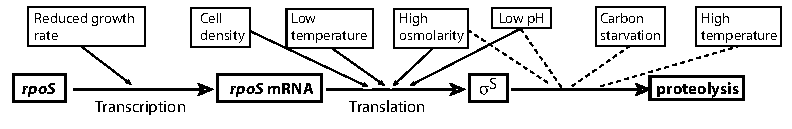
\includegraphics{figures/chap1_rpos_control}
\end{narrow}
\caption[Regulation of \emph{rpoS} expression]{Regulation of
\emph{rpoS} expression by various stressors. The solid arrow
indicates activation and dotted line indicates repression. Redrawn
from \citet{Hengge2002}.} \label{intro_rpos_control}
\end{figure}


\subsection{\emph{rpoS} promoter structure}

In majority of the gram negative bacteria, including \bact{Ec} and
pseudomonads, \emph{rpoS} is always linked with upstream
\emph{nlpD}, coding for a lipoprotein of unknown
function~\citep{Ichikawa1994,Lange1994b}. Downstream of
\emph{rpoS} is variable, even within \bact{Ec}
strains~\citep{Brown2001,Herbelin2000}.

In \bact{Ec}, two independent studies identified three different
transcription start sites of \emph{rpoS} mRNA within \emph{nlpD}
gene~\citep{Lange1995,Takayanagi1994}. Both these studies detected
only one common \e{rpoS} start site within \e{nlpD} (labelled
\e{rpoSp} in Figure~\ref{chap1:rpos_promoter}). This site is now
considered to be the major transcription start site of
\e{rpoS}~\citep{Hengge2002}. Transcription starts with a
T~\citep{Takayanagi1994} or G~\citep{Lange1995} located around
\U{567}{bp} upstream of \e{rpoS} start codon. The $-$10 element
(TATTCT) and $-$35 element (TTGCGT) resemble \siga{} consensus
sequence. These promoter elements are flanked by two cAMP-CRP
binding sites. Although, two upstream \e{nlpD} promoters (marked
\e{nlpDp1} and \e{nlpDp2} in Figure~\ref{chap1:rpos_promoter}) can
contribute to the basal level expression of \e{rpoS} but the
stationary phase expression of \e{rpoS} is solely driven by
\e{rpoSp}~\citep{Lange1995,Takayanagi1994}.

In \e{Pseudomonas}, the start site of the \emph{rpoS} mRNA was
located 366~\citep{Tanaka1994} to 371~\citep{Kojic2002} bases
upstream of the translation initiation codon. The sequences TTGAAT
and TCAATT, separated by 20 bases were found as potential $-35$
and $-10$ promoter elements. An additional observation was the
presence of a binding site of the regulatory protein, \e{psrA}
(see Section~\ref{chap1:psra}) in $-$35 region of the promoters.


\begin{figure}[tbp]
\begin{narrow}{-1in}{-1in}
\centering
\includegraphics{figures/chap1_rpos_promoter}
\end{narrow}
\caption[Distribution of \emph{rpoS} promoters]{Distribution of
\emph{rpoS} promoters.  \emph{rpoSp} is the major \emph{rpoS}
promoter in \emph{E. coli} and the only promoter contributing to
\emph{rpoS} expression in pseudomonads. The position of \e{rpoSp}
in \bact{Ec} (\U{567}{bp} upstream from ATG codon) is different
from the position in pseudomonads (\U{$\sim$370}{bp} upstream from
the ATG codon). Genes are indicated by open arrows showing the
direction. Angled arrows represent the transcription start site.}
\label{chap1:rpos_promoter}
\end{figure}


\subsection{Transcriptional regulation of \emph{rpoS}}

In \bact{Ec}, \emph{rpoS} is mainly regulated by
post-transcriptional mechanism. Although, \e{rpoS} mRNA is present
in high-level, the level of \sigs{} protein is very low during
exponential phase, and mRNA level do not generally change under
stress conditions~\citep{Hengge2002}. Nevertheless, \e{rpoS} mRNA
increases almost five folds during slow growth in rich medium, and
during entry into stationary
phase~\citep{Lange1991,Lange1994,McCann1993,Mulvey1990,Schellhorn1992,Takayanagi1994}.

Several factors have been shown to regulate \e{rpoS}
transcription. Most of the studies had been carried out using
\e{rpoS}::\e{lacZ} transcriptional fusion. A summary of the
presently known key regulators of \e{rpoS} transcription is
presented in Table~\ref{rpos_trans_regulator}.

\begin{table}[tbp]
\linespread{1}\normalsize
\renewcommand{\arraystretch}{1.3}
\begin{minipage}[c]{\textwidth}
\renewcommand{\footnoterule}{}
\renewcommand{\footnotesep}{0pt}
\caption[Regualtors of \e{rpoS} transcription]{Regulators of
\e{rpoS} transcription} \label{rpos_trans_regulator}
\begin{narrow}{-1in}{-1in}
\centering
\begin{small}
\begin{tabularx}{6.1in}{%
@{}>{\raggedright\arraybackslash}p{.9in}%
>{\raggedright\arraybackslash}X%
>{\raggedright\arraybackslash}p{2.5in}%
>{\raggedright\arraybackslash}p{1.9in}@{}}\toprule

\textbf{Regulator} & \textbf{Type}\protect\footnotemark[1] &
\textbf{Observation} & \textbf{Reference}\\\midrule cAMP-CRP &
$+/-$ & \e{rpoS}::\e{lacZ} fusion expression high or low in
different \e{cya} mutant; high in
\e{crp} mutant & \citet{Lange1991,Lange1994,McCann1993}\\
\e{crr} & $-$ & Mutation elevates \e{rpos}::{lacZ} expression
through adenylate cyclase & \cite{Ueguchi2001}\\

Polyamines & $+$ & By stimulating adenylate cyclase expression
which affects RpoS level by positive effect through cAMP-CRP &
\citet{Yoshida2001}\\

GacS-GacA\protect\footnotemark[2] two-component system & $+$ &
Mutations causes more than 80\% reduction in RpoS protein level
and
\e{rpoS}::\e{lacZ} expression & ~\citet{Whistler1998}\\

BarA& $+$ & GacS homolog of \bact{Ec}; mutation decreases \e{rpoS}
mRNA level during exponential phase & \citet{Mukho2000} \\

PsrA\protect\footnotemark[2] & $+$ & A TetR family regulator;
directly induces \e{rpoS} expression binding to its $-$35 element
& \citet{Kojic2001,Kojic2002} \\

Polyphosphate & $+$ & Mutation in \e{ppK}, the gene resposible for
polyphosphate synthesis decreases stationary phase survival;
expression of yeast exopolyphosphatase which depletes
polyphosphate in cell, decreases \e{rpoS}::\e{lacZ} fusion
expression &
\citet{Crooke1994,Rao1996,Shiba1997}\\

ppGpp & $+$ & \e{relA}, \e{spoT} double mutant show reduced level
of \s\smallsu{S}; level can be restored by stimulating ppGpp
accumulation; possibly affect transcriptional elongation rather
than initiation
& \citet{Gentry1993,Lange1995}\\

Quorum sensing molecules & ? & Culture supernatant from spent
growth medium (\e{i.e.}, already grown culture) was used to assay
\e{rpoS}::\e{lacZ} activity. Conflicting data makes it impossible
to draw any conclusion &
\citet{Mulvey1990,Garcia1996,Hengge2002} \\

Weak acids & $+$ & Benzoate increases \e{rpoS}::\e{lacZ}
expression; acetate showed induction in one study, and no effect
in another &
\citep{Mulvey1990,Schellhorn1992}\\

Cellular NADH/NAD\smallsu{$+$} ratio & $-$ & High
NADH/NAD\smallsu{$+$} ratio downregulates \e{rpoS} transcription
& \citet{Sevcik2001}\\

\bottomrule
\end{tabularx}
\end{small}
\end{narrow}
\footnotetext[1]{$+$ and $-$ indicates positive and negative
regulator, respectively. $+$/$-$ indicates both positive and
negative regulator\@. ? indicates no conclusion due to conflicting
reports.} \footnotetext[2]{In pseudomonads.}
\end{minipage}
\linespread{1.1}\normalsize
\renewcommand{\arraystretch}{1}

\end{table}


\subsection{Translational regulation of \emph{rpoS}}

\subsubsection{Regulation by Hfq}

Hfq (HF-I), a \U{11.2}{kDa} RNA-binding protein was first
identified as a host factor essential for phage Q$\betaup$
replication in \e{Ec}. Hfq is highly conserved, very abundant
protein and has been implicated in variety of RNA-mediated
events~\citep{Moller2002,Zhang2002}. There are several
gene-regulatory small RNAs (sRNA) which bind to
Hfq~\citep[reviewed in][]{Wassarman2002}. Interestingly, three of
Hfq binding sRNAs are also involved in \e{rpoS} regulation: OxyS,
DsrA and RprA (see below). Mutation in \e{hfq} has a pleiotropic
phenotype~\citep{Tsui1994}. Hfq stimulates the degradation of
\e{ompA}, \e{miaA}, \e{mutS}, and its own
mRNA~\citep{Tsui1997,Vytvytska1998,Vytvytska2000}. It is also
required for efficient translation of \e{rpoS}
mRNA~\citep{Brown1996,Muffler1996}.

Studies indicated that Hfq probably directly binds to \e{rpoS}
mRNA~\citep{Majdalani2001,Muffler1996b,Sledjeski2001,Zhang1998}. A
5$'$ deletion analysis of \e{rpoS} mRNA indicated that a region
far upstream to the translation initiation site is important for
Hfq action~\citep{Cunning1998}. Mutation in the translation
initiation region of \e{rpoS} mRNA, which potentially disrupts the
secondary structure resulted in increased \e{rpoS} translation and
reduced Hfq dependence~\citep{Brown1997}.

Hfq belongs to a family of proteins including Sm and Lsm, whose
members in higher organism are present in spliceosome and play
important role in mRNA processing~\citep{Moller2002,Zhang2002}.
Consistent to their role in spliceosome, Hfq, in similar manner,
was shown to form ternary complex with its cognate RNA and
regulatory sRNAs. This complex formation was demonstrated at least
in two cases: OxyS binding with \e{flhA} mRNA and Spot42 with
\e{galK} mRNA~\citep{Moller2002,Zhang2002}. It was, therefore,
proposed that Hfq might control \e{rpoS} activity in a similar
manner~\citep{Wassarman2002,Hengge2002}.

\subsubsection{Regulation by H-NS}

H-NS is an abundant histone-like protein shown to form
nucleoprotein complexes and acts as a repressor for a variety of
genes. StpA is a paralog of H-NS, which acts more as an RNA
chaperone. Both H-NS and StpA are known to form homo- and
hetero-oligomers~\citep[reviewed
in][]{Atlung1997,Dorman1999,Williams1997}. H-NS is also known to
be a cold-shock protein~\citep{Teana1991}.

H-NS mutant exhibits strongly increased RpoS level at all growth
stages \citep{Barth1995,Yamashino1995}, due to enhanced
translation of \e{rpoS} mRNA and suppression of RpoS
proteolysis~\citep{Yamashino1995}. The molecular mechanism of H-NS
mediated repression of RpoS expression is still unclear, but may
be indirect, as H-NS deficiency has no effect on \e{rpoS}
translation in \e{hfq} mutant background~\citep{Muffler1996}.
DsrA, a regulatory sRNA (see below) is also known to suppress
H-NS~\citep{Lease2000}. H-NS is also known to play an antagonistic
role with HU, another known regulator of
\e{rpoS}~\citep{Dri1992,Deighan2000,Painbeni1997}. It might also
be possible that H-NS modulates \e{rpoS} by affecting
HU~\citep{Hengge2002}.

\subsubsection{Regulation by HU}

HU is a major component of the bacterial nucleoid and also
participates in gene regulation, DNA recombination, and DNA
repair~\citep{Hengge2002}. Moreover, HU is required for optimum
survival during prolonged starvation \citep{Claret1997}. In
Enterobacteriaceae and Vibrionaceae, two subunits, HU$\alphaup$
and HU$\betaup$, encoded by \e{hupA} and \e{hupB}, respectively,
contribute to the formation of active HU
protein~\citep{Oberto2001}\@. \e{hupAB} mutant exhibits strongly
reduced RpoS level due to reduced translation of \e{rpoS}
mRNA~\citep{Balandina2001}. HU binds with high affinity to a 150
nucleotide fragment of \e{rpoS} mRNA spanning the translation
initiation region~\citep{Balandina2001}.

\subsubsection{Riboregulators in RpoS expression}
\label{chap1:srna} Recently, it is becoming clearer that
abundantly present small regulatory RNAs (sRNA) play a very vital
role in gene regulation~\citep[reviewed
in][]{Altuvia2000,Wassarman2002,Eddy2001}. Collectively termed as
\e{riboregulators}, three of these sRNAs had already been found to
have profound influence on \e{rpoS} expression. DsrA and RprA
promote \e{rpoS} translation and OxyS inhibits it. All these sRNAs
are known to bind to Hfq~\citep{Wassarman2002}.

DsrA was originally identified as a multicopy suppressor of
H-NS-mediated silencing of \e{rcsA} gene in
\bact{Ec}~\citep{Sledjeski1995} and later on found to be essential
for increased \e{rpoS} translation at low
temperature~\citep{Sledjeski1996}.

DsrA is a 87 nucleotide RNA that folds into a three stem-loop
structure~\citep[][Figure~\ref{chap1_dsra}]{Lease2000,Majdalani1998}.
The stem-loop 1 and the following single-stranded part of DsrA
(marked with solid line in Figure~\ref{chap1_dsra}) are
complementary to an upstream \e{antisense element} of \e{rpoS}
mRNA that is assumed to base pair with the translation initiation
region (see also Chapter 4). This suggests that DsrA functions by
an \e{anti-anti-sense} mechanism that disrupts the intramolecular
basepairing  in \e{rpoS}
mRNA~\citep{Lease2000,Lease1998,Majdalani1998,Lease2000b}. DsrA
plays only a minor role in \e{rpoS} translation in cells growing
at higher temperature, but becomes a major stimulating factor at
low temperature~\citep{Sledjeski1996}. This stimulation is due to
increased transcription of \e{dsrA}, and a six fold increase in
the stability of DsrA at low temperature~\citep{Repoila2001}. Hfq
stabilizes DsrA, as well as alters its secondary structure to
enable it to interact with \e{rpoS} mRNA~\citep{Sledjeski2001}.


\begin{figure}[tbp]
\centering
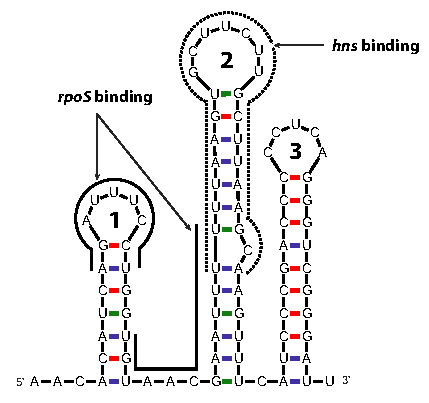
\includegraphics{figures/chap1_dsra}
\caption[DsrA sturcture]{DsrA RNA secondary structure. The lowest
energy structure predicted by MFOLD version
3.1~\citep{Mathews1999} is shown. The putative regions of \e{rpoS}
(solid line) and \e{hns} (dotted line) binding sites are
labelled.} \label{chap1_dsra}
\end{figure}

Besides directly regulating \e{rpoS}, DsrA negatively regulate
\e{hns} mRNA by formation of a coaxial stack with two regions of
\e{hns} mRNA by its unfolded stem-loop region 2
(Figure~\ref{chap1_dsra})\@. The \e{hns} mRNA is more efficiently
degraded within this complex~\citep{Lease2000b}. In what seems
like a reciprocal suppression, StpA and H-NS also represses
DsrA~\citep{Lease2000b}.

An indirect regulation of \e{rpoS} is also brought about by LeuO,
a LysR like regulator that binds to \e{dsrA}
promoter~\citep{Repoila2001} and represses its expression.
Overproduction of LeuO reduces \e{rpoS} translation in
DsrA-dependant manner particularly at low
temperature~\citep{Klauck1997}.

OxyS, a 109 nucleotide sRNA, which is induced by oxidative stress,
acts as a pleiotropic regulator~\citep{Altuvia1997}. A single
stranded A-rich region in OxyS RNA with no apparent sequence
complementarity with \e{rpoS}, is involved in the negative
regulation of \e{rpoS} translation~\citep{Zhang1998}. OxyS
coimmunoprecipitates Hfq, thus indicating that it might form a
translationally incompetent ternary complex with
\e{rpoS}~\citep{Zhang1998}.

Another sRNA involved in \e{rpoS} regulation is RprA, which was
identified as a multicopy suppressor for \e{dsrA}
mutation~\citep{Majdalani2001}. In presence of DsrA, neither
overproduction nor knockout of RprA has any effect on \e{rpoS}
expression.

\subsubsection{Other regulators}

There are several other regulators that have been shown to affect
RpoS expression at the level of translation. These regulators are
briefly described below.

\begin{description}

\item[\textbf{dnaK}] is a heat-shock chaperone\@. \e{dnaK} mutant
exhibits reduced \sigs{} level due to reduced \e{rpoS}
translation~\citep{Muffler1997,Rockabrand1998}.

\item[\textbf{DksA}] is zinc-binding protein. \e{dksA} mutation in
\e{Salmonella} exhibit reduced \sigs{} expression at stationary
phase and after a shift to acidic pH~\citep{Webb1999}.

\item[\textbf{EIIA(Glc)}] is negative regulator of \e{rpoS}
translation\@. In \e{crr} mutant which is defective in EIIA(Glc)
contains strongly elevated \sigs{}, which is suppressed by
external addition of cAMP~\citep{Ueguchi2001}.

\item[\textbf{CspC and CspE}] belongs to the cold shock protein
family in \bact{Ec}, although they are not cold-inducible.
Overproduction of these two RNA binding protein stabilizes
\e{rpoS} mRNA~\citep{Phadtare2001}.

\item[\textbf{UDP-glucose}] deficiency caused by mutation in
carbon-metabolism genes exhibits increased \sigs{} level during
exponential growth~\citep{Bohringer1995}.

\end{description}



\subsection{Control of \emph{rpoS} proteolysis}
\label{chap1_rssb}

In \bact{Ec}, \sigs{} level is low during exponential growth phase
due to its rapid degradation. Under stress conditions, the
proteolysis is prevented very quickly~\citep{Lange1994}. The
proteolysis is mediated by ATP-dependant ClpXP protease. Mutation
in the \e{clpP} and \e{clpX} results in stabilization of \sigs{}
\citep{Schweder1996}.

ClpXP can not degrade the \sigs{} alone. For this it requires a
recognition factor called RssB(SprE, MviA, ExpM in different
bacteria)~\citep{Muffler1996c,Hengge2002}. A mutation in \e{rssB}
stabilizes \sigs{}, resulting in elevated expression in
exponential phase~\citep{Muffler1996c}.

RssB is a response regulator of a two component pathway whose
cognate sensor kinase is yet unidentified. Acetyl phosphate is
known to play a role in RssB phosphorylation~\citep{Bouche1998}.
It is phosphorylated at its N-terminal domain at a conserved
aspartyl residue (D58)~\citep{Becker1999}. The phosphorylated form
directly binds to \sigs{} in equimolar ratio~\citep{Klauck2001}.
The binding involves K173 in region 2.5 of \sigs{}. A single point
mutation K173E was shown to stabilize \sigs{}~\citep{Becker1999}.
Once formed, the RssB-\sigs{} complex is recognized by ClpXP
protease and the \sigs{} is completely degraded in an
ATP-dependant manner.


\section{\emph{rpoS} in pseudomonads}
\index{rpoS@\emph{rpoS}!in pseudomonads}

A \emph{rpoS} homolog was cloned from Pseudomonads for the first
time in 1994, from \emph{P. aeruginosa}~\citep{Tanaka1994}. The
operon structure of \e{rpoS} was found to be similar to that of
\emph{E. coli}. The RpoS level was found to be higher at the onset
of stationary phase and the gene could restore the catalase
activity in \emph{rpoS}-deficient strain of \bact{Ec}. Strangely,
the same group in another article reported the inability of \emph{
P. aeruginosa rpoS} to get transcribed in \emph{E.
coli}~\citep{Fujita1994}. \emph{rpoS} was found to be transcribed
from its own promoter and the start site of the \emph{rpoS} mRNA
was located 366 bases upstream of translation initiation codon.
The sequences TTGAAT and TCAATT, separated by 20 bases were
identified as $-35$ and $-10$ elements of potential promoter. The
downstream region of the $-10$ sequence (GGGCCAGC) was found to be
similar to the ``gearbox'' sequence (CGGCAAGT).

Other studies on \emph{P. aeruginosa rpoS} indicated its role in
stationary-phase-specific stress resistance~\citep{Jorgensen1999}.
Interestingly, at stationary-phase \emph{rpoS}$^{-}$ cells were
much more stress resistant than \emph{rpoS}$^{+}$ cells from
exponential phase. Studies on \emph{P. aeruginosa} PAO1 also
showed that \emph{rpoS}$^{-}$ cells were sensitive to carbon
starvation only in medium containing glucose as carbon
source~\citep{Suh1999}. In addition, the \emph{rpoS} mutant of
PAO1 was hypersensitive to heat shock at 50\dg, increased
osmolarity, and prolonged exposure to high concentrations of
H$_{2}$O$_{2}$. Catalase production was also 60\% lower in these
mutants. The rpoS mutant produced 50\% less exotoxin A, but
produced only slightly smaller amounts of elastase and LasA
protease than the parent strain. The levels of phospholipase C and
casein-degrading proteases were also unaffected by a mutation in
\emph{rpoS} in PAO1. The rpoS mutation resulted in the increased
production of the phenazine antibiotic pyocyanin and the
siderophore pyoverdine. In an alginate-overproducing cystic
fibrosis (CF) isolate, FRD1, the \emph{rpoS101::aacCI} mutation
almost completely abolished the production of alginate when the
bacterium was grown in a liquid medium. On a solid medium, the
FRD1 \emph{rpoS} mutant produced approximately 70\% less alginate
than did the wild-type strain. Two cytotoxic lectins, PA-IL and
PA-IIL in PAO1 were also found to be controlled by
\emph{rpoS}~\citep{Winzer2000}.

Second \emph{rpoS} from \emph{Pseudomonas} sp. was isolated and
characterized from \emph{P. fluorescens}
\mbox{Pf-5}~\citep{Sarniguet1995}. The production of the
antibiotic pyrrolnitrin was found to be \emph{rpoS}-dependent. The
\emph{rpoS} in \e{P. fluorescens} was also found to make the cells
resistant to high-salt and hydrogen peroxide, and influenced the
survival of the bacteria on plant.


\emph{rpoS} from \emph{P. putida} were cloned from strain
KT2440~\citep{Ramos1998} and WCS358~\citep{Kojic1999}. The
\emph{rpoS} from this strain could complement the acid-sensitivity
and catalase deficiency of \emph{E. coli rpoS}-mutant, and could
drive the expression from \emph{bolA$_{p1}$} promoter. The
\emph{rpoS} mutant of KT2440 showed reduced survival under carbon
starvation and ethanol-stress. \e{rpoS} in this strain could
control at least 50 proteins which were expressed under carbon
starvation. The \e{rpoS} gene was also characterized from a WCS385
strain of \emph{P. putida}, which is a rhizosphere-colonizing
plant growth-promoting bacterium. \emph{rpoS} from this strain was
found not to be involved in siderophore or homoserine lactone
production.


\subsection{GacS and GacA controls RpoS in pseudomonads}

In \emph{P. fluorescens},  the production of antifungal metabolite
is controlled by two-component regulatory system comprised of GacS
and GacA. \emph{gacA} encodes response regulator of FixJ family
and \emph{gacS} encodes the cognate sensor kinase. Recently, it
has been shown that GacA controls the expression of a small
regulatory RNA, \emph{rsmZ} which by titration effect on another
protein RsmA controls expression of several secondary metabolites
production~\citep{Heeb2002}. GacA and GacS are present in various
species of \emph{Pseudomonas}~\citep{Kitten1998}. It was found
that the RpoS content in \emph{gacS} and \emph{gacA} mutants of
\emph{P. fluorescens} Pf-5 was less than 20\% of the wild-type
level~\citep{Whistler1998}.

\subsection{\emph{rpoS} in quorum sensing}

\emph{lasR}, the \emph{luxR} homolog in \emph{P. aeruginosa},
constitutively expressed throughout the growth cycle, together
with $N$-(3-oxododecanoyl)-$L$-homoserine lactone (OdDHL) that
controls \emph{rhlR} expression and rhamnolipid production in
stationary phase. Interestingly, the expression of \emph{rpoS} is
abolished in \emph{lasR} mutant and $N$-butanoyl-$L$-homoserine
lactone (BHL) mutant of \bact{Pa}, PANO67~\citep{Latifi1996}. As
suggested by this study that \emph{rpoS} transcription is directly
controlled by RhlR and RhII (involved in BHL production). In
another study it was shown that in \emph{rpoS} mutant, there was
an increase in the production of RhII but not RhlR, which resulted
in higher level of acylhomoserine lactone
production~\citep{Whiteley2000}. The connection of quorum sensing
mechanism with stringent response was established by the fact that
\emph{relA} overproduction resulted in premature induction of
\emph{lasR} and \emph{rhlR}. This expression was found to be
independent of \emph{rpoS}. \emph{relA} overexpression also caused
activation of \emph{rpoS} and the consequent cell-density
independent expression of \emph{lasB} elastase, a virulence factor
in \emph{P. aeruginosa} PAO1~\citep{Delden2001}.

\subsection{\emph{rpoS} regulation by TetR family member PsrA}
\label{chap1:psra}

PsrA (\emph{Pseudomonas} sigma regulator), a protein of
\U{26.3}{kDa} was found to be involved in stationary-phase-induced
transcriptional regulation of \emph{rpoS} in \emph{P. putida}
WCS358 and also in \emph{P. aeruginosa}~\citep{Kojic2001,
Kojic2002}. Inactivation of \emph{psrA} caused 90\% reduction of
\emph{rpoS} promoter activity~\citep{Kojic2001}. PsrA mutants were
twofold more sensitive to high temperature (50\dg{}) and high-salt
than the parent strain. RpoS protein level was also found reduced
to almost half in the mutant than that of parent strain. PsrA on
the other hand played no role in the production of homoserine
lactone. PsrA was also found to control negatively its own
promoter. In a later report, PsrA was found to bind directly to
the \emph{rpoS} promoter to a palindromic sequence covering $-$59
to $-$35 (TTGCTTCAAACGGTAGTTTGAATAA) with respect to $+$1
transcription start site. Comparing the binding sites in
\emph{rpoS} of \emph{P. putida} WCS358 and \emph{psrA} the
consensus was derived as {\small\texttt{G/CAAACN$_{2-4}$GTTTG/C}}
\citep{Kojic2002}. In addition, \emph{psrA} was found to express
more during the entry of the cells to stationary phase and
induction is more in cells lacking \emph{psrA}.

\subsection{Presence of Hfq in \emph{P. aeruginosa}}

As described earlier, Hfq protein is required for \emph{rpoS}
translation in \emph{E. coli} and \emph{S. typhimurium}. A Hfq
homolog of \emph{P. aeruginosa} which consists of only \U{82}{aa}
has recently been cloned~\citep{Sonn2002}. The 68 amino acids at
the N-terminal end of Hfq homolog of \emph{P. aeruginosa}
exhibited 92\% identity with Hfq of \emph{E. coli}. The \emph{P.
aeruginosa} homolog could also functionally complement \emph{E.
coli}, in terms of its requirement for phage Q$\beta$ replication
and for \emph{rpoS} expression~\citep{Sonn2002}. The presence of
Hfq in \emph{P. aeruginosa} indicated that it might also be
involved in regulating \emph{rpoS} expression in this bacterium.

\section{Mutability of the \e{rpoS}}
\label{chap1:rpos_mutation}

It has now been established that \e{rpoS} in laboratory strains
and natural isolates of \bact{Ec} and \e{Salmonella}, tend to
accumulate mutations
\citep{Jishage1997,Ivanova1992,Visick1997,Atlung2002,Jorgensen2000,Sutton2000}.
There are several different types of mutations accumulate in
\e{rpoS}, but amber mutation is very common in many of these
strains. In many of these amber-mutated \e{rpoS} strains, \e{rpoS}
expression is not probably affected due to amber
suppressors~\citep{Rod1988}. These strains show variability in
\e{rpoS}-dependent phenotypes such as,
acid-sensitivity~\citep{Waterman1996} and resistance to
hydrostatic pressure~\citep{Robey2001}. The significance of the
occurrence of such mutations in \e{rpoS} is still not well
understood.


\section{GASP mutants}
\label{chap1:gasp} Prolonged incubation of batch cultures of
\bact{Ec} results in the loss of viability~\citep[reviewed
in][]{Huisman1996,Finkel1998}. A fraction of cells, however,
survives, and are able to form colonies even after a year. When
mixed in very low ratio with freshly grown stationary phase cells
(1:10,000), these survivors dominate the culture by outcompeting
other cells. This growth advantage of the survivors was found to
be due to the accumulation of mutations~\citep{Zambrano1993},
expressing \e{G}rowth \e{A}dvantage at \e{S}tationary \e{P}hase
(GASP) phenotype, characterized by the ability to grow, when the
ancestral population can not. The GASP mutants, apparently, grow
by scavenging nutrients from the dying cells~\citep{Zinser1999}.
Multiple rounds of mutants arise to take over the culture during
prolonged starvation~\citep{Finkel1999}. Interestingly, the first
round of mutation are always in \e{rpoS} gene~\citep{Vulic2001}.
The first GASP allele of \e{rpoS} was identified to contain a
small duplication near the 3$'$ end of the gene, resulting in a
frame-shift which replaced the last four residues with 39 new
amino acids~\citep{Zambrano1993}. All the GASP mutants identified
so far exhibits reduced activity of \e{rpoS}, but are not
\e{rpoS}-null. This suggests that reduction, not the elimination
of \e{rpoS} activity, is required to express the GASP
phenotype~\citep{Finkel1998}.

The growth advantage of the GASP mutants have been explained in
terms of \e{prisoner's dilemma} in game
theory~\citep{Axelrod1981,Vulic2001}. In prisoner's dilemma, two
players each has two options, to cooperate or not to cooperate
(defect). If both cooperate, they receive a reward, \e{R}, which
is larger than the punishment, \e{P}, obtained if both defect. If
one defects and the other cooperates, the defector obtains a
pay-off, \e{T} (the temptation), which is greater than the \e{R},
and the cooperator receives the sucker's payoff, \e{S}, which is
less than \e{P} (\e{T}>\e{R}>\e{P}>\e{S}). Because, under this
situation, regardless of opponent's strategy it always pays off to
defect, both the players will end up in
defecting~\citep{Axelrod1981}. GASP mutants in the present case,
acts as a defector, whereas, the dying wild type cells conforms
(cooperators) in maintaining the stationary phase. Because of the
defect in \e{rpoS}, GASP mutants avoid the growth inhibition
during stationary phase at the cost of the wild type cells. This
phenomenon has been termed as \e{evolutionary
cheating}~\citep{Vulic2001}. \citet{Vulic2001} also calculated the
fitness values (T,R,P, and S) which conforms largely to the order
required for supporting \e{prisoner's dilemma}.

\mathversion{bold}
\section{\s{} factor competition model}
\mathversion{normal}
\label{chap1:compete}

As discussed in the earlier Sections, there are multiple
$\sigmaup$ factors in a cell. Each of them directs transcription
from a specific set of promoters during growth. It has been
estimated that in \bact{Ec} and probably in other bacteria, the
total number of core RNA polymerase (600--700 molecules),
available for binding by \s{} is far less the total number of \s{}
($\sim$1200) molecules~\citep{Ishihama2000}. This creates a
competition among the \s{} factors to bind to the core enzyme.
This model, referred to as \s{} factor competition model is also
supported by the fact that lowering the level of one \s{} factor,
upregulates the activity of the
other~\citep{Farewell1998,Zhou1992}. As will be revealed in this
study, this phenomenon probably plays a very vital role in the
cold adaptation of Lz4W\@. The following is a brief account of the
model with special emphasis on the major \s{} factor, \s\su{D} and
stress responsive \s{} factor, \s\su{S}.

The first factor that determines the \s{} binding to the core is,
of course, the expression level of each \s{} factor. It has been
estimated in \bact{Ec} that the core enzyme level remains constant
throughout the growth stages~\citep{Ishihama2000}. The
concentration of \siga{} is highest among all the \s{} factors in
both exponential and stationary phase and under various stress
conditions~\citep{Jishage1995,Jishage1996}. \siga{} also has the
highest affinity to the core (K\sub{m} \U{0.26}{nM}), while
\sigs{} has the weakest binding affinity (K\sub{m}
\U{4.28}{nM})~\citep{Ishihama2000}.

How does then \sigs{} can transcribe at all? There are several
mechanisms by which \sigs{} competes with \siga{}. One of the
mechanisms is through anti-\s{} factor~\citep[reviewed
in][]{Hughes1998}. An anti-\s{} factor is defined by its ability
to form a complex with its cognate \s{}, thereby inhibiting its
binding to core RNAP\@. The control of \s{} by anti-\s{} has been
well established in \e{B. subtilis}~\citep{Kroos1999,Brown1995}.
Among seven \s{} subunits of \bact{Ec}, anti-\s{} has been
identified for \siga{}, \s\su{F} and \s\su{E}, called, Rsd, FlgM,
RseE, respectively \citep{Jishage1998,Jishage1999,Kut1994,De1997}.
Interestingly, the anti-\s{} factor of \siga{}, Rsd, is
upregulated at stationary phase and is under \sigs{}
control~\citep{Jishage1999}. Evidences are accumulating about two
other factors that increase the affinity of \sigs{} to core RNAP:
first, the \e{alarmone} ppGpp~\citep{Jishage2002}; second, 6S
RNA~\citep{Wassarman2000}. All these mechanisms together
contribute to make \sigs{} transcribe from specific promoters in
spite of the presence of a large molar excess of \siga{}.




\mathversion{bold}
\section{Role of \s{} factor in cold adaptation}
\mathversion{normal}

Unlike the heat-shock response in bacteria, where involvement of a
specific \s{} factor (\s\su{H} in Gram-negative bacteria) has been
directly proved, no such cold-shock \s{} factor has been
identified till date. This perhaps indicates the complexity of the
low temperature adaptation. However, there are two reports
implicating \s\su{E} in a deep-sea psychrophile \e{Photobacterium}
sp.~\citep{Chi1995} and \e{sigB} in psychrotroph \e{Listeria
monocytogenes}~\citep{Becker2000} to growth at low temperature.

The role of \e{rpoS} in cold adaptation, however, remains arguable
at its best. In \bact{Ec}, \sigs{} level is shown to be
upregulated during growth at low temperature. \e{rpoS} mutant,
however, has no growth defect during growth at low
temperature~\citep{Sledjeski1996}.

\section{The objectives of the present study}
The above discussion highlights the various aspects of
cold-adaptation and the importance of transcription in the gene
regulation at lower temperature. It is apparent that almost no
information exists on the mechanism of transcription and the role
of \s{} factors during transcription at low temperature, which is
crucial for the growth and survival for the Antarctic \e{P.
syringae} Lz4W. The objectives of the present study, therefore,
were:

\begin{enumerate}

\item To clone and analyze the \e{rpoD} and \e{rpoS} genes coding
for the primary \s{} factor, \s\su{D} and stationary phase \s{}
factor, \sigs{} of \e{P. syringae} Lz4W.

\item To investigate the role, if any, of the stationary phase,
and stress responsive, \sigs{} subunit of RNA polymerase in
cold-adaptation and the associated stress response of \e{P.
syringae} Lz4W.

\item To compare the cloned \s{} genes with their mesophilic
counterpart to gain a possible insight into the modifications that
these genes might have undergone during adaption to low
temperature.\ding{45}

\end{enumerate}


\FloatBarrier\pagebreak \thispagestyle{empty}
\begin{figure}[h]
\raggedleft
\includegraphics{figures/chap2_sep}
\end{figure}
\thispagestyle{empty}

\chapter{Materials and Methods}
%\minitoc

\section{Chemicals}

Agarose, ethidium bromide, X-gal, IPTG, SDS, BSA, acrylamide,
bis-acry\-la\-mide, $\betaup$-mercapto\-ethanol, ammonium
persulphate, TEMED, Tris, EDTA, and MOPS were procured from
various vendors including Gibco-BRL, Sigma, Calbiochem and others.
Tryptone, yeast extract, peptone and agar powder for preparation
of culture media were obtained from Hi Media (India). All
restriction enzymes, Klenow polymerase, T4 DNA ligase, and
polynucleotide kinase were purchased from New England Biolabs Inc.
(USA). Lysozyme, DNase I, RNase, Proteinase K were purchased from
Roche (Germany). \textit{Taq} DNA polymerase, DNA and protein
molecular weight markers were purchased from Bangalore Genei
(India). DNA and RNA purifying kits were purchased from QIAGEN and
Promega. Phage packaging kit was from Stratagene (USA). The DNA
random primer kit for labelling DNA, and radiolabelled nucleotides
were from BRIT (India). Sephadex G-50 and G-25 were from Pharmacia
Bio\-tech (Sweden). Custom made oligonucleotides were obtained
either from Oswel (UK) or from in-house oligo synthesis facility.
Nitrocellulose, Hybond{\scriptsize\texttrademark}-N\su{+} and
PVDF{\scriptsize\texttrademark} membranes were from Amersham (UK)
and Whatman filter paper from Whatman International ltd. (USA).
X-ray films were obtained from Konica Corporation (Japan). All
other chemicals were purchased from local manufacturers and were
of analytical grade.

\section{Software} All sequence analyses were performed over WWW
using SeWeR~\citep{Basu2001} interface. In some special cases,
custom-made Perl scripts were used. Other specific softwares are
mentioned in this text as and when required.

\section{Oligonucleotides}

The oligonucleotides used in this study are listed in
Table~\ref{chap2_oligos}.

\begin{table}[tbp]
\linespread{1}\normalsize
\renewcommand{\arraystretch}{1.5}
\begin{minipage}[c]{\textwidth}
\renewcommand{\footnoterule}{}
\caption{Oligonucleotides used in this study} \label{chap2_oligos}
\begin{narrow}{-1in}{-1in}
\centering
\begin{small}
\begin{tabular}{@{}lp{4.5in}@{}}\toprule
\textbf{Name} & \textbf{Sequence\protect\footnote{From 5$'$ to
3$'$ direction.}}\\\midrule ``\emph{rpoD} box'' (Probe1) &
GCTTGGCGGATCCACCAGGTGGCGTAGGT\\
``\emph{rpoD} box'' (Probe2) &
GCTTGICIIATCCACCAIGTIGCITAIGT\protect\footnote{I stands for inosine.}\\
RPODFP1 &
AAGTTCTC(G/A/T/C)AC(C/G)TA(T/C)GC(A/T/G/C)ACC(G)T\-G\-G\-T\-G\-G\-A\-T\\
RPODFP2 & AAGTTCTC(C/G)ACCTACGC(A/C)ACCTGGTGGAT \\
RPODRP1 &
GCCTT(C/G)GCTTC(G/A)AT(C/T)TG(G/C/A/T)CG(G/A)\-AT\-(A/C/G/T)\-C\-(G/T)(C/T)TC\\
RPODRP2 &
GCCTT(C/G)GC(C/T)TCGATCTG(A/G)CGGAT(A/C)CG(C/T)TC\\
RPOSKOF &
CCG\textbf{\underline{GAATTC}}CTACTACTGCCCGCACCAAGT\protect\footnote{\emph{Eco}RI
site indicated in boldface and underlined.} \\
RPOSKOR &
CCC\textbf{\underline{AAGCTT}}AAAAGCATGCGCTTGACCTC\protect\footnote{\emph{Hin}dIII
site indicated in boldface and underlined.}\\
\bottomrule
\end{tabular}
\end{small}
\end{narrow}
\end{minipage}
\linespread{1.1}\normalsize
\renewcommand{\arraystretch}{1.0}
\end{table}
\section{Plasmids and cosmid}

\begin{description}

    \item [\textbf{pBluescriptII KS+}] (Stratagene) is a high-copy-number, ColE1-based
    vec\-tor, which confers ampicillin resistance (Amp\su{r}) to the host cell.
It also carries a
        multiple cloning site region in \textit{lacZ$\alphaup$}
        fragment enabling blue-white screening of the recombinant
        clone.
    \item[\textbf{pUC19}] (Pharmacia) is a high-copy-number, ColE1-based vector containing Amp\su{r} marker, and carries
    \textit{lacZ}$\alphaup$ fragment enabling blue-white screening
    of the recombinant clone.

    \item [\textbf{pDB18R}] \citep{Fujita1994} is a high-copy-number plasmid
        construct derived from pTZ18R (Pharmacia). It carries a
        \unit[1.8]{kb} \textit{Kpn}I-\textit{Hind}III fragment containing
        \bact{Pa} \textit{rpoS} promoter and
        structural gene.

    \item [\textbf{pASB3}] \citep{Tanaka1991} is plasmid pTZ18R carrying a
        \unit[2.3]{kb} \textit{Pst}I DNA fragment containing \textit{rpoD} of
        \bact{Pa}.

    \item [\textbf{pLAFR3}] \citep{Staskawicz1987} is a broad-host-range cosmid with Tc\su{r} marker; allows blue-white screening because of the presence of
\emph{lacZ}$\alphaup$ fragment.

    \item [\textbf{pGEMD}] \citep{Igarashi1991} is derived from
    pGEMEX1 (Promega) containing a \U{2.1}{kb} \emph{Hin}dIII
    fragment spanning the full-length \emph{rpoD} of \bact{Ec}.

    \item[\textbf{pGEMAX185}] \citep{Igarashi1991} is derived from
    pGEMEX1 (Pro\-mega) containing \U{1.2}{kb} \emph{Xba}I
    fragment spanning the full-length \emph{rpoA}
    of \emph{E. coli}.

    \item[\textbf{pGEMBC}] \citep{Igarashi1991} is derived from
    pGEMEX1 (Promega) containing a \U{10.2}{kb} \emph{Hin}dIII
    fragment spanning the full-length \emph{rpoB}, and \emph{rpoC}
    gene of \emph{E. coli} with upstream \emph{rplL}.

    \item[\textbf{PGEM-T}] (Promega) is a TA cloning vector of size \U{3003}{bp}, and is used to clone
    PCR product with A-overhang. It contains Amp\su{r} marker and
    \textit{lacZ}$\alphaup$ for screening of recombinant clones.

    \item[\textbf{pCL1920}] \citep{Lerner1990} is a low-copy-number
    vector with pSC101 replicon ($\sim$5 copies/cell). It
    carries streptomycin/spectinomycin resistance mar\-ker (encoded
    by \emph{aadA}), and also carries \emph{lacZ}$\alphaup$ that
    allows blue-white screening of the recombinants.

    \item[\textbf{p4A4}] is pBluescriptII KS$+$ containing a
    \emph{Sal}I--\emph{Pst}I insert of \U{$\sim$2}{kb} containing C-terminal half of \emph{rpoD} homolog of \emph{P.
    syringae} (Lz4W).

    \item[\textbf{p4C12}] is pBluescriptII KS+ containing a
    \U{$\sim$2.1}{kb} \emph{Pst}I fragment with the
    full-length \emph{rpoS} of \emph{P. syringae} (Lz4W).

    \item[\textbf{pRPOH5}] \citep{Aramaki1996} is plasmid pTZ18R containing a
    \U{1.9}{kb} \emph{Sal}I--\emph{Pst}I fragment spanning the
    full-length \emph{rpoH} of \bact{Pa}.

    \item[\textbf{pGL10}] \citep{Bidle1999} is a broad-host-range
    cloning vector with IncP replicon. It has a genotype,
    \emph{tra}\su{$-$} \emph{mob}\su{$+$} and Km\su{r}.

    \item[\textbf{pGLSIGS}] is pGL10 containing the insert of
    p4C12.

    \item[\textbf{pXRPOS}] is pGL10 containing
    \emph{Pst}I--\emph{Bam}HI fragment from p4C12 and
    \emph{Bam}HI--\emph{Hin}dIII fragment from pDB18R, ligated in
    tandem, which results in a chimeric \emph{rpoS}.

    \item[\textbf{pME3088}] \citep{Schnider2000} is a suicide vector with ColE1 replicon with genotype,
    \emph{RK2-Mob} Tc\su{r}.

    \item[\textbf{pMERPOS$'$}] is pME3088 containing a
    \U{$\sim$750}{bp} internal fragment of \emph{rpoS} gene of
    Lz4W.


\end{description}




\section{Culture media}

All media were prepared using water purified through MilliQ water
purification system (Millipore).

\begin{longtable}{lll}\addlinespace
\multicolumn{3}{@{}l}{\textbf{1. Culture media for \bact{Ps}
(Lz4W)}}\\\addlinespace
\multicolumn{3}{l}{\textbf{Antractic Bacteria Medium (ABM) broth:}}\\
    &   Peptone &  \unit[5]{g} \\
    & Yeast extract & \unit[2.5]{g} \\
       & Water to   &    \unit[1000]{ml}\\
       &     \multicolumn{2}{l}{pH adjusted to 7.0-7.2 with \unit[1]{M} NaOH.}\\
       &     \multicolumn{2}{l}{Sterilized by autoclaving.}\\
       \addlinespace

{\bfseries ABM agar:} & ABM  &  \ml{100}\\
              &  Agar & \U{1.5}{g}\\
              \addlinespace\midrule\addlinespace

\multicolumn{3}{@{}l}{\textbf{2. Culture media for
\bact{Ec}}}\\\addlinespace
{\bfseries LB medium:} &  Tryptone & \unit[10]{g} \\
                        & Yeast extract & \unit[5]{g}\\
                       & NaCl  &  \unit[10]{g}\\
                & Water to & \unit[1000]{ml}\\
    &     \multicolumn{2}{l}{pH adjusted to 7.0-7.2 with \unit[1]{M} NaOH.}\\
       &     \multicolumn{2}{l}{Sterilized by
       autoclaving.}\\\addlinespace

    {\bfseries LB agar:} &   \multicolumn{2}{l}{LB medium with 1.5\%
    (\nicefrac{w}{v}) agar.}\\\addlinespace


    {\bfseries LB soft agar:} & \multicolumn{2}{l}{LB medium with 0.6\% (\nicefrac{w}{v}) agar.}\\\addlinespace

    \textbf{SOB medium:} & Tryptone  & \U{20}{g} \\
                        & Yeast extract & \U{5}{g}\\
                        & NaCl          & \U{0.5}{g}\\
                        & Water to      &\ml{1000} \\
                        & \multicolumn{2}{p{3in}}{pH adjusted to 7. Sterilized by autoclaving, and just before use, \ml{5} of sterile \U{2}{M} MgCl\sub{2} was added.}\\\addlinespace

    \textbf{SOC medium:} & SOB medium  & \ml{1000} \\
                        & Glucose (\U{1}{M}) & \ml{20}
                        \\\addlinespace

    {\bfseries Z broth:} & \multicolumn{2}{l}{LB medium supplemented with 0.5\% (\nicefrac{v}{v}) CaCl\sub{2}
    (\U{0.5}{M}).}\\\addlinespace

    {\bfseries Z agar:} & \multicolumn{2}{l}{Z broth with 0.75\%
    (\nicefrac{w}{v}) agar.}
    \addtocounter{table}{-1}
\end{longtable}

\section{Buffers and solutions}
    \label{buffers}
    \begin{longtable}{llll}
   \multicolumn{4}{@{}l}{\textbf{1. Plasmid isolation solution for alkaline
    lysis}}\\\addlinespace
  &\textbf{Solution 1:} &  Glucose & \mM{50}\\
  &                     &  Tris-Cl (pH 8.0) & \mM{25}\\
   &                & EDTA (pH 8.0) & \mM{10}\\\addlinespace
   & \textbf{Solution 2:} & NaOH &   \U{0.2}{M} \\
    &                   &  SDS & 1\% \\\addlinespace
    &\textbf{Solution 3:} & Potassium acetate (\U{5}{M}) & \ml{60}\\
    &                 & Glacial acetic acid & \ml{11.5}\\
     &                & Water & \ml{28.5}\\
     &                & \multicolumn{2}{p{3in}}{The pH of the solution is approximately
                     4.8.}\\\addlinespace\midrule\addlinespace

   \multicolumn{4}{@{}l}{\textbf{2. Electrophoretic buffer for nucleic acids}}\\\addlinespace
    &  \textbf{TAE:} & Tris-acetate & \unit[40]{mM} \\
    &               &  EDTA        & \unit[2]{mM}  \\
    &               & \multicolumn{2}{p{3in}}{Prepared as 50 $\times$
        concentrated stock solution and used as 0.5 $\times$
        concentration.}\\\addlinespace

    &  \textbf{TBE:} & Tris-borate  & \unit[90]{mM}\\
    &               &  EDTA        &  \unit[2]{mM} \\
    &               &\multicolumn{2}{p{3in}}{Prepared as 10 $\times$ stock solution and used as 0.5--1 $\times$
concentration.}\\\addlinespace\midrule\addlinespace

\multicolumn{4}{@{}l}{\bfseries 3. Hybridization solution}\\
    & &Na$_{2}$HPO$_{4}$ & \unit[0.5]{M}\\
    & & SDS              & 7\%\\\addlinespace\midrule\addlinespace

 \multicolumn{4}{@{}l}{\bfseries 4. Buffers for transformation
 }\\\addlinespace
 & {\bfseries TB:}& PIPES (pH 6.7) & \mM{10} \\
 & &  CaCl$_{2}\cdotp$2H$_{2}$O & \mM{15}\\
 & &   KCl  &    \mM{250}\\
 & &MnCl$_{2}$& \mM{55}\\\addlinespace

   & \textbf{RF1:} & RbCl & \unit[100]{mM} \\
   &               &MnCl$_{2}\cdotp$4H$_{2}$O &\unit[50]{mM}\\
    &               & potassium acetate &    \unit[30]{mM}\\
     &              & CaCl$_{2}\cdotp$\-2H$_{2}$O &   \unit[10]{mM}\\
     &             & Glycerol  & 15\% \nicefrac{v}{v}\\
   &              &\multicolumn{2}{p{3in}}{pH adjusted to 5.8 by glacial acetic acid, filter-sterilized and stored frozen at
-20\,$^\circ$C.}\\\addlinespace


  &\textbf{RF2:} &  MOPS & \unit[10]{mM}\\
  &             & CaCl$_{2}\cdotp$2H$_{2}$O & \unit[75]{mM}\\
   &            & RbCl         &  \unit[10]{mM} \\
   &              & Glycerol   & 15\% \nicefrac{v}{v}\\
   &              &\multicolumn{2}{p{3in}}{pH adjusted to 6.5 by adding \unit[1]{M} KOH, filter-sterilized and stored frozen at
-20\,$^\circ$C.}\\\addlinespace\midrule\addlinespace

 \multicolumn{4}{@{}l}{\textbf{5. Native polyacrylamide gel (10\%)}}\\
 & & \multicolumn{2}{l}{For \ml{10}---}\\
& & 30\% acrylamide mix & \ml{3.3}\\
& & \U{1.5}{M} Tris (pH 8.8) &\ml{2.5}\\
& & APS (10\%)               & \mul{100} \\
& &TEMED                    &\mul{4} \\
& & water                  &\ml{4.1}\\
& &\multicolumn{2}{p{3in}}{The
        gel was run in buffer containing \mM{25} Tris (pH 8.3), \mM{250}
        glycine.}\\\addlinespace\midrule\addlinespace

\multicolumn{4}{@{}l}{\bfseries 6. Reagents for
SDS-PAGE}\\\addlinespace
 \multicolumn{2}{l}{\textbf{Resolving gel (10\%):}}  & \multicolumn{2}{l}{For \ml{10}---}\\
& & water                  &\ml{4}\\
& & 30\% acrylamide mix & \ml{3.3}\\
& & \U{1.5}{M} Tris (pH 8.8) &\ml{2.5}\\
& &SDS (10\%)                      &\mul{100}\\
& & APS (10\%)               & \mul{100} \\
& &TEMED                    &\mul{4} \\\addlinespace

 \multicolumn{2}{l}{\textbf{Stacking gel (5\%):}} & \multicolumn{2}{l}{For \ml{10}---}\\
& & water                  &\ml{6.8}\\
& & 30\% acrylamide mix & \ml{1.7}\\
& & \U{1.0}{M} Tris (pH 6.8) &\ml{1.25}\\
& &SDS (10\%)                      &\mul{100}\\
& & APS (10\%)               & \mul{100} \\
& &TEMED                    &\mul{10} \\\addlinespace

 \multicolumn{2}{l}{\textbf{Running buffer:}} & Tris (pH 8.3) & \mM{25} \\
 & &  Glycine & \mM{250} \\
 & & SDS & 0.1\%\\\addlinespace

 \multicolumn{2}{l}{\textbf{1 $\times$ Sample buffer:}} & Tris (pH 6.8)& \mM{50}\\
      & & Dithiothreitol  &         \mM{100} \\
& &      SDS       &       2\% \\
 & & Bromophenol blue & 0.1\% \\
    & & Glycerol  &10\%\\\addlinespace\midrule\addlinespace

 \multicolumn{4}{@{}l}{\textbf{7. Buffers and solutions for immunoblotting}}\\\addlinespace

 \multicolumn{4}{@{}l}{\bfseries Transfer buffer for semi-dry transfer of
 proteins:}\\
    & &  Glycine &  \unit[39]{mM}\\
    & &   Tris   &   \unit[48]{mM}\\
     & &  SDS    &  0.037\% \\
     & & Methanol & 20\%\\\addlinespace


    &\textbf{TBS:}   & Tris-HCl (pH 7.5) & \unit[10]{mM} \\
    &               & NaCl              & \unit[150]{mM}\\
    &               & \multicolumn{2}{l}{Made as 10 $\times$
    stock.}\\\addlinespace

    &\textbf{TBS-T:} &\multicolumn{2}{l}{TBS with 0.1\% Tween-20~\protect\footnote{Tween is a registered trademark of ICI Americas
        Inc.}}\\\addlinespace

\multicolumn{4}{@{}l}{\bfseries Alkaline phosphatase(AP) buffer:}\\
& & Tris-Cl (pH 9.5)& \unit[100]{mM}\\
 & &  NaCl           &  \unit[100]{mM}\\
   & &      MgCl$_{2}$. &
   \unit[5]{mM}\\\addlinespace\midrule\addlinespace

 \multicolumn{4}{@{}l}{\textbf{8. Buffers for phage handling}}\\\addlinespace
 & \textbf{SM buffer:} & For \ml{1000} buffer: & \\
 & &NaCl & \U{5.5}{g} \\
 & & MgSO$_{4}\cdot$7H$_{2}$O & \U{2.0}{g}\\
 & & \U{1}{M} Tris-HCl (pH 7.5)& \ml{50}\\
 & & Gelatin (2\% \nicefrac{w}{v}) & \ml{50}\\
& &\multicolumn{2}{p{3in}}{Water to 1 liter. Strerilized by
autoclaving.} \\\addlinespace

 & \textbf{Citrate buffer:} & Citric acid (\U{0.1}{M}) & 4.7 volumes \\
& & Sodium citrate (\U{0.1}{M}) & 15.4
volumes\\\addlinespace\midrule\addlinespace

   \multicolumn{4}{@{}l}{\textbf{9. Other buffers}}\\\addlinespace


    &\textbf{TE:} & Tris-Cl (pH 8.0)& \unit[10]{mM} \\
    &            &    EDTA         & \unit[1]{mM}\\\addlinespace

    & \textbf{20 $\times$ SSC:} &  NaCl & \unit[173.5]{g}\\
    &                          &  Sodium citrate & \unit[88.2]{g} \\
     &                          & Water to       &  \unit[1000]{ml}\\
     &                          & \multicolumn{2}{l}{pH adjusted to 7.0 with
        NaOH.}\\\addlinespace
\addtocounter{table}{-1}
\end{longtable}



\section{Bacterial strains}

\textit{E. coli} and \textit{P. syringae} strains used in this
study are listed in Table \ref{ecolistrains}.
\begin{table}[tbp]
\begin{minipage}[c]{\linewidth}
\renewcommand{\footnoterule}{}
\caption{Bacterial strains used in this study}
\label{ecolistrains}
\begin{narrow}{-1in}{-1in}
\centering
\begin{small}
\linespread{1}\normalsize
\renewcommand{\arraystretch}{1.6}
\begin{tabularx}{6in}{@{}l>{\raggedright\arraybackslash}p{3.3in}>{\raggedright\arraybackslash}X@{}}\toprule
 \multicolumn{1}{c}{\textbf{Strains}}  & \multicolumn{1}{c}{\textbf{Genotype/Description}} & \multicolumn{1}{c}{\textbf{Source/Reference}} \\
 \midrule
\multicolumn{3}{@{}l}{\bfseries\textit{Escherichia coli}
strains\protect\footnote{All the strains are F$^{-}$ unless
stated.}} \\ DH5$\alphaup$ &\textit{$\Delta$(argF-lac)}U169
\textit{supE44 hsdR17 recA1 endA1 gyrA96 thi-1 relA1
$\phi$}80d\textit{lacZ$\Delta$}M15
&\multicolumn{1}{l}{\citet{Hanahan1983}}\\ DH10B\footnote{DH10B is
a trademark of Invitrogen corporation.} & \textit{$\Delta$(mrr
hsdRMS mcrBC) mcrA $\Delta$lacX74 deoR recA1 endA1 araD139
$\phi$}80d\textit{lacZ $\Delta$}M15 \textit{$\Delta$(ara, leu)7697
galU galK rpsL nupG} & \citet{Grant1990}
\\
MC4100         & \textit{$\Delta$(argF-lac)U169} \textit{rpsL150
relA1 araD139 flb5301 deoC1 ptsF25}  & \citet{Casadaban1976}
\\
RH90            & MC4100 \textit{rpoS359}::Tn\textit{10} &
\citet{Barth1995}\\ RH100\protect\footnote{The Tn\emph{10} allele
in RH100 was originally designated \emph{zfi-3251}::Tn\emph{10},
based on the calibration in an earlier edition of the \bact{Ec}
K-12 linkage map.}     & MC4100
$\Delta$(\emph{nlpD--rpoS})\emph{360 zgc-3251}::Tn\emph{10} &
\citet{Hengge1993}\\ GJ2733          & MC4100 \textit{csiD::lac
rpoS359}::Tn\textit{10} & \citet{Rajkumari2001} \hfill ~
\\
GJ2734          & MC4100 \textit{osmY::lac rpoS359}::Tn\textit{10}
&  \citet{Rajkumari2001}
\\
GJ2782  & RH100 \emph{ara}\su{$+$} [$\lambda$
\emph{katE}::\emph{lac}(Km)] & \citet{Rajkumari2002}\\
 JM101           & {\itshape supE44 thi
$\Delta$\textup{(}gpt-lac\textup{)}5 \textup{F$'$[}traD36
proAB$^{+}$ lacI$^{q}$ lacZ$\Delta$\textup{M15]}} &
\citet{Messing1979}\\
MJMRH           & JM101 \textit{rpoS}::Tn\textit{10} & This
    study.\\
    S17-1           & \textit{pro recA1 RP4-2 integrated (Tc::Mu) (Km::}Tn\textit{7)}
    (Sm\su{r}Tp\su{r})& \citet{Simon1983} \\
    ZK918 & W3110 $\Delta$\textit{lacU169 tna-2} $\lambda$MAV103
    \textit{rpoS::kan} & \citet{Bohannon1991} \\
    UQ285 & P90A5 \emph{lacZ4} Lam\su{-} \emph{rpoD285}(ts)
    \emph{argG75} & \citet{Isaksson1977}\\

    \multicolumn{3}{@{}l}{\bfseries\textit{Pseudomonas syringae}
    strains} \\
    Lz4W & Natural isolate from Antarctica & \citet{Shivaji1989}
    \\

    MBLz4W & Lz4W \textit{rpoS::}pME3088 (Tet\su{r}) & This study.
    \\
 \bottomrule
 \end{tabularx}
 \end{small}
\end{narrow}
\end{minipage}

\linespread{1.1}\normalsize \renewcommand{\arraystretch}{1.0}
\end{table}




\section{Antibiotics}

\begin{table}[tbp]
\caption{Antibiotics used for this study} \label{antibiotics}
\centering
\begin{small}
\linespread{1.0}{\normalsize}
\renewcommand{\arraystretch}{1.3}
\begin{tabularx}{\linewidth}{@{}XXXX@{}}\toprule
   & \textbf{\emph{E. coli} ($\muup$g/ml)}& \textbf{\emph{P. syringae} ($\muup$g/ml)} &
   \textbf{Solvent} \\ \midrule \addlinespace
    Ampicillin      & 100 & Naturally resistant & water \\
 %   Chloramphenicol & 20  & -                   & ethanol \\
 %   Gentamicin      & 15  &   15                & water  \\
    Kanamycin       & 50  &   50                & water  \\
  %  Rifampicin      & -   &  100                & methanol \\
    Spectinomycin   & 50  &   -                 & water  \\
    Tetracycline    & 20  &   20                & methanol \\
    \addlinespace
\bottomrule
 \end{tabularx}
\renewcommand{\arraystretch}{1.0}
\linespread{1.1}
\end{small}
\end{table}

Antibiotics used in this study and their concentrations are shown
in Table \ref{antibiotics}.

\section{Culturing of bacteria}
\label{chap2:culture} Typically, the growth measurement was
carried out by monitoring the turbidity of the culture, measured
as optical density (OD) at \U{600}{nm}, in rich medium (LB for
\bact{Ec}; ABM for \bact{Ps}). For growth comparison of different
strains, pre-inoculum of bacteria from the same stages of growth
was diluted 1000 times in \ml{100--150} medium, taken in \ml{500}
conical flask. The flasks were continuously shaken at \U{200}{rpm}
at the required temperature (22\dg{} or 4\dg{} for Lz4W). The
samples were withdrawn at regular interval and OD$_{600}$ was
measured either undiluted or by diluting the culture 5 times with
water. In the latter case, absorbance was calculated by
multiplying the OD obtained by the dilution factor. All the
measured samples were measured either diluted or undiluted
throughout the measurement. The undiluted culture OD$_{600}$
maximum was 1.8 for Lz4W, which was equivalent to OD$_{600}$ 3 for
diluted samples.

\section{Preparation of crude cell extract}

\label{crude} Cells were grown to required growth phase and
harvested. The cell pellet was then resuspended  in phosphate
buffer (\U{50}{mM} potassium phosphate, pH 7.0; \U{5}{mM} EDTA;
10\% glycerol; \muM{25} phenylmethylsulfonyl fluoride) to an
estimated OD of 10. Cells were then sonicated with Branson W-250
sonicator on ice. Typically cells were given four rounds of five
\U{2}{s} pulses with constant duty cycles and microtip settings of
2--3. Debris was pelleted by centrifugation at 4\dg{} for
\U{10}{minutes} at \g{12,000}. The supernatant was collected in a
separate tube and stored at -70\dg.

\section{Protein estimation}

The concentration of the protein in the crude cell extract were
determined by Bradford method \citep{Bradford1976} by BIO-RAD
dye-reagent{\scriptsize\texttrademark} according to the supplier's
protocol.

\section{Enzyme assays}

\subsection{$\betaup$-galactosidase assay}
Assays for determination of $\betaup$-galactosidase enzyme
activity in cultures were performed as described in
\citet{Miller1992} and the activity values are calculated in
\emph{Miller} units, as described therein.

\subsection{Catalase assay}

\subsubsection{Hydrogen peroxide bubbling test}

Quick scoring for catalase phenotype was done by placing a drop of
H$_{2}$O$_{2}$ (30\% \nicefrac{v}{v}) directly on the bacterial
colony as mentioned in \citet{Mulvey1988}. The rate of bubble
formation was taken as measure of catalase activity.

\subsubsection{Spectrophotometric assay}
\label{chap2:spec_catalase}

Total catalase activity measurement was carried out as described
in \citet{Visick1997}, which was based on \citet{Beers1951}.
Briefly, \mul{25} of the crude extract was diluted to \ml{1.5}
with \mM{50} potassium phosphate buffer, pH 7.0. Then \mul{2.5} of
30\% H$_{2}$O$_{2}$ was added and the absorbance of the samples at
\U{240}{nm} was measured every \U{15}{s} for \U{1}{min}. The
specific activity of the catalase ($\muup$mol of H$_{2}$O$_{2}$
decomposed/min/mg of total protein) was then calculated as
follows:

\begin{center}

$\frac{\textrm{1,000}\ \times\ \Delta
\textrm{A}_{\textrm\scriptsize 240}\ /\
\textrm{min}}{\textrm{43.6}\ \times\ \textrm{mg\ of\ protein} /
\textrm{ml\ of\ reaction\ mixture}}$

\end{center}

\section{Activity staining for catalase}
\label{chap2:activity_staining}

Negative staining of catalase activity on native gel was carried
out as described previously \citep{Gregory1974}. Although the same
group published an improved protocol later in \citet{Clare1984},
we found the older protocol gives consistent results.

In this method, the crude cell extract (Section \ref{crude}) was
separated on 8--10\% nondenaturing polyacrylamide gel (see
Section~\ref{buffers}) with no stacking gel. The glycerol in the
extraction buffer (Section \ref{crude}) was enough to load the
samples in the gel. A separate well was generally used to load a
mixture of bromophenol blue in 20\% glycerol to follow the
migration. The gel was run at constant current (\U{20}{mA}) for
required amount of time, at 4\dg{}\@. After the run, the gel was
soaked in diaminobenzidine (\U{0.5}{mg/ml}), horseradish
peroxidase (\U{50}{$\muup$g/ml}) in \mM{50} potassium phosphate
(pH 7.0) for \U{1} h at room temperature. The gel was then rinsed
and soaked in \mM{20} H$_{2}$O$_{2}$ in phosphate buffer until
staining was complete. The catalase bands appears as unstained
white bands on dark background.

\section{Genetic techniques}

\subsection{Bacterial conjugation}
\label{conjugation}

Plasmids were mobilized to Lz4W by biparental mating between Lz4W
and \bact{Ec} \mbox{S17-1}, transformed with the suitable plasmid.
The donor (S17-1, transformed with suitable plasmid) and the
recipient (Lz4W) strains were grown in \ml{3} of appropriate
medium supplemented with required antibiotics to mid-logarithmic
phase (OD$_{600}$ 0.6--0.9). The cells were pelleted by
centrifugation at \U{6,000}{rpm} for \U{5}{min} at 4\dg{}, and
were washed with \ml{1.5} of sterile ABM or LB broth. The cell
pellets were resuspended in \mul{100} of ABM or LB, and the donor
and the recipient were mixed in the ratio of 1:5
(\nicefrac{v}{v}). From this mixture, \mul{50}  was spotted onto
Hybond{\scriptsize{\texttrademark}} N\su{+} membrane (Amersham
Life Sciences, Buckinghamshire, UK) placed on ABM agar. Following
incubation for \U{24--72}{h} at 22\dg{}, the cells were scraped
off from the membrane with sterile toothpicks, resuspended in ABM,
and appropriate dilutions were plated on selection media. The
plates were incubated at 22\dg{} for \U{48}{h} to obtain
exconjugants.

\subsection{P1 lysate preparation on RH90}
\label{rh90_lysate}

From an of overnight culture of the strain RH90 (see Table
\ref{ecolistrains}) \ml{0.3} in Z broth was mixed with 10\su{7}
plaque forming units (pfu) of a stock P1 lysate prepared on strain
MG1655. Adsorption was allowed to occur at 37\dg{} for \U{20}{min}
and the lysate was prepared in the following way.

To \ml{0.3} of the infection mixture, \ml{10} of Z broth was added
and incubated at 37\dg{} with slow shaking until growth followed
by visible lysis of the culture occurred (\U{4--6}{h}). The lysate
was treated with \ml{0.3} of chloroform, centrifuged  and the
clear lysate was stored at 4\dg{} with chloroform.

To measure the titer of the P1 phage in the lysate, titration was
done using a P1-sensitive indicator strain such as MG1655.
Aliquots of \mul{100} each of serial dilutions (typically
10\su{5}--10\su{6}) were mixed with \mul{100} of the fresh culture
grown in Z broth. After \U{15}{min} adsorption at 37\dg{} without
shaking, each mixture was added into soft agar, overlayed on the Z
agar plates, and incubated overnight at 37\dg{}.

\subsection{P1 transduction of JM101}
\label{P1_transduction}

To \ml{2} of the fresh overnight culture of JM101, grown in Z
broth, 10\su{8} pfu of P1 lysate was added and the mixture was
incubated at 37\dg{} without shaking for \U{15}{min} to facilitate
phage adsorption. The unadsorbed phage particles were removed by
centrifugation at \g{4000} for \U{5}{min}. The pellet was
resuspended in \ml{5} of LB containing \mM{20} sodium citrate to
prevent further propagation of phage. The cell suspension was then
incubated at 37\dg{} for \U{30}{min} without shaking for the
phenotypic expression of the antibiotic resistance. The mixture
was then centrifuged and the pellet was resuspended in \ml{0.3} of
citrate buffer (see Section~\ref{buffers} for composition).
\mul{100} aliquots were plated on tetracycline plates,
supplemented with \mM{2.5} sodium citrate. The transduced JM101
was named as MJMRH.

\subsection{Generation of \emph{rpoS} disruption mutant}
\label{chap2_disrupt}

The \e{rpoS} disruption mutant was generated by homologous
recombination. A \U{753}{bp} internal fragment of \emph{rpoS} gene
was amplified in PCR using RPOSKOF, containing \emph{Eco}RI site,
as forward primer, and RPOSKOR, containing \emph{Hin}dIII site, as
reverse primer (Table~\ref{chap2_oligos}). The amplified product
was digested with \emph{Eco}RI and \emph{Hin}dIII and ligated to
suicide vector pME3088. The recombinant plasmid thus generated was
named as pMERPOS$'$. \mbox{S17-1} cells were transformed with
pMERPOS$'$\@. It was transferred to Lz4W in a biparental mating
between Lz4W and S17-1 carrying pME\-RPOS$'$. Because it contains
an internal fragment of \emph{rpoS}, a single recombination event
would disrupt \emph{rpoS} reading frame. For the selection of
exconjugants we took the advantage of Lz4W being naturally
ampicillin resistant. The exconjugants were selected on ampicillin
and tetracycline plates. For a schematic diagram of the whole
procedure, see Figure~\ref{chap6_rpos_disruption}.

\section{Molecular techniques}

\subsection{Agarose gel electrophoresis}

Routine checking of the DNA samples were carried out using
0.8--1\% small (\U{5}{cm} long) agarose gel, cast in either 0.5
$\times$ TAE or TBE with  ethidium bromide. Ethidium bromide was
added at final concentration of \U{0.5}{$\muup$g/ml} either
directly into molten agarose or in the tank buffer after the
electrophoresis. DNA samples were loaded in DNA loading dye
containing 30\% glycerol and 0.25\% bromophenol blue. The
electrophoresis was carried out in 0.5 $\times$ TAE or TBE. For
separation of genomic DNA digest longer gel (\U{15--20}{cm} long)
were used. For genomic DNA the electrophoresis was carried out at
constant voltage of \U{1--2}{V/cm} for \U{12--16}{h}.


\subsection{Genomic DNA purification}

Genomic DNA from bacterial cultures were purified by a modified
protocol originally presented in \citet{Towner1991}.
\unit[100]{ml} overnight grown bacterial culture was spun down and
washed with \unit[40]{ml} of TE and resuspended in \unit[3.2]{ml}
of lysis buffer containing \unit[50]{mM} Tris-Cl (pH 8.0) and
\unit[0.7]{M} sucrose. Then the following solutions were added to
the resuspended culture--- \unit[0.6]{ml} lysozyme
(\unit[20]{mg/ml}), \unit[0.6]{ml} of \unit[0.5]{M} EDTA (pH 8.0),
\unit[0.5]{ml} of 10\% SDS and \unit[5]{$\muup$l} RNase
(\unit[100]{mg/ml}). The whole mixture was incubated for
\unit[10]{min} at room temperature. Then, \unit[250]{$\muup$l} of
Proteinase K (\unit[10]{mg/ml}) was added to the mixture, and
incubated at 50\,$^\circ$C for \unit[30]{min}. The mixture was
then extracted twice with phenol:choloroform (1:1 ratio) and the
DNA precipitated by adding 1/10\su{th} volume of \unit[3]{M}
sodium acetate and 2.5 volume of ethanol. The DNA was spooled by a
glass rod and dipped several times in 70\% ethanol before
dissolving in sterile water.

The purity of the extracted DNA was then checked by standard
spectophotometric method by measuring OD\sub{260} and OD\sub{280}
of the solution. The quantity was also measured by running an
aliquot in agarose gel and comparing with the known standard.

The whole process was scaled down for extraction of DNA from
\ml{3} culture.

\subsection{Plasmid DNA purification}

Depending on the amount or the quality of plasmid DNA, various
methods were used. Small-scale (miniprep, from \ml{3} culture)
preparations were routinely done using alkaline lysis method
described below. For higher quality of plasmid DNA, commercial
kits were used. Plasmid DNA from large cultures were prepared
first by alkaline lysis followed by CsCl density gradient
centrifugation.

\subsubsection{Alkaline lysis}

Small-scale preparation of plasmid DNA was made by the alkaline
lysis method \citep{Birnboin1979} as described in
\citet{Sambrook1989} with some modifications. The first solution
for bacterial resuspension used, was TE (containing
\U{100}{$\muup$g/ml} RNase) instead of the usual (\mM{50} glucose;
\mM{25} Tris-Cl and \mM{10} EDTA).

\ml{3} bacterial culture bearing the plasmid was centrifuged.
Bacterial pellet obtained was resuspended in \mul{100} of TE
(containing \U{100}{$\muup$g/ml} RNase). \mul{200} of Solution 2
(\U{0.2}{N} NaOH, 1\% SDS) was added and the contents of the tube
were mixed by inverting the tube several times. This was followed
by the addition of \mul{150} of ice-cold Solution 3 (Made by
adding glacial acetic acid to \U{5}{M} potassium acetate till pH
becomes 4.8. For \ml{100} of solution---\ml{60} of \U{5}{M}
potassium acetate, \ml{11.5} of glacial acetic acid and \ml{28.5}
of water.) and gentle mixing. The tube was incubated on ice for 5
min and centrifuged at \U{12,000}{\emph{g}} for \U{10}{min} at
4\dg. The supernatant was extracted with an equal volume of
phenol:chloroform and the DNA was precipitated with two volumes of
absolute ethanol followed by 70\% ethanol rinse. The plasmid DNA
was then checked on a 0.8\% agarose gel and stored at -20\dg.

This DNA was suitable for routine procedures such as restriction
digestion, preparation of radiolabelled probe and manual
sequencing.

\subsubsection{Large-scale isolation of plasmid}

Large-scale preparation (from \ml{500} culture) of plasmid DNA was
carried out by CsCl density gradient centrifugation as described
in \citet{Sambrook1989} with some modifications. The major
difference was at the centrifugation step as described below.

Bacterial culture (\ml{500}) was harvested and resuspended in
\ml{8} of Solution 1 (\mM{50} glucose; \mM{25} Tris, pH 8.0 and
\mM{10} EDTA). To the suspension \mul{800} of lysozyme
(\U{10}{mg/ml}) was added. Then, \ml{16} of Solution 2 (\U{0.2}{N}
NaOH and 1\% SDS) was added to the suspension and mixed
thoroughly. The content of the tube was mixed gently by inverting
the tube. \ml{12} of Solution 3 (see Section \ref{buffers}) then
added to the tube and centrifuged at \U{12,000}{\emph g} for
\U{15}{min}. Supernatant was collected and the plasmid DNA was
precipitated by adding 0.6 volume of isopropanol. The DNA pellet
was rinsed with 70\% (\F{v}{v}) ethanol and air-dried.

For CsCl density gradient centrifugation the DNA was resuspended
in exactly \ml{4} of TE. To this solution, exactly \U{4.5}{g}
solid CsCl (Serva) was added followed by \ml{0.5} of ethidium
bromide (\U{10}{mg/ml}). The content of the tube was mixed and
centrifuged at \U{12,000}{\textit{g}} for \U{15}{min} at room
temperature. The clear solution from the top of the tube was
loaded in Beckman Quick-seal tubes, sealed and centrifuged at
\U{72,000}{rpm} for \U{5.5}{h} in a VTI80 rotor in Beckman L8-80
ultra-centrifuge.

After centrifugation, the supercoiled plasmid band was collected
by piercing the tube with hypodermic syringe. Ethidium bromide was
removed from the DNA by extracting several times with 1-butanol,
and the DNA solution was dialized against two liters of TE for
\U{24}{h}. After dialysis the DNA was precipitated with standard
ethanol precipitation method.

The DNA isolated by procedure gave the best possible quality
plasmid DNA.


\subsubsection{Purification by commercial kits}

Plasmids were prepared from \ml{3} and \ml{100} cultures by
Wizard{\scriptsize\texttrademark} \textit{Mini} and
\textit{Midi\-prep} systems from Promega Corporation, USA,
according to manufacturer's protocol. DNA prepared through these
commercial kits were mainly used for automated DNA sequencing.

\subsection{Restriction digestion}

All the restriction digestion were performed according to the
protocol supplied by the manufacturer, typically, in a reaction
volume of \mul{20--50}.

\subsection{Dephosphorylation of vector}
\label{dephos} When cut with single enzyme or when blunt ended,
the vector was dephosphorylated  using shrimp alkaline phosphatase
(SAP) before ligation. Digested vector DNA ($\sim$\U{50}{ng}) was
dissolved in \mul{7} water and to this \mul{1} dephosphorylation
buffer (10 $\times$, supplied) and \mul{1} SAP (1 unit) was added.
The mixture was incubated for \U{10}{min} at 37\dg{} for
staggered-ended vector, and \U{60}{min} at 37\dg{} for blunt-ended
vector. The SAP was inactivated for \U{15}{min} at 65\dg{}. The
dephosphorylated vector was used directly for ligation.

\subsection{Ligation}

Typically, \U{50--100}{ng} of DNA was used in each ligation
reaction in \mul{10--20} reaction volume with 0.05 Weiss units of
T4 DNA ligase. The vector to insert ratio was maintained at 1:1 or
1:3. The reaction was carried out routinely at 16\dg{} for
\U{12--16}{h}.

\subsection{Extraction of DNA from agarose gel}
\label{mat:gel-extract}

DNA fragments were purified from agarose gel by GENE
CLEAN{\scriptsize\texttrademark} (BIO 101) or
QiaQuick{\scriptsize\texttrademark} (QIAGEN) gel extraction kit
according to manufacturer's protocol.

\subsection{Making of partial genomic library}

Partial genomic library of Lz4W was made in plasmids to clone
various genes of interest. In this method, genomic DNA was
digested with several restriction enzymes and the digested DNA was
analyzed by Southern hybridization (Section \ref{mat:southern})
with a suitable probe to find out the size of the restriction
fragment that hybridizes to the probe. The enzyme that produced
clonable fragment (up to \U{6}{kb}) was chosen to make the
library. If no enzyme gave the proper size band the DNA was
digested with two enzymes to bring the size of the band down to
clonable range. The size of the fragment was noted very carefully.

Large quantity ($\sim$\mug{100}) of genomic DNA was then digested
and separated in 0.8\% TAE agarose gel in sevaral lanes. A
suitable molecular weight marker was loaded in one of the lanes.
The gel was cast without ethidium bromide and was run in constant
voltage (\U{2--3}{V/cm}) overnight. After the run, the molecular
weight marker lane was cut off from the gel and stained separately
by soaking in ethidium bromide containing tank buffer and the
marker band positions were marked on a transparent polythene
sheet. The sheet was then placed on top of the rest of the gel,
and around \U{1}{cm} thick slices were cut off from the required
region of the gel using the molecular weight as guide. DNA was
then isolated from these slices as described in Section
\ref{mat:gel-extract}. A small aliquot from each of these size
fractionated DNA samples was run in agarose gel and hybridized
with the same probe in Southern hybridization to check for the
presence of the required DNA fragment.

Approximately, \U{50}{ng} of DNA was then ligated with \U{50}{ng}
of pBluescriptII KS+ vector, cut with suitable restriction enzyme
(for vector cut with single enzyme, it was dephosphorylated as
described in Section \ref{dephos}). Around \mul{1--2} of the
ligation mix was electroporated into \bact{Ec} DH10B cells and
plated on LB plates with ampicillin. The positive clone was then
detected using colony blot, described in Section
\ref{colony-blot}.

\subsection{Cosmid genomic library}
\label{chap2:cosmid_library}

A cosmid genomic library from Lz4W was made in cosmid
pLAFR3~\citep{Staskawicz1987}. The overall protocol followed was
as described in \citet{Asubel1991}. The enzyme \emph{Pst}I was
chosen for making the library for the random distribution of its
recognition sites in Lz4W genome. The cosmid pLAFR3 was the cosmid
of choice because of the presence of a unique \emph{Pst}I site in
its MCS and its broad host-range replicon. The various steps of
making the cosmid library is described below.

\subsubsection{Standardization of partial digestion}

The partial digestion of the genomic DNA was standardized by
incubating a fixed amount of genomic DNA with various units of
\emph{Pst}I (2--0.007 units). Briefly, \mug{20} of genomic DNA in
\mul{22} volume was mixed with \mul{22} of 10$\times$ restriction
enzyme buffer and \mul{176} of water. From the mixture, \mul{20}
aliquot each, was distributed in 11 tubes. \emph{Pst}I (8 units)
was added in the first tube and the content was mixed by
pipetting. From the content, \mul{20} was transferred to the
second tube and the serial dilution was carried out to tenth tube,
with each time \mul{20} content was transferred to the next. The
first tube was discarded and the eleventh tube was kept aside as
negative control (minus enzyme). All the ten tubes were incubated
at 37\dg{} for one hour. The samples were run in 0.3\% agarose gel
with a 1\% agarose base, with a very low constant voltage (3 V/cm)
for 6 h. The concentration of the enzyme that produced the maximum
product at at around \U{20}{kbp} region was chosen for the next
step.

\subsubsection{Large-scale partial digestion of DNA}

For large-scale partial digestion about \mug{200} of genomic DNA
was taken in \mul{400} of 1$\times$ restriction enzyme buffer.
Digestion was carried out with 30 units of \emph{Pst}I at 37\dg{}
for 1 h. An aliquot of the sample was checked for digestion by
running in 0.3\% agarose gel. The same reaction was performed in
batches of four.

\subsubsection{Size fractionation of restriction fragments}

Four \ml{12} continuous gradient of NaCl (5--25\%) were prepared
in Beckman SW41 tubes using a commercial gradient maker. \mug{200}
of partially digested DNA was loaded onto each gradient and
centrifuged at \U{37,000}{rpm} for 4.5 h at 4\dg{} in Beckman SW41
rotor. Fifty fractions, each of \mul{250}, were collected from
each tube. The fractions were analyzed on 0.3\% agarose gel. The
fractions of size \U{20--30}{kb} were pulled together and
precipitated with ethanol.

\subsubsection{Preparation of cosmid DNA and ligation}

About \mug{30} of cosmid DNA (pLAFR3) was digested with
\U{40}{units} of \emph{Pst}I in a reaction volume of \mul{150}.
The digestion was carried out at 37\dg{}, overnight. The
completion of the digestion was checked by analyzing an aliquot in
0.8\% agarose gel.

The linearized cosmid was dephosphorylated by adding \mul{2}
(\U{10}{units/$\muup$l}) of calf intestinal phosphatase (CIP)
directly into the digestion tube and incubating the DNA at 37\dg{}
for \U{30}{min}. After the reaction, the digested and
dephosphorylated cosmid was purified by phenol:choloform
extraction and ethanol precipitation.

For ligation, \mug{9} of insert and \mug{3} of vector were
precipitated together by ethanol, and resuspended in \mul{10.5} of
1$\times$ ligation buffer. The ligation was carried out at
15\dg{}, overnight in \mul{15} reaction volume, in presence of 4
units of T4 DNA ligase. The efficiency of ligation was checked by
analyzing an aliquot on 0.5\% agarose gel.

\subsubsection{Packaging}

Packaging of ligated cosmid and inserts were carried out reaction
was done using Gigapack II (Stratagene) packaging extract as
specified by supplier.

\subsubsection{Titering the library}

Culture (\ml{50}) of \bact{Ec} DH10B cells were grown in LB
supplemented with \mul{500} of \U{1}{M} MgSO$_{4}$ and \mul{500}
of 20\% maltose. The cells were harvested and resuspended in
\ml{12.5} of \mM{10} MgSO$_{4}$ and stored at 4\dg{} until further
use. Just before use the cells were diluted to OD$_{600}$ of 0.5
in \mM{10} MgSO\sub{4}. Three dilutions of the packaged DNA (1:10,
1:30, 1:50) were prepared with SM buffer (see
Section~\ref{buffers} for composition). \mul{25} of each dilution
was mixed with \mul{25} of diluted DH10B cells and incubated at
room temperature for 30 min. About \mul{200} of LB broth was added
to each sample and incubated at 37\dg{} for 1 h. After the
incubation the cells were harvested by centrifugation for 1 min,
and resuspended in \mul{800} of fresh LB\@. Aliquot of \mul{200}
each, of the resuspended cells was plated on four plates. The
dilution of 1:30 was found to be suitable for amplification.

\subsubsection{Amplification and storage of the library}

The packaged phage particles (\mul{20}) were diluted to \mul{600}
in SM buffer and incubated with \mul{600} of \bact{Ec} DH10B cells
(OD\sub{600} $\sim$0.5) and incubated at room temperature for 30
min. Four volumes of LB (\ml{4.8}) was added to the cells and
incubated \U{1}{h} at 37\dg{} with shaking. The cell suspension
was distributed in four microfuge tubes and cells were pelleted
down by quick spin and resuspended into \ml{1} of LB for each
tubes. The cells were spread on twenty \U{153}{mm} LB agar plates
supplemented with tetracycline, X-gal and IPTG.

White colonies were picked up from each plates and individual
clones were inoculated into \mul{100--150} of LB containing
tetracycline in 96-well microtiter plates. The plates were
incubated overnight at 37\dg{}. Equal volume of 40\% glycerol was
added to each well and the plates were stored at $-$70\dg{}.
Around 2,200 individual clones were stored frozen by this method.

\subsubsection{Screening of the library}

A custom-made inoculation devise, with 96 projections was used to
make replica of the 96-well microtiter plates on
Hybond\texttrademark N\su{$+$} nylon membrane. Each membrane were
treated and probed as discussed in Section~\ref{colony-blot}.


\subsection{Transformation}

Depending on the transformation efficiency required, various
transformation protocols were used for \textit{E. coli}.
\textit{P. syringae} cells were transformed only by
electroporation.

\subsubsection{Calcium chloride method}

For routine plasmid transformations, where efficiency of
transformation were not important, the ``classical''
\citet{Mandel1970} calcium-chloride method were used. The
following protocol was a modification of the protocol described in
\citet{Brown1991}.

An overnight grown culture of the \bact{Ec} was diluted 100 times
in fresh LB medium (\unit[100]{$\muup$l} cells inoculated in
\unit[10]{ml}) and subcultered till OD\sub{600} reached 0.4--0.5.
The culture was chilled on ice for \unit[15]{min}. All the steps
thereafter were carried out at 4\,$^\circ$C. The cells were
harvested and resuspended in \nicefrac{1}{2} volume of the
original culture of sterile ice-cold \unit[100]{mM} CaCl\sub{2}.
The cells were again harvested and resuspended in \nicefrac{1}{10}
volume of ice-cold \unit[100]{mM} CaCl\sub{2}\@. This suspension
was incubated on ice for at least \unit[1]{h}\@. To
\unit[100]{$\muup$l} of this suspension, DNA (\unit[10--100]{ng}
of DNA in less than \unit[10]{$\muup$l} volume) was added. The
mixture was incubated on ice for another \unit[30]{min} and then
transferred to a 42\,$^\circ$C water bath for exactly
\unit[90]{s}. Immediately, \unit[0.9]{ml} of LB medium was added
to the tube and the tube was incubated at 37\,$^\circ$C for
\unit[30--45]{min} for phenotypic expression of the antibiotic
marker before plating them on selective media at various
dilutions.

\subsubsection{Rubidium chloride method} \label{rubidium}

Most of the routine cloning experiments were carried out with
competent cells made according to the method described by
\citet{Hanahan1985} with a few modifications. In this protocol a
single colony of \bact{Ec} cells was inoculated into \ml{3} of LB
medium and incubated at 37\dg{} overnight. Aliquot of \mul{500} of
this overnight culture was inoculated into \ml{50} of SOB medium
and incubated at 37\dg{} at \U{200}{rpm} till the OD\sub{600}
reached $\sim$0.5. The culture was then chilled on ice for
\U{15}{min} and the cells were harvested by centrifugation at
\U{4000}{rpm} for \U{15}{min} at 4\dg{}. The supernatant was
completely drained and the pellet was gently resuspended in
\ml{20} (0.4 volume) of ice-cold RF1 buffer (see Section
\ref{buffers}) and incubated on ice for \U{20}{min}. The cells
were again harvested and resuspended in 2 ml (0.04 volume) of the
ice-cold RF2 buffer (Section \ref{buffers}) and incubated on ice
for \U{15}{min}. The cells were then distributed into prechilled
microfuge tubes in \mul{40} aliquots; flash frozen in liquid
nitrogen and stored at \mbox{$-$70\dg}\@. Whenever required, one
aliquot of cells was thawed on ice and mixed with DNA
(\U{50--100}{ng}) and incubated for \U{30}{min} on ice. After
incubation the tube was transferred to 42\dg{} water bath for
\U{90}{s} and \ml{1} of LB or SOB or SOC added to the tube and
incubated at 37\dg{} for \U{30--60}{min} and plated on selection
plate.

The competent cells prepared by this method generally yielded a
transformation efficiency of 5 $\times$ 10\su{6} to 1 $\times$
10\su{7} colonies/$\muup$g of pUC19 DNA, and were stable up to
three months at \mbox{$-$70\dg{}}.

\subsubsection{Ultracompetent cells}

Ultracompetent cells were used for cloning experiments requiring
high efficiency transformation. The cells were prepared according
to the method described in \citet{Inoue1990}. A single colony of
\bact{Ec} recipient cell was inoculated into \ml{3} of LB and
incubated at 37\dg{} overnight. Aliquot of \ml{2.5} of this
overnight culture was inoculated into \ml{250} of SOB medium and
incubated at 18\dg{} at \U{200}{rpm}, till the OD\sub{600} reached
0.6--0.7. The culture was chilled on ice and the cells were
harvested by centrifugation at \U{4000}{rpm} for \U{15}{min} at
4\dg{}\@. The cells were then resuspended in \ml{80} of ice-cold
transformation buffer (TB, see Section \ref{buffers}) and
incubated on ice for \U{10}{min}. The cells were harvested and
resuspended in \ml{20} of TB containing 7\% DMSO. The cells were
then distributed in \mul{100} aliquots; flash frozen in liquid
nitrogen and stored at -70\dg{}. The transformation were done by
heat-shock as in case of rubidium chloride method discussed in
Section \ref{rubidium}.

Ultracompetent cells prepared by this method yielded a
transformation efficiency of 1 $\times$ 10\su{8} colonies/$\muup$g
of pUC19 DNA and were stable for six months at -70\dg.

\subsubsection{Electroporation}

For making plasmid genomic library  or when very high efficiency
of transformation was required the \textit{E. coli} cells were
transformed by electroporation.

The recipient cells were made \textit{electrocompetent} by the
following method. Cells were grown in large volume (one liter)
till the OD\sub{600} reaches 0.5--0.6. Culture was then cooled and
washed three to five times with sterile ice-cold water (the total
washing should be atleast the same volume of the original
culture). The last washing was carried out in sterile ice-cold
10\% glycerol. The cells were then resuspended in \mul{500} of
sterile ice-cold 10\% glycerol, snap frozen in \mul{40} aliquots
in liquid nitrogen, and stored in -70\dg. The electrocompetent
cells thus prepared were transformed by electroporation using
Bio-Rad Gene Pulser{\scriptsize\texttrademark} II, according to
manufacturer's protocol.

\subsection{Preparation of radio-labelled probes}

Oligonucleotides were radio-labelled at the 5$'$-end with
$\gammaup$-[\su{32}P]dATP using T4 polynucleotide kinase (PNK)\@.
About 10 picomoles of primer was incubated at 37\dg{} for 30 min
with \U{40}{$\muup$Ci} of $\gammaup$-[\su{32}P]dATP and 5 units of
PNK in \mul{50} reaction volume.

Longer double-stranded DNAs were radio-labelled by random-priming
with $\alphaup$-[\su{32}P]dATP using Klenow enzyme and random
hexamer oligonucleotides by a commercial random-priming kit (BARC,
India), according to manufacturer's protocol. About \U{50}{ng} of
DNA was labelled in each reaction.

After the reaction, the probe was purified from the unincorporated
nucleotides by Sephadex G25 or G50 spin-column chromatography.
Sephadex G25 was used for oligonucletide probes and G50 was used
for probes longer that 150 bp. Briefly, a \ml{1} disposable
syringe was plugged with siliconized glass-wool (Supelco) and
filled with Sephadex G25/50 slurry previously equilibrated with TE
(pH 8.0). The column was packed by centrifugation at
\U{2,500}{rpm} for \U{5}{min} in a Sorvall HB-4 swing-out rotor.
Radio-labelled probe (\mul{100}) was then loaded on the column and
the probe was purified by centrifugation, again at \U{3,000}{rpm}
for \U{5}{min}.

\subsection{Southern hybridization}
\label{mat:southern}

Southern hybridization was performed as described in
\citet{Parry1995}. Briefly, DNA samples were electrophoresed in
appropriate agarose gels. After electrophoresis, the DNA was
transferred onto positively charged nylon membrane by capillary
transfer overnight in \unit[0.4]{N} NaOH, a method originally
described in \citet{Reed1985}. After transfer, the membrane was
rinsed with 2 $\times$ SSC air-dried and stored at room
temperature until further use.

Hybridization was carried out in buffer described in
Section~\ref{buffers} \citep{Church1984} at 65\,$^\circ$C,
overnight for double-stranded probes and 55\dg{} overnight for
oligonucleotide probes in sealed polythene bag. After the
hybridization, the membrane was washed to remove the unbound
probe. In the case of oligonucleotide probe, the membrane was
washed with 6 $\times$ SSC thrice at room temperature with each
wash lasting for 20 min, and in the case of longer probes the
membrane was washed with 0.5--0.1 $\times$ SSC with 0.1\% SDS at
68\dg{} for appropriate times and then exposed to phosphorimager
(Fuji) screen or X-ray film.

\subsection{Colony blot}
\label{colony-blot}

Genomic library of Lz4W in plasmid or cosmid, and transformed
cells were screened for positives using colony blotting. In the
case of genomic library the colonies were either grown or spread
on Hybond\texttrademark-N\su{$+$} membrane placed on agar surface.
In some cases already grown colonies were lifted by placing the
membrane on top of the colonies on agar surface. After colonies
were transferred on the membrane, it was placed, colony side up,
on a pad of Whatman 3M filter paper soaked in denaturing solution
(\U{1.5}{M} NaCl; \U{0.5}{M} NaOH) for \U{7}{min}. The membrane
was then placed on another pad of filter paper soaked in
neutralizing solution (\U{1.5}{M} NaCl; \U{0.5}{M} Tris-HCl pH
7.2; \U{0.001}{M} EDTA) for 3 min. The last step was repeated
again by changing the filter paper. The membrane was then washed
vigorously in 2 $\times$ SSC and wiped gently with a cotton ball
soaked in 2 $\times$ SSC to remove cell debris. The membrane was
then transferred on a dry filter paper and air-dried. The DNA was
fixed on membrane using alkali fixation procedure~\citep{Reed1985}
by placing it on the surface of a filter paper soaked in
\U{0.4}{M} NaOH for 20 min. The membrane was then rinsed with 2
$\times$ SSC for \U{1}{min}, air-dried and stored at room
temperatures until further use. The hybridization was carried out
using conditions described in Section~\ref{mat:southern}.



\subsection{Polymerase Chain Reaction (PCR)}

For PCR using genomic DNA as a template about \U{250}{ng} DNA was
used as template and for plasmid DNA \U{10--20}{ng} DNA was used
as template in \mul{50 or 100} reaction volume. Reactions were
performed with \muM{200} of dNTPs, \U{1}{picomoles/$\muup$l} each
of forward and reverse primers and \U{1.5}{units} of \emph{Taq}
DNA polymerase.

For genomic PCR, the cycle conditions were as follows: initial
\U{3}{min} denaturation at 94\dg{}. Three cycles of denaturation
at 94\dg{} for \U{1}{min}, annealing at 37\dg{} for \U{1}{min},
and extension at 72\dg{} for \U{2}{min}. Followed by 25 cycles of
denaturation at 94\dg{} for \U{1}{min}, annealing at 50\dg{} for
\U{1}{min}, and extension at 72\dg{} for \U{2}{min}. The reaction
was terminated with \U{5}{min} extension at 72\dg.

For plasmid DNA template, the cycle conditions were as follows:
initial \U{5}{min} denaturation at 95\dg. Then 30 cycles with
denaturation at 95\dg{} for \U{1}{min}, annealing at 50--55\dg{}
for \U{1}{min} and extension at 72\dg{} for \U{1--2}{min}. The
reaction was terminated with extension at 72\dg{} for \U{5}{min}.

The PCR reactions were performed in either Perkin Elmer or M J
Research's DNA Engine{\scriptsize{\texttrademark}} thermal cycler.

\subsection{DNA sequencing}

The DNA sequencing reaction was carried out on double stranded
plasmid template using dye terminator chemistry using Big Dye
Terminator sequencing kit (Applied Biosystems, USA) and the
sequences determined using either ABI Prism 3700 or ABI prism 377
automated DNA sequencer (Applied Biosystems, USA).

\subsection{SDS-PAGE}
\label{mat:sds} Whole cell proteins were separated on 10--12\%
SDS-PAGE according to the \emph{classical} protocol devised by
\citet{Laemmli1970} as described in \citet{Sambrook1989}.

For separating whole cell proteins, cells were harvested from
various growth phases and resuspended at calculated OD of 20 in 1
$\times$ sample buffer (see Section~\ref{buffers} for
composition). This cell suspension was boiled for \U{5}{min} and
debris was removed by centrifuging at \g{12,000} for \U{15}{min}.
Clean supernatant in a volume of \mul{25--50} was loaded in each
lane.

For analysis of cell extract, measured volume of crude extracts
containing equal amounts of protein were taken in \mul{20} of
water. Five microliters of 5 $\times$ sample buffer was added to
each tube. The samples were boiled for \U{5}{min} and equal amount
loaded in each lane.

Gels were run at constant current of \U{20}{mA} for stacking gel,
and \U{40}{mA} for resolving gel. After the run, if the gel was
for western blotting, it was processed as described in Section
\ref{mat:immunoblot}; otherwise, the gel was stained in Coomassie
Brilliant Blue (\U{0.25}{g} in 30\% methanol and 10\% acetic acid)
for minimum \U{1}{h} and destained in 30\% methanol and 10\%
acetic acid mixture.

\subsection{Immunoblotting with anti-RpoS antibody}
\label{mat:immunoblot} RpoS protein level was detected using a
mouse anti-RpoS polyclonal serum generated against \emph{P.
putida} RpoS~\citep[kind gift from M. Kivisaar]{Ojangu2000}.
Polyclonal anti-sera generated against \bact{Ec} RpoS (kind gift
of R. Hengge-Aronis) did not give consistent result. For
comparative quantitation of RpoS, protein samples were prepared by
either sonication in phosphate buffer, as described in
Section~\ref{crude} or by direct cell lysis in SDS-PAGE sample
buffer. The equalization of the protein amount in the samples were
done by either measured protein concentration or by resuspending
the cell pellet to an estimated final OD of 20 in 1$\times$
SDS-PAGE sample buffer. Typically \mul{20--40} of samples were
loaded in each lane.

After separation on SDS-PAGE (see Section~\ref{mat:sds}), the
samples were transferred on to Hybond{\tiny\texttrademark} PVDF
(polyvinyledene difluride, Amersham) or nitrocellulose
(Hybond{\tiny\texttrademark} C, Amersham) using BIO-RAD
Trans-Blot{\tiny\texttrademark} semi-dry transfer apparatus, in
transfer buffer, described in Section~\ref{buffers}. The transfer
was carried out for \unit[1.5]{h} with current set at
\unit[0.8]{mA/cm$^{2}$}. After transfer, the efficieny was checked
by staining the blot in 0.5\% Ponceau S (Sigma) in 1\% acetic
acid. The excess stain was removed by rinsing the blot several
times with water and the positions of molecular weight marker
proteins were marked on the blot. If required, the blot was then
scanned using a flat-bed scanner for reference.

Next, the blot was blocked in 5\% not-fat milk in TBS-T (see
Section \ref{buffers}) for \unit[2--12]{h}. The blot was then
washed three times with TBS-T and incubated with primary antibody
(1:250 dilution, in TBS-T with 1\% BSA) for \unit[1.5--2]{h}.
After incubation, the blot was washed thrice with TBS-T, each wash
for\unit[15]{min}. The blot was then incubated in anti-mouse IgG
secondary antibody (in TBS-T with 1\% BSA, with 1:10,000 dilution)
for \unit[1]{h}. The blot was subsequently washed three times with
TBS-T to get rid of excess antibody. After rinsing with water, the
blot was incubated in \unit[10]{ml} of AP buffer (see Section
\ref{buffers}) in presence of \unit[66]{$\muup$l} of NBT (5\%
solution in DMF) and \unit[33]{$\muup$l} of BCIP (disodium salt;
5\% aqueous solution) till the signal appeared.\ding{45}

%\pagebreak \thispagestyle{empty} Something here

\FloatBarrier\pagebreak \thispagestyle{empty}
\begin{figure}[h]
\raggedleft
\includegraphics{figures/chap3_sep}
\end{figure}
\thispagestyle{empty}

\mathversion{bold}
\chapter{Cloning of the $\sigmaup$ Subunits}
\mathversion{normal}

\section{Introduction}
\label{chap3:intro}
%Several techniques have been employed to clone
%subunits of RNA polymerase from different species of bacteria.
%Sequence conservation led to the development of specific probe,
%PCR primers or even full length gene has been used for
%heterologous cloning. Functional conservation enabled cloning by
%functional complementation.

Ever since the cloning of \emph{E. coli rpoD} \citep{Burton1981},
enumerable $\sigmaup$ genes have been cloned from several
bacterial species. A specific oligomer of 29 bases named
``\textit{rpoD}-box'' \citep{Tanaka1988} had been used,
traditionally, to clone $\sigmaup$\su{70} family homologs from
various species, Gram-positive and Gram-negative bacteria, and
even cyanobacteria. A stretch of amino acids (\seq{TYATWWIRQA})
was found to be conserved between region 2.3 and 2.4 of all known
$\sigmaup$\su{70} family members including, \textit{rpoH} and
\textit{rpoS}\@. The oligonucleotide designed from this sequence
(5$'$G\-C\-T\-T\-G\-I\-C\-I\-I\-A\-T\-C\-C\-A\-C\-C\-A\-I\-G\-T\-I\-G\-C\-I\-T\-A\-I\-G\-T3$'$)
was used to probe and clone several $\sigmaup$-factors, such as
$\sigmaup$\su{70} of \textit{P. aeruginosa} \citep{Tanaka1991},
$\sigmaup$\su{32} of \textit{P. aeruginosa} \citep{Naczynski1995},
\textit{sigA} of \textit{Chlamydia psittaci}, \textit{hrdA, B, D,
E} from \textit{Streptomyces spp.}\
\citep{Kormanec1992,Tanaka1991b}, \textit{sigA} and \textit{sigB}
of \textit{B. lactofermentum} \citep{Oguiza1996} and several
others.

The sequence conservation in region 2 and 4 of $\sigmaup$\su{70}
family also led to development of PCR primers which were used to
amplify a fragment from the gene. Several $\sigmaup$ factors were
cloned using this method, notably, \textit{rpoD} of
\textit{Chlamydia trachomatis} \citep{Engel1990},
\textit{Bordetella pertussis} \citep{Steffen1997},
\textit{Xanthomonas campestris} \citep{Tseng1997},
\textit{Rhizobium spp.}\ \citep{Rushing1995,Luka1996};
\textit{sigF} from \textit{Mycobacterium tuberculosis}
\citep{DeMaio1996}.

Full-length gene from one species was also used as heterologous
probe to clone $\sigmaup$ factor from another species\@.
\textit{rpoD} from \textit{P. putida} was cloned using \textit{P.
aeruginosa rpoD} gene as probe \citep{Fujita1995}.
\textit{Heliobacillius mobilis sigA} was cloned using
\textit{Synechococcus sp.}\ strain PCC7002 \textit{sigB} as probe.
\textit{Thermotoga maritima} and \textit{Rhodobacter sphaeroides
sigA} were cloned using \textit{H. mobilis sigA} as probe
\citep{Gruber1997}.

The close structural and functional resemblance was also used to
clone several $\sigmaup$-factors using functional complementation.
\textit{P. aeruginosa rpoH} was cloned making use of the fact the
bacteriophage $\lambda$ is unable to form plaque on \textit{E.
coli} strains lacking functional \textit{rpoH}
\citep{Benvenisti1995}. \textit{Pseudomonas putida} KT2440
\textit{rpoS} gene was cloned using \textit{E. coli} strain ZK918
which lacks \textit{rpoS} and contains a fusion of
\textit{bolAp$_{1}$} promoter with \textit{lacZ}. Upon mobilizing
a genomic library of \textit{P. putida} in ZK918, functional
\textit{rpoS} was cloned based on the fact that \textit{lacZ}
expression is more in ZK918 containing \textit{rpoS} gene
\citep{Ramos1998}.

The other RNA polymerase subunits, $\alphaup$, $\betaup$ and
$\betaup'$ were cloned from several species of bacteria taking
advantage of the sequence conservation. The same strategy was used
for cloning several other $\sigmaup$ factors including
$\sigmaup$\su{N} and $\sigmaup$\su{E} genes.

In this study three strategies were followed to clone \e{rpoD} and
\emph{rpoS} of \bact{Ps} Lz4W:

\begin{enumerate}[a)]

\item Design of oligomeric probes and primers based upon the most
conserved regions of the $\sigmaup$ family and use them as probe
in screening genomic libraries, or use them as primers for PCR
amplification.

\item Heterologous full-length gene as probe to screen genomic
libraries.

\item Functional complementation of \bact{Ec} mutants.
\end{enumerate}

As will be shown in this chapter, a partial ORF, coding for
putative \emph{rpoD} (\emph{rpoD}$_{Lz4W}$) and the full-length
ORF coding for the putative \emph{rpoS} (\lzsig{}) was cloned from
Lz4W by screening genomic libraries, using a heterologous gene and
PCR amplified fragments of corresponding genes as probes. The
possibility of cloning other RNA polymerase subunits and
\emph{rpoH}, the heat-shock $\sigmaup$ factor in Lz4W, were also
investigated using heterologous probes.

\section{Results}

\subsection{Cloning of \emph{rpoD} and \emph{rpoS} homologs}

\subsubsection{Use of ``\emph{rpoD}'' box probe}
In the first attempt to clone the \e{rpoD} and \e{rpoS} of Lz4W,
one degenerate (Probe2 in Figure~\ref{chap3:rpod_box}C) and
another more specific oligomer (Probe1 in
Figure~\ref{chap3:rpod_box}C) of 29 bases long, were synthesized
as described in \citet{Tanaka1988}. The degenerate version of this
oligomer named \textit{``rpoD box''}, designed from the most
conserved amino acids (TYATWWIRQA) in region 2.3/2.4 of
$\sigmaup$\su{70} family of $\sigmaup$ factors had earlier been
used to clone various $\sigmaup$ factors (see Section
\ref{chap3:intro}). The strategy of the design of these oligomers
is shown in Figure \ref{chap3:rpod_box}.

\begin{figure}[tbp]
\centering
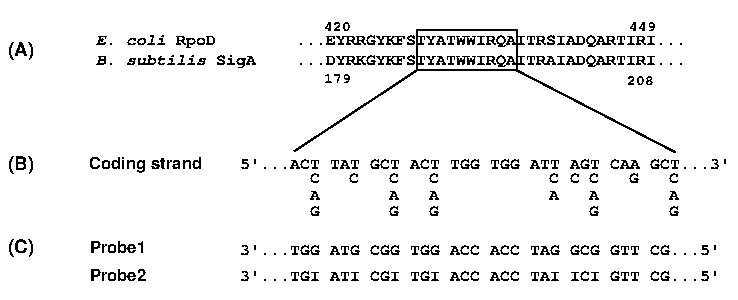
\includegraphics{figures/chap3_rpod_box}
\caption[Design of ``\textit{rpoD} box'' probe]{Design of
``\textit{rpoD} box'' probe. \textbf{(A)} Alignment of the
\textit{E. coli} RpoD and \textit{B. subtilis} SigA. The numbers
above the \textit{E. coli} sequence and the below \textit{B.
subtilis} sequence are the amino acid residues. The boxed amino
acids denote the ``\textit{rpoD} box''. \textbf{(B)} The deduced
coding strand showing the possible nucleotide sequence.
\textbf{(C)} shows the synthesized oligomers. Probe1 is a
"guessmer", synthesized considering the high GC codon bias in
\emph{Pseudomonas}. Note the use of inosine for degenerate
positions in Probe2. Modified and redrawn from
\citet{Tanaka1988}.} \label{chap3:rpod_box}
\end{figure}

Earlier studies in our laboratory had identified and cloned a
genomic fragment from Lz4W using Probe1 in
Figure~\ref{chap3:rpod_box}C. The plasmid was sequenced using
subcloning of the restriction fragments in pUC19. It contained a
\U{5.2}{kb} insert spanning partial \emph{pot} and \emph{pho}
operon with no apparent sequence similarity with any known
$\sigmaup$ gene (data not shown).

In order to circumvent the problem associated with the
non-specificity of the Probe1, the second degenerate probe, Probe2
was synthesized (Figure~\ref{chap3:rpod_box}C). Probe2, when used
in Southern hybridization analysis, detected two bands in genomic
DNA digested with \emph{Pst}I (Lane 1 in
Figure~\ref{chap3:rpod_box_southern}). To clone these two DNA
fragments a  partial genomic library was made by eluting the DNA
from these bands and ligating the eluted DNA to pUC19. Even after
repeated screening, we failed to detect any positive clone in the
library generated from the DNA of the upper band. However, a
positive clone was detected in the library, made using DNA from
the lower band. Upon sequencing the plasmid, it was found that the
\U{2}{kb} insert of the plasmid contains two ORFs very similar in
sequence to that of \emph{trk}, \emph{fmu} sequences of \emph{E.
coli} (data not shown), with no apparent sequence similarity to
any known $\sigmaup$ factor. Nevertheless, another set of
libraries were made in pBluescriptII KS+, using the DNA eluted
from the same positive bands. Once again the probe failed to
detect any positive clone in library made from the DNA of the
upper band. On screening the library made with the DNA eluted from
the lower band, the probe again detected the false positive clone
containing \emph{trk} and \emph{fmu}, for the second time. The
reason why the Probe2 binds to this DNA fragment is still
unexplainable.

\begin{figure}[tbp]
\centering
\includegraphics{figures/chap3_rpod_box_southern}
\caption[Genomic Southern blot analysis using ``\emph{rpoD} box''
probe]{%
    Genomic Southern hybridization analysis using ``\emph{rpoD} box''
    probe. Probe2 in Figure~\ref{chap3:rpod_box}C was used to
    probe genomic DNA of Lz4W digested with several enzymes. The
    positive bands on \emph{Pst}I digested DNA was marked with
    arrows on the left side. Right side shows the calculated
    marker positions. The numbers on the top shows the lane
    numbers. Lane 1, Lz4W genomic DNA digested with \emph{Pst}I;
    lane2, Lz4W genomic DNA digested with \emph{Eco}RI; lane 3,
    Lz4W genomic DNA digested with \emph{Xho}I; lane 4, plasmid
    pGEMD~\citep{Igarashi1991} digested with \emph{Hin}dIII which
    contains the full-length \emph{rpoD} gene of \emph{E. coli},
    loaded as positive control.}
\label{chap3:rpod_box_southern}
\end{figure}

\subsubsection{Full-length genes as heterologous probes}

Having failed to detect any true positive clone with the
``\e{rpoD} box'' oligomeric probe, an alternative strategy was
considered. The suitability of the full length \emph{rpoD} of
\emph{E. coli} and \emph{P. aeruginosa} gene as heterologous
probes was tested in genomic Southern blot analysis. The
\U{2.1}{kb} \emph{Hin}dIII fragment containing the full-length
\emph{rpoD} of \emph{E. coli} from plasmid
pGEMD~\citep{Igarashi1991} and \U{2.3}{kb} \emph{Pst}I insert from
plasmid pASB3~\citep{Tanaka1991} containing the full-length
\emph{rpoD} of \emph{P. aeruginosa} were used. Both these genes,
when used as probes for genomic Southern hybridization analysis,
bound poorly to the Lz4W genomic DNA under high stringency.

\emph{P. aeruginosa rpoS} gene, on the other hand, bound strongly
to Lz4W genomic DNA, as shown in the
Figure~\ref{chap3:pdb18r_southern}. The \U{$\sim$1.8}{kb}
\emph{Kpn}I--\emph{Hin}dIII insert from the plasmid
pDB18R~\citep{Fujita1994}, spanning the full-length \emph{rpoS} of
\emph{P. aeruginosa}, was used as probe in Southern blot analysis.
The position of the positive bands in the lane containing
\emph{Pst}I digested DNA (lane 1 in
Figure~\ref{chap3:pdb18r_southern}B) was identical to what was
observed with ``\emph{rpoD} box'' probe (lane 1 in
Figure~\ref{chap3:rpod_box_southern}). This indicated that the
lower band detected by ``\emph{rpoD} box'' probe in \emph{Pst}I
digested genomic DNA of Lz4W was presumably the \emph{rpoS}
homolog.

\begin{figure}[tbp]
\includegraphics{figures/chap3_pdb18r_southern}
\caption[Genomic Southern blot analysis using \emph{P. aeruginosa
rpoS} as probe]{%
    Genomic Southern hybridization analysis using \emph{P. aeruginosa rpoS}
    as probe. \textbf{(A)} shows the probe used. The \U{$\sim$1.8}{kb} \emph{Kpn}I--\emph{Hin}dIII insert from
    plasmid pDB18R~\citep{Fujita1994} was used to probe the genomic DNA of Lz4W digested with various enzymes.
    The line below the map shows the span of the probe used. \textbf{(B)} shows the autoradiogram. Numbers along the right side
indicate the markers in base-pairs. The positive bands are shown
with arrows on the left. Approximately \mug{3} digested DNA was
loaded in each lane. The enzymes used are indicated on the top of
each lane and numbers below each lane show the lane numbers. Lane
1, \emph{Pst}I; lane 2, \emph{Pst}I and \emph{Bam}HI; lane 3,
\emph{Pst}I and \emph{Eco}RI; lane 4, \emph{Pst}I and \emph{Sal}I;
lane 5, \emph{Pst}I and \emph{Xho}I.}
\label{chap3:pdb18r_southern}
\end{figure}

\subsubsection{Functional complementation of \emph{E. coli rpoS}
mutant}

With the idea that the lower band (\U{$\sim$2}{kb}) detected by
the ``\emph{rpoD} box'' in \emph{Pst}I digested genomic DNA of
Lz4W was probably \emph{rpoS} homolog, an attempt was made to
clone the gene by functional complementation of \emph{E. coli
rpoS} mutant. The strategy was to make use of a strain of \emph{E.
coli} called ZK918~\citep[see Table~\ref{ecolistrains} on page
\pageref{ecolistrains} for genotype]{Bohannon1991}. This strain is
\emph{rpoS}-deficient due to a deletional insertion generated with
a \emph{rpoS}::Km fusion. The strain also carries a chromosomal
insertion of a transcriptional fusion of \emph{bolAp1} promoter to
the \emph{lacZ} at the \emph{bolA} locus. Because
\emph{bolAp}$_{1}$ promoter is \emph{rpoS}-dependent, the
phenotype of the strain was reported to be RpoS\su{$-$}
LacZ\su{$-$}~\citep{Bohannon1991,Ramos1998}. The strain had been
used earlier to clone \emph{rpoS} homolog from \emph{P. putida}
KT2440~\citep{Ramos1998}.

A partial genomic library was made with the DNA eluted from the
lower band (lane 1 in Figure~\ref{chap3:rpod_box_southern}) in
pBluescriptII KS+ vector and electroporated into ZK918. An aliquot
of the cells was plated on kanamycin, ampicillin and X-gal
containing LB agar plates without any treatment. Since \emph{rpoS}
is known to confer acid-resistance, \emph{rpoS} containing cells
were enriched by first treating the cells with acid, and then
neutralizing, before plating on selection plates. For acid
treatment, \mul{200} of transformed cells in LB was treated with
\mul{10} of \U{1}{N} HCl for \U{30}{min}. The suspension was then
neutralized by addition of \mul{10} of \U{1}{N} NaOH before
plating on ampicillin, kanamycin and X-gal containing plates. It
was observed that ZK918 cells had too high background
$\betaup$-galactosidase activity to visually distinguish between
RpoS\su{$-$} and RpoS\su{$+$} cells. An attempt was made to select
the cells with higher $\betaup$-galactosidase activity by plating
the cells in lactose minimal media containing ampicillin and
kanamycin. But even on these plates the \emph{rpoS} harboring
cells were indistinguishable from the background control cells.

\subsubsection{Use of degenerate primers}
Due to the failures in strategies described above, degenerate PCR
primers were designed from the most conserved regions of
$\sigmaup$\su{70} family as shown in Figure~\ref{chap3:primers}.
The forward primers, RPODFP1 and RPODFP2, were designed from
region 2.3/2.4 and reverse primers, RPODRP1 and RPODRP2, were
designed from region 4.2 (Figure~\ref{chap3:primers}C). The
primers were designed with different level of degeneracies. Both
these primers when used in PCR with Lz4W genomic DNA as template,
amplified a \U{400}{bp} DNA fragment. The amplified DNA was
purified from the gel and cloned into TA cloning vector pGEM-T.
Four positive clones carrying insert, were detected, and named as
pT1, pT6, pT7, and pT9. The inserts in these clones were named T1,
T6, T7, and T9 respectively. All these inserts were sequenced and
a careful examination of the sequence and database search using
BLAST revealed that the T1 is a fragment of \emph{rpoS}, and T7 is
a fragment of \emph{rpoD}. T6 and T9 were generated by fusion of
\emph{rpoS} and \emph{rpoD} DNA fragments as PCR artifacts. The
BLAST result of T1 and T7 are summarised in
Table~\ref{chap3:blast_summary}.

\begin{sidewaysfigure}[tbp]
\includegraphics{figures/chap3_1}
\caption[Primer design strategy]{Primer design strategy. (A)
\emph{E.coli} (GenBank accession  J01687), \emph{P. putida}
(GenBank accession D30045) and \emph{P. aeruginosa} (GenBank
accession D90118) \emph{rpoD} sequences were aligned. Only the
regions used to design primers (from 2.3/2.4 and 4.2) are shown.
(B) The corresponding nucleotide sequence alignment is shown with
the bottom most track showing the degeneracy at the third codon
position. (C) and (D) show the pairs of degenerate primers
designed. The degeneracy was reduced considering the high GC
content of \emph{Pseudomonas} sp. genome.} \label{chap3:primers}
\end{sidewaysfigure}

\begin{table}[tbp]
\begin{minipage}[c]{\textwidth}
\renewcommand{\footnoterule}{}
\caption[Summary of BLASTX statistics for PCR amplified
\emph{rpoD} and \emph{rpoS} fragments]{Summary of BLASTX
statistics for PCR amplified \emph{rpoS} and \emph{rpoD}
fragments\protect\footnote{The top five BLASTX hit statistics are
shown for each case}} \label{chap3:blast_summary} \centering
\begin{small}
\begin{tabular}{llccc}\toprule
\textbf{Organism} & \textbf{Gene} & \textbf{Accession} &
\textbf{Score} & \textbf{E-value}\\\midrule\addlinespace
\multicolumn{5}{l}{\textbf{Fragment T1}}\\ \emph{Pseudomonas
tolaasii} & \emph{rpoS} & AB006073 & 114 & $3
\times{}10^{-43}$ \\
\emph{Pseudomonas fluorescens} & \emph{rpoS} & U34203 & 115 &
$4\times{}10^{-43}$ \\
\emph{Pseudomonas syringae} pv. tomato & \emph{rpoS} & AF061853 &
114  & $8\times{}10^{-43}$ \\
\emph{Pseudomonas putida}& \emph{rpoS} & X91654 &
113 & $2\times{}10^{-42}$\\
\emph{Pseudomonas aeruginosa} & \emph{rpoS} & P45684 & 112 &
$3\times{}10^{-41}$\\\addlinespace \multicolumn{5}{l}{\textbf{Fragment T7}}\\
\emph{Pseudomonas fluorescens} & \emph{rpoD} & P52326 & 189 &
$8\times{}10^{-48}$ \\
\emph{Pseudomonas putida} & \emph{rpoD} & U93292 &  189 &
$8\times{}10^{-48}$ \\
\emph{Pseudomonas tolaasii} & \emph{rpoD} &AJ007830 &  189 &
$8\times{}10^{-48}$ \\
\emph{Pseudomonas aeruginosa} & \emph{rpoD} & P26480 &  188 & $2\times{}10^{-47}$ \\
\emph{Pseudomonas putida} & \emph{rpoD} & P52327 &  186 &
$7\times{}10^{-47}$ \\
\bottomrule
\end{tabular}
\end{small}
\end{minipage}
\end{table}

When used as probe in genomic Southern hybridization analysis, all
these DNA fragments hybridized strongly to Lz4W genomic
DNA(Figure~\ref{chap3:tprobes}). Although T6 is a PCR artifact, it
gave expected Southern pattern (lanes 2--6 in
Figure~\ref{chap3:tprobes}). T1 being \emph{rpoS} fragment, bound
to the lower \emph{Pst}I band (lane 1 in
Figure~\ref{chap3:tprobes}) and T7 bound to the upper band (lane 7
in Figure~\ref{chap3:tprobes}). This result also confirmed that
the \U{$\sim$4}{kb} \emph{Pst}I band indeed contained \emph{rpoD},
and the \U{$\sim$2}{kb} \emph{Pst}I band contained \emph{rpoS}.
The result also indicated that there was a \emph{Bam}HI site
within both \emph{rpoD} and \emph{rpoS} (lane 3), and that  a
\emph{Sal}I site exists within \emph{rpoD} (lane 5 in
Figure~\ref{chap3:tprobes}).

\begin{figure}[tbp]
\centering
\includegraphics{figures/chap3_tprobe_southern.pdf}
\caption[Southern blot analysis using PCR-amplified \emph{rpoD}
and \emph{rpoS} fragments]{%
    Southern blot analysis of Lz4W genomic DNA using PCR-amplified \emph{rpoD} and \emph{rpoS}
    fragments. The numbers on the right side indicates the marker
    is base-pairs. The probes used are marked below (for the
    description of the probes, see
    Table~\ref{chap3:blast_summary} and text). The positive bands are indicated by arrows on the left. The enzymes used for digestion of genomic DNA are
    indicated on top. Lane 1, 2 and 7, \emph{Pst}I; lane 3,
    \emph{Pst}I and \emph{Bam}HI; lane 4, \emph{Pst}I and
    \emph{Eco}RI; lane 5, \emph{Pst}I and \emph{Sal}I; lane 6,
    \emph{Pst}I and \emph{Xho}I.}
\label{chap3:tprobes}
\end{figure}

\subsubsection{Complementation of \emph{E. coli rpoD} mutant}

With the indication that the bigger \emph{Pst}I fragment probably
contained \emph{rpoD}, an attempt was made to clone the gene by
functional complementation of \emph{E. coli rpoD} mutant. For
complementation,  a strain of \emph{E. coli} named UQ285 was used,
which harbors a temperature-sensitive \emph{rpoD}
allele~\citep{Isaksson1977}. This strain was unable to grow at
42\dg{} unless complemented by a fully functional \emph{rpoD}\@.
The DNA extracted from the \U{$\sim$4}{kb} region of the gel was
ligated to plasmid pBluescriptII KS+, and electroporated into
UQ285. The transformed cells were plated on LB agar plates
containing ampicillin, and incubated at 42\dg{}. Surprisingly,
there were no complemented clone. This suggested that either the
fragment does not contain the full-length gene of \e{rpoD}, or the
gene was not functional in \bact{Ec}. The inability of Lz4W
\e{rpoD} to complement the functions of \bact{Ec} \e{rpoD} also
could not be ruled out.

To test the idea whether the high-copy number of the vector
pBluescriptII KS+ that was used for complementation was having a
detrimental effect on the cell survival, the complementation
experiment was repeated using a low-copy number vector
pCL1920~\citep{Lerner1990}. Even in this case there was no
complemented clone.

\subsubsection{Cloning of \emph{rpoD} in fragments}

After the failure in cloning the full-length \e{rpoD}, an attempt
was made to clone the gene in separate fragments, taking advantage
of the presence of a single \emph{Sal}I site within the gene.
Following separation of the \emph{Pst}I and \emph{Sal}I digested
genomic DNA on preparative agarose gel, DNA from the \U{2}{kb}
region was extracted and a partial genomic library was made in
pBluescriptII KS+. A positive clone was detected using the T7
probe. The plasmid isolated from this clone, p4A4, was almost
fully sequenced. Database search revealed that it contained a
partial ORF at the \emph{Sal}I end and another partial ORF at the
\emph{Pst}I end. Upon running BLAST against GenBank we found that
the clone contained partial ORF of \emph{rpoD} at the \emph{Sal}I
end. A map of the insert is shown in Figure~\ref{chap3:4a4}A and
the sequence of the partial \emph{rpoD} is shown in
Figure~\ref{chap3:4a4}B. The summary of the BLAST statistics is
shown in Table~\ref{chap3:4a4_blast}. The highest similarity of
the aligned region was with \emph{P. tolaasii} (BLAST positive,
98\%) and with \emph{P. fluorescens} (BLAST positive 98\%).
According to the alignment, the cloned \emph{rpoD}$_{Lz4W}$
started from the codon 314 of \emph{P. tolaasii} \emph{rpoD} and
codon 315 of \emph{P. fluorescens}. The \emph{E. coli rpoD} was
only 89\% (BLAST positives) similar. All similarity scores were
calculated using BLOSUM62 matrix.

\begin{sidewaysfigure}[tbp]
\centering
\includegraphics{figures/chap3_4a4}
\caption[\emph{rpoD} homolog of Lz4W]{\textbf{(A)}Schematic
diagram of the insert in p4A4, drawn to  scale. Broken arrows
denote partial ORFs. Dotted line indicates the region not
sequenced. \textbf{(B)} The sequence of the partial \emph{rpoD}
homolog of Lz4W. Translated amino acids are shown below the
sequence. The underlined sequence is $\rhoup$-independent
transcription termination signal. \textbf{(C)} The conserved ORF
downstream of \emph{rpoD}. \textbf{(D)} The $\rhoup$-independent
transcription termination signal downstream of \emph{rpoD} ORF
($\Delta$G $-$24.3 kcal/mol).} \label{chap3:4a4}
\end{sidewaysfigure}

\begin{table}[tbp]
\begin{minipage}[c]{\textwidth}

\renewcommand{\footnoterule}{}
\caption[Summary of BLASTX statistics of
\emph{rpoD}$_{Lz4W}$]{Summary of BLASTX statistics of
\emph{rpoD}$_{Lz4W}$\protect\footnote{The top five BLASTX hit
statistics are shown.}} \label{chap3:4a4_blast}
\begin{narrow}{-1in}{-1in} \centering
\begin{small}
\begin{tabular}{llcccc}\toprule
\textbf{Organism} & \textbf{Gene} &
\multicolumn{1}{p{1.1in}}{\textbf{GenBank or Swiss\-Prot
Accession}\protect\footnote{GenBank accession are prepended with
gb: and SwissProt accession are prepended with sp:.}} &
\textbf{Score} & \textbf{E-value} & \textbf{\%
similarity}\protect\footnote{According to BLOSUM62
matrix.}\\\midrule\addlinespace \emph{Pseudomonas tolaasii} &
\emph{rpoD} & gb:AJ007830
 & 583 & $10^{-165}$ & 98 \\
\emph{Pseudomonas fluorescens} & \emph{rpoD} & sp:P52326
 & 583 &$10^{-43}$ &98\\
\emph{Pseudomonas putida} & \emph{rpoD} & sp:P52327 &
539  & $10^{-152}$ & 93\\
\emph{Pseudomonas aeruginosa} & \emph{rpoD} & sp:P26480 & 538 &
$10^{-152}$ & 94\\
\emph{Shewanella violacea} & \emph{rpoD} & sp:O24744 & 507 &
$10^{-143}$ & 91 \\
%\emph{Salmonella typhimurium} & \emph{rpoD} & sp:P07336 &  499 & $10^{-140}$ & 90 \\
\bottomrule
\end{tabular}
\end{small}
\end{narrow}
\end{minipage}
\end{table}

A putative $\rhoup$-independent transcription termination signal
was also detected (Figure~\ref{chap3:4a4}D) downstream of the
\emph{rpoD} ORF. There was also an ORF with domain structure of a
transcription factor as shown in Figure~\ref{chap3:4a4}C. This ORF
is conserved in large group of proteobacteria including \emph{P.
putida}~(GenBank accession AF302763).

\subsubsection{Cloning of \emph{rpoS}}




For cloning of \e{rpoS}, two types of genomic libraries were used,
a cosmid library and a partial genomic library in plasmid. The
cosmid  genomic library was constructed in cosmid
pLAFR3~\citep{Staskawicz1987} as described in
Section~\ref{chap2:cosmid_library}. A simultaneous screening of
the cosmid library and a partial genomic library in plasmid
pBluescriptII KS+ from the \emph{rpoS} region of \emph{Pst}I
digested genomic DNA, was carried out. A positive clone was
detected in the plasmid library using T1 and the insert from
plasmid pDB18R as probes. The plasmid, named p4C12, contained a
\U{$\sim$2}{kb} \emph{Pst}I insert. By subcloning and direct
sequencing with primers full sequence of the insert was
determined. Upon database search it was found that it contained
the full ORF of \emph{rpoS} and a partial ORF from the upstream
\emph{nlpD} gene. The summary of the BLASTX statistics for
\emph{rpoS}$_{Lz4W}$ is shown in Table~\ref{chap3:4c12_blast}. As
shown in the Table~\ref{chap3:4c12_blast} the closest sequence
similarity was with \emph{P. fluorescens} (BLAST positive score,
80\%). The BLAST positive score was only 75\% with \bact{Ec}
\emph{rpoS}. A schematic diagram of the insert in p4C12 is shown
in Figure~\ref{chap3:4c12_map} and the full sequence is shown is
Figure~\ref{chap3:4c12}.


\begin{table}[tbp]
\begin{minipage}[c]{\textwidth}

\renewcommand{\footnoterule}{}
\caption[Summary of BLASTX statistics of
\emph{rpoS}$_{Lz4W}$]{Summary of BLASTX statistics of
\emph{rpoS}$_{Lz4W}$\protect\footnote{The top five BLASTX hit
statistics are shown.}} \label{chap3:4c12_blast}
\begin{narrow}{-1in}{-1in}
\centering
\begin{small}
\begin{tabular}{@{}llcccc@{}}\toprule
\textbf{Organism} & \textbf{Gene} &
\multicolumn{1}{p{0.7in}}{\textbf{GenBank accession}} &
\textbf{Score} & \textbf{E-value} & \textbf{\%
similarity}\protect\footnote{According to BLOSUM62
matrix.}\\\midrule\addlinespace \emph{Pseudomonas fluorescens} &
\emph{rpoS} & gb:AAB02846
 & 490 & $10^{-137}$ & 80 \\
\emph{Pseudomonas putida} & \emph{rpoS} & gb:CAB46191
 & 483 &$10^{-135}$ & 80\\
\emph{Pseudomonas syringae} pv. tomato & \emph{rpoS} & gb:AAC16326 & 482  & $10^{-135}$ & 79\\
\emph{Pseudomonas syringae} pv. syringae & \emph{rpoS} &
gb:AAF20993 & 481 &
$10^{-134}$ & 79\\
\emph{Pseudomonas tolaasii} & \emph{rpoS} & gb:BAA21674 & 480 & $10^{-134}$ & 78 \\
%\emph{Salmonella typhimurium} & \emph{rpoD} & sp:P07336 &  499 & $10^{-140}$ & 90 \\
\bottomrule
\end{tabular}
\end{small}
\end{narrow}
\end{minipage}
\end{table}

Interestingly, the reading frame of \emph{rpoS} was interrupted
with an amber at position 253. The position of this amber is shown
in Figure~\ref{chap3:4c12_map} with an arrow. A putative ribosome
binding site upstream of \emph{rpoS} and a putative
$\rhoup$-independent transcription termination site downstream of
\emph{rpoS} were readily identified (Figure~\ref{chap3:4c12}).

\begin{figure}[tbp]
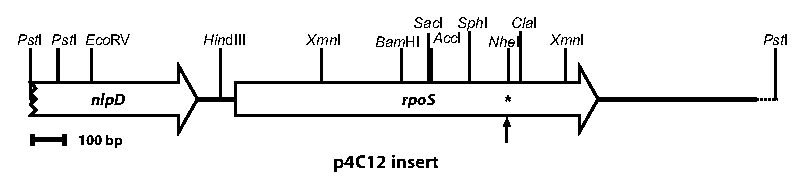
\includegraphics{figures/chap3_4c12_map}
\caption[Schematic map of plasmid p4C12]{Schematic map of plasmid
p4C12 drawn to  scale. The arrows indicate reading frames. The
broken arrow indicates partial reading frame. The dotted portion
at the end indicates the region not sequenced. Note the position
of the \emph{Nhe}I site created by a G to T transversion at
position 1324 of the sequence. The mutation results E253 to change
to an \emph{amber}. The position of the \emph{amber} is shown by
``$\ast$'' and marked with a arrow.} \label{chap3:4c12_map}
\end{figure}



\subsection{\emph{rpoS} homolog of Lz4W contains an amber}




The occurrence of the amber mutation within the reading frame of
\lzsig{} raised the possibility that the mutation might have
occurred during propagation of the plasmid p4C12 in \bact{Ec}. To
rule out this possibility, plasmids from several clones were
sequenced. It was confirmed that all the clones contain the amber
within the \e{rpoS} reading frame. The corresponding region of the
electrophoretogram is shown in Figure~\ref{chromatogram}.
Interestingly, the presence of the amber caused the creation of a
unique \emph{Nhe}I site. Taking advantage of this fact we tested
whether the amber is present in genomic sequence of Lz4W.

\begin{figure}[tbp]
\centering
\includegraphics{figures/chap3_4c12}
\caption[\emph{rpoS} homolog of Lz4W]{The complete sequence of the
insert in plasmid p4C12 except a few terminal nucleotides. The
partial reading frame of \emph{nlpD} and the full sequence of
\emph{rpoS} with translated amino acids are shown. The reading
frames are indicated in lower case. Shine-Dalgarno sequence
(labelled SD), "\emph{rpoD} box", and $\rhoup$-independent
terminator sequence, with convergent arrows denoting the
complementary region of the hairpin loop, are indicated. Note the
presence of an amber codon in position 1324 of the sequence
(marked with $\ast$) and the resulting creation of \emph{Nhe}I
site within \emph{rpoS} reading frame. The amino acids are shown
in single letter code.} \label{chap3:4c12}
\end{figure}

The presence of the amber within \emph{rpoS} reading frame was
tested in two independent lines of Lz4W that were maintained in
our laboratory in parallel. Presence of \emph{Nhe}I site within
the reading frame would indicate the presence of amber. If
present, the \emph{Nhe}I site, upon digestion would split the
\U{$\sim$2.1}{kb} \emph{Pst}I fragment into 2 fragments with sizes
1300 and \U{740}{bp}. Lz4W genomic DNA, isolated from both the
lines of Lz4W was digested with \emph{Pst}I, and \emph{Pst}I plus
\emph{Nhe}I, and was probed with the insert from p4C12
(Figure~\ref{chap3:amber}).

\begin{figure}[tbp]
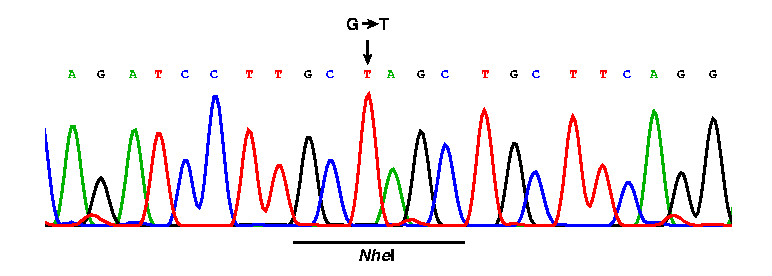
\includegraphics{figures/chap3_chromatogram.pdf}
\caption[Chromatogram of \emph{rpoS} showing the
\emph{amber}]{Portion of the chromatogram of p4C12 showing the
amber. The G to T transversion at position 1324 is marked. The
\emph{Nhe}I site created due to \emph{amber} is also shown.}
\label{chromatogram}
\end{figure}

As shown in Figure~\ref{chap3:amber} both the lines of Lz4W had
the internal \e{Nhe}I site. In \emph{Pst}I and \emph{Nhe}I double
digested DNA the \emph{rpoS} band was split into two fragments of
1300 and \U{750}{bp} in size (lanes 2 and 4 in
Figure~\ref{chap3:amber}). The residual \emph{rpoS} bands in both
these lanes was because of incomplete digestion by \emph{Nhe}I.
\begin{figure}[tbp]
\centering
\includegraphics{figures/chap3_amber}
\caption[Presence of amber with \emph{rpoS} reading
frame]{Presence of amber within \emph{rpoS} reading frame in Lz4W
genome. Genomic DNA isolated from two independently maintained
lines of Lz4W was probed with p4C12 insert in Southern
hybridization. \emph{rpoS} band and two smaller fragments created
by \emph{Pst}I and \emph{Nhe}I double digestion is marked with
arrows. The enzymes used are indicated on top and the lane numbers
are indicated below. Lane 1, Lz4W line 1 digested with
\emph{Pst}I; lane 2, Lz4W line 1 digested with both \emph{Pst}I
and \emph{Nhe}I; lane 3, Lz4W line 2 digested with \emph{Pst}I;
lane 4, Lz4W line 2 digested with both \emph{Pst}I and
\emph{Nhe}I.} \label{chap3:amber}
\end{figure}
\subsection{Southern analysis using \emph{P. aeruginosa rpoH} as
probe}

To explore the suitability of using \emph{P. aeruginosa rpoH} gene
coding for the heat-shock $\sigmaup$ factor, $\sigmaup$\su{32}, as
heterologous probe for cloning the corresponding gene from Lz4W,
the gene was used in Southern hybridization analysis. A
\U{1.9}{kb} \emph{Sal}I--\emph{Pst}I fragment from plasmid
pRPOH5~\citep{Aramaki1996}, spanning the full-length \emph{rpoH}
of \bact{Pa} was used as heterologous probe in Southern analysis
of Lz4W genomic DNA, digested with several enzymes
(Figure~\ref{chap3:rpoh_southern}). As shown in the figure, a
\emph{Sal}I fragment of around \U{3}{kb} strongly binds to the
probe, suggesting its presence and similarity with the Lz4W gene.
The binding also suggested the feasibility of using this gene as
probe for cloning the homolog from Lz4W.

\begin{figure}[tbp]
\centering
\begin{narrow}{-1in}{0in}
\flushright
\includegraphics{figures/chap3_rpoh}
\end{narrow}
\caption[Southern analysis using \emph{P. aeruginosa rpoH}]{%
    Southern hybridization analysis using \emph{P. aeruginosa rpoH} as probe. \textbf{(A)} Schematic diagram of the probe
    used. A \U{1.9}{kb} \emph{Sal}I--\emph{Pst}I fragment from
    plasmid pRPOH5~\citep{Aramaki1996} spanning the full-length \emph{rpoH}
    of \emph{P. aeruginosa} was used to probe the genomic DNA
    of Lz4W, digested with various enzyme. The solid line below
    the map indicates the span of the probe. \textbf{(B)}
    shows the autoradiogram. Numbers along the right side
    indicate the markers in base-pairs. Approximately \mug{3} digested
    DNA was loaded in each lane. The enzymes used are indicated on the
    top of each lane and numbers below each lane show the lane
    numbers. Lane 1, \emph{Xba}I; lane 2, \emph{Sal}I; lane 3, \emph{Hin}dIII;
    lane 4, \emph{Bam}HI.}
\label{chap3:rpoh_southern}
\end{figure}



\subsection{Southern analysis using \bact{Ec} \emph{rpoA} as probe}

With similar intention to that of \e{rpoH}, \emph{E. coli}
$\alphaup$ was used as probe in Southern analysis of Lz4W genomic
DNA (\ref{chap3_fig:alpha_southern}), to examine the possibility
of using this gene to clone the homolog from Lz4W. Lz4W genomic
DNA was digested with various restriction enzymes and probed with
an \U{1.2}{kb} \emph{Xba}I fragment from the plasmid pGEMAX185
\citep{Igarashi1991}. As shown in the Figure
\ref{chap3_fig:alpha_southern}, \emph{E. coli rpoA} binds to Lz4W
genomic DNA strongly, suggesting strong sequence homology. A
\emph{Bam}HI fragment of \U{$\sim$7}{kb}, and two \emph{Sal}I
fragments, of sizes \U{$\sim$7}{kb}, and \U{$\sim$4}{kb} were
detected.

\begin{figure}[tbp]

\centering

\includegraphics{figures/chap3_alpha_southern}

\caption[Southern analysis using \emph{E.coli rpoA}
probe]{Southern hybridization analysis using \emph{E. coli rpoA}
probe. \textbf{(A)} Schematic diagram of the probe used. A
\U{1.2}{kb} \emph{Xba}I fragment form plasmid pGEMAX185
\citep{Igarashi1991} was used to probe the genomic DNA from Lz4W
digested with various enzymes. The line below the map shows the
span of the probe used. \textbf{(B)} shows the autoradiogram.
Numbers along the right side indicate the markers in base-pairs.
Approximately \mug{3} digested DNA was loaded in each lane. The
enzymes used are indicated on the top of each lane and numbers
below each lane show the lane numbers. Lane 1, \emph{Xba}I; lane
2, \emph{Sal}I; lane 3, \emph{Hin}dIII; lane 4, \emph{Bam}HI.}

\label{chap3_fig:alpha_southern}

\end{figure}


\subsection{Southern analysis using \emph{rpoB} and \emph{rpoC}}

To examine whether or not \emph{E. coli} \emph{rpoB} and
\emph{rpoC} (coding for $\betaup$ and $\betaup'$ subunits
respectively, of RNA polymerase) hybridize to Lz4W genomic DNA,
genomic Southern analysis was performed using \emph{E. coli}
\emph{rpoB} and \emph{rpoC} genes
(Figure~\ref{chap3:beta_southern}). The \U{10.2}{kb}
\emph{Hin}dIII insert from the plasmid pGEMBC~\citep{Igarashi1991}
containing the full-length \emph{rpoB}, and \emph{rpoC} from
\emph{E. coli} was used as a heterologous probe in genomic
Southern hybridization. We detected very strong hybridization
signals, indicating very strong sequence conservation between
these genes.

\begin{figure}[tbp]

\centering

\includegraphics{figures/chap3_beta_southern}

\caption[Southern analysis using \emph{E. coli rpoB} and
\emph{rpoC}]{Southern hybridization analysis of Lz4W genomic DNA
using \emph{E. coli rpoB} and \emph{rpoC} as probe. The
\U{10.2}{kb} \emph{Hin}dIII insert from plasmid pGEMBC
\citep{Igarashi1991} was used to probe Lz4W genomic DNA digested
with various restriction enzymes. \textbf{(A)} Schematic diagram
of the probe used. The insert contained the full-length
\emph{rpoB} and \emph{rpoC} gene of \emph{E. coli} with upstream
\emph{rplL}. The solid line below the map shows the span of the
probe used. \textbf{(B)} The autoradiogram. Approximately
\mug{3--4} of digested genomic DNA was used in each lane. The
enzymes are indicated on top. The numbers along the right hand
side indicate the marker positions in base-pairs. The numbers
below mark the lanes. Lane 1, \emph{Xba}I; lane 2, \emph{Sal}I;
lane 3, \emph{Hin}dIII and lane 4, \emph{Bam}HI.}

\label{chap3:beta_southern}

\end{figure}


\section{Discussion}

$\sigmaup$ factors of proteobacteria are conserved in their
sequences, structures and functions in evolution. Several
$\sigmaup$ factors were cloned exploiting the close sequence
similarities. Traditionally, an oligomer, named ``\emph{rpoD}
box'', designed from the most conserved regions 2.3/2.4 had been
used to clone various members of $\sigmaup$\su{70} family of
$\sigmaup$ factors. Although, $\sigmaup$ factors from
Gram-positive bacteria and Gram-negative bacteria differ in their
molecular weight and overall amino acid sequence (\emph{e.g.},
\emph{B. subtilis} primary $\sigmaup$ factor is of the size
\U{43}{kDa} and \emph{E. coli} vegetative $\sigmaup$ is of the
size \U{70}{kDa}), distinct sequence similarities in several
domains enabled the cloning of $\sigmaup$ factors by heterologous
probes. Not only the primary $\sigmaup$ factors, but other members
of $\sigmaup$\su{70} family of \emph{E. coli} (\emph{rpoH},
\emph{rpoS}) are interchangeable in function across species,
enabling functional complementation by these genes.

In this study, \emph{rpoD} and \emph{rpoS} gene fragments were
amplified using degenerate PCR primers, designed from the most
conserved region of the $\sigmaup$\su{70} family. Using the
amplified fragment a partial ORF coding for \emph{rpoD} was
cloned. A full-length ORF coding for \emph{rpoS} of Lz4W was also
cloned using the amplified fragment and \bact{Pa} \emph{rpoS} gene
as probes. Both \emph{rpoD} and \emph{rpoS} homologs show strong
sequence similarities with the corresponding genes of other
pseudomonads. Interestingly, the \emph{rpoS} gene of Lz4W is
interrupted at codon 253 by an amber. The implications of this
mutation in this organism was investigated further, the results of
which are presented in subsequent chapters.

Several standards method of cloning \siga{} family members were
not successful. The attempt to clone $\sigmaup$ gene using
``\emph{rpoD} box" probe failed, in spite of it providing strong
signals in Southern hybridization. Two false positives were
detected using this probe. One of them contained \emph{trk} and
\emph{fmu} homologs of \emph{E. coli}. This clone was detected in
two independent partial genomic libraries of Lz4W. As there is no
evidence of any sequence similarity between this clone and
``\emph{rpoD} box'', there is no explanation for the reason of
strong signals detected using the oligomer. The other false
positive contained partial \emph{phoB} and \emph{pot} operon. In
this case there is prior evidence of false binding of \emph{E.
coli rpoS} probe to \emph{Bradyrhizobium japonicum
phoB}~\citep{Minder1998}.

The cloning attempt by complementation of \bact{Ec} \e{rpoD}
mutant UQ285 was not successful. Among several possible
explanations mentioned earlier, the possibility of a toxic effect
of Lz4W \e{rpoD}, when cloned in \bact{Ec} merits attention. As
shown, the gene, when fragmented, could be readily cloned in
\emph{E. coli}, implicating a toxic effect of the full-length
gene. The cloned part of \emph{rpoD} shows strong sequence
conservation with \emph{rpoD} of other pseudomonads.

Inability of Lz4W \emph{rpoS} to complement \bact{Ec} \e{rpoS}
mutant ZK918 could be easily explained because of the presence of
amber within the \emph{rpoS} reading frame of Lz4W. In later
Chapters we provide evidence that this \emph{rpoS} allele is
unable to induce \emph{bolAp1} promoter to such as extent, so as
to be able to distinguish cells harboring \emph{rpoS} from the
background.

Additionally, Lz4W $\alphaup$, $\betaup$, $\betaup'$, and
$\sigmaup$\su{H}, coded by \emph{rpoA}, \emph{rpoB}, \emph{rpoC}
and \emph{rpoH} respectively, are  similar to the respective
homologs in other bacteria, at the primary sequence level. This
conclusion is based on the strong signals detected in Southern
hybridization analysis of Lz4W genomic DNA with heterologous
probes, enabling the future cloning of these subunits by
heterologous probes, a possibility.\ding{45}


\FloatBarrier\pagebreak \thispagestyle{empty}
\begin{figure}[h]
\raggedleft
\includegraphics{figures/chap4_sep}
\end{figure}
\thispagestyle{empty}

\mathversion{bold}
\chapter{Sequence Analysis of \s{} factors}
\mathversion{normal}

\section{Introduction}

There are a plethora of \s{} factor sequences submitted to
databases in recent years. Yet, a detailed analysis of primary
sequences of the \s{} factors, particularly, comparative genomics
data elucidating the evolution of \s{} factors is yet to come.
This Chapter is the results of one such attempt.

In this Chapter the results of a detailed sequence comparison of
the primary \s{} factors from the viewpoint of cold-adaptation,
followed by the sequence comparison of \e{rpoS} is discussed. The
discussion on \e{rpoS} is primarily focused on  information that
could be derived from the sequence comparison on the regulation of
\e{rpoS} in Lz4W.

\section{Results}

\mathversion{bold}
\subsection{Sequence comparison of primary \s{} factors}
\mathversion{normal}

Sequences of the primary \s{} factors  were collected from
SwissProt database. There were 44 unique full-length sequences
present in this database. All these sequences with their length
and predicted molecular weight are listed in
Table~\ref{rpod_table}. The collection contained two known
cold-adapted bacteria, the deep-sea barophilic \e{Shewanella
violacea} and psychrotroph \e{Listeria monocytogenes}. A multiple
alignment of these sequences with two sequences of \e{Thermus
aquaticus} and \e{Thermus thermophilus} and Lz4W RpoD (\Lzsiga{})
is shown in Figure~\ref{rpod_align}. It was evident from the
alignment that the cloned fragment of \lzsiga{} contained a part
of non-conserved region between regions 1.2 to 2. The cloned
region also contained the rest of the C-terminal end of the RpoD.
A comparison the sequences with important functions is discussed
below. For all discussion in this Chapter, sequence number will be
referred in terms of \bact{Ec} RpoD.

\begin{table}
\begin{minipage}[c]{\textwidth}
\linespread{1}\normalsize \renewcommand{\arraystretch}{1.3}
\renewcommand{\footnoterule}{}
\caption[Primary \s{} factors in SwissProt database]{Primary \s{}
factors in SwissProt database. Only full-length sequences were
considered. Two sequences of \e{Thermus aquaticus} and \e{Thermus
thermophilus} were collected from GeneBank and the accession
numbers are shown with prefix ``gb:''.} \label{rpod_table}
\begin{narrow}{-1in}{-1in}
\centering
\begin{small}
\begin{tabular}{@{}llllp{.7in}@{}}\toprule
\textbf{Species} & \textbf{Key} & \textbf{Accession} &
\textbf{Length (aa)} & \textbf{Molecular Weight (Da)}\\\midrule
{\it Agrobacterium tumefaciens} & Atumefaciens &     P33452 &        684 &      77399 \\

{\it Anabaena} sp.  &   Anabaena &     P26683 &        390 &      45641 \\

{\it Bacillus halodurans} & Bhalodurans &     O66381 &        372 &      42740 \\

{\it Bacillus subtilis} &  Bsubtilis &     P06224 &        371 &      42957 \\

{\it Borrelia burgdorferi } & Bburgdorferi &     P52323 &        631 &      73642 \\

{\it Buchnera aphidicola } & Baphidicola &     P32001 &        617 &      71469 \\

{\it Caulobacter crescentus} & Ccrescentus &     P52324 &        652 &      72675 \\

{\it Chlamydia muridarum} & Cmuridarum &     P56835 &        571 &      66196 \\

{\it Chlamydia pneumoniae } & Cpneumoniae &     Q9Z7F0 &        572 &      66305 \\

{\it Chlamydia trachomatis} & Ctrachomatis &     P18333 &        571 &      66133 \\

{\it Clostridium acetobutylicum} & Cacetobutylicum &     P33656 &        378 &      43260 \\

{\it Enterococcus faecalis} &  Efaecalis &     P52329 &        368 &      41845 \\

{\it Escherichia coli} &      Ecoli &     P00579 &        613 &      70263 \\

{\it Haemophilus influenzae} & Hinfluenzae &     P43766 &        629 &      72084 \\

{\it Helicobacter pylori} &    Hpylori &     P55993 &        671 &      77737 \\

{\it Helicobacter pylori} J99  & HpyloriJ99 &     Q9ZMY3 &        681 &      78763 \\

{\it Lactococcus lactis} (subsp. \e{cremoris}) & Llactiscremoris &     P58290 &        364 &      41579 \\

{\it Lactococcus lactis} (subsp. \e{lactis})  & Llactislactis &     P52330 &        386 &      44079 \\

{\it Leptospira interrogans} & Linterrogans &     P52328 &        377 &      43456 \\

{\it Listeria innocua} &   Linnocua &     Q92BQ6 &        374 &      42446 \\

{\it Listeria monocytogenes} & Lmonocytogenes &     P52331 &        374 &      42419 \\

{\it Microcystis aeruginosa} & Maeruginosa &     P52322 &        416 &      48871 \\

{\it Mycobacterium bovis} &     Mbovis &     Q60162 &        528 &      57800 \\

{\it Mycoplasma genitalium} & Mgenitalium &     P47491 &        497 &      57661 \\

{\it Mycoplasma pneumoniae} & Mpneumoniae &     P78022 &        499 &      57796 \\

{\it Myxococcus xanthus} &   Mxanthus &     P17531 &        708 &      80398 \\

{\it Neisseria gonorrhoeae} & Ngonorrhoeae &     P52325 &        642 &      73679 \\

{\it Pseudomonas aeruginosa} & Paeruginosa &     P26480 &        617 &      69643 \\

{\it Pseudomonas fluorescens} & Pfluorescens &     P52326 &        615 &      69436 \\

{\it Pseudomonas putida} &    Pputida &     P52327 &        614 &      69725 \\

{\it Rhizobium meliloti}  &  Rmeliloti &     Q59753 &        684 &      77173 \\

{\it Rhodobacter capsulatus} & Rcapsulataus &     P46400 &        674 &      75958 \\

{\it Rickettsia prowazekii} & Rprowazekii &     P33451 & 635 &
73080 \\\bottomrule


%\end{minipage}
\end{tabular}
\end{small}
\end{narrow}
\end{minipage}
\linespread{1.1}\normalsize
\end{table}
\begin{table}

\begin{minipage}[c]{\textwidth}
\linespread{1}\normalsize
\renewcommand{\arraystretch}{1.3}
\renewcommand{\footnoterule}{}
\centering {\sffamily\footnotesize\textbf{TABLE~\ref{rpod_table}}\
\ \ \e{Continued.}}\vspace{1em}
\begin{narrow}{-1in}{-1in}
\centering
\begin{small}
\begin{tabular}{@{}llllp{.7in}@{}}\toprule
\textbf{Species} & \textbf{Key} & \textbf{Accession} &
\textbf{Length (aa)} & \textbf{Molecular Weight (Da)}\\\midrule
{\it Salmonella typhimurium} & Styphimurium &     P07336 &        615 &      70530 \\

{\it Shewanella violacea} &  Sviolacea &     O24744 &        614 &      70030 \\

{\it Staphylococcus aureus} &    Saureus &     P26766 &        368 &      42170 \\

{\it Staphylococcus aureus (N315)} & SaureusN315 &     Q99TT5 &        368 &      42156 \\

{\it Streptococcus mutans} &    Smutans &     O33662 &        371 &      42547 \\

{\it Streptococcus pneumoniae} & Spneumoniae &     O08388 &        369 &      42030 \\

{\it Streptomyces aureofaciens} & Saureofaciens &     P27785 &        317 &      35616 \\

{\it Synechococcus} sp. (PCC 7942) & Synechococcus &     P38023 &        384 &      44123 \\

{\it Thermotoga maritima} &  Tmaritima &     P77994 &        399 &      46534 \\

{\it Thermus aquaticus} & Taquaticus & gb:AAG36964 &        438 &      49846 \\

{\it Thermus thermophilus} & Tthermophilus & gb:BAA74758 &        423 &      48494 \\

{\it Treponema pallidum} &  Tpallidum &     O83506 &        611 &      70902 \\

{\it Xylella fastidiosa} & Xfastidiosa &     Q9PDM9 &        618 &
69907 \\\bottomrule
\end{tabular}
\end{small}
\end{narrow}
\end{minipage}
\linespread{1.1}\normalsize
\end{table}
\FloatBarrier


\subsubsection{Core-binding region of RpoD}

As discussed in the Section~\ref{chap1:core_binding}, region 2.2
of \s{} factor, makes extensive contact with the $\betaup'$
subunit. Comparison of these regions showed that, the first three
residues are part of coil and rest is an $\alphaup$ helix. All the
amino acids in this region of \lzsiga{} are identical with the
corresponding residues of other pseudomonads and \bact{Ec}
(Figure~\ref{rpod_align}).

\subsubsection{$-$10 binding and promoter melting}

In Section~\ref{chap1:melting}, it was discussed that the basic
and the aromatic residues in the region 2.3 help in the nucleation
of the strand separation during open complex formation. Comparison
of this region between the cold-adapted species and the
thermophiles revealed that in \e{Thermus} species absolutely
conserved G426 has been replaced by a R residue. All the
differences other than this residues were conserved replacement.
In fact the $\alphaup$ helical portion of this region is
absolutely conserved in all species, particularly, Y430, W433, and
K418 (cyan $\ast$ in Figure~\ref{rpod_align}), which have been
implicated in stacking A($-$11) of the promoter and stabilizing
the separated strands. K414, which is also believed to stabilize
the separated strands, on the other hand is sometimes replaced by
R in many species.

\begin{sidewaysfigure}[tbp]
\centering
\includegraphics{figures/chap4_rpod_align_1}
\caption[Multiple sequence alignment of primary \s{}
factors]{Multiple sequence alignment of primary \s{} factors. All
full-length primary \s{} factors from SwissProt database (see
Table~\ref{rpod_table} for the accession numbers and the name
keys) were aligned using CLUSTALW~\citep{Higgins1996}. The colored
bars on the topmost position showed regions of \s{}, colored as in
Figure~\ref{chap1:sigma}. The tan bars and lines on top indicate
$\alphaup$ helices and coils as in \bact{Ec} \s\smallsu{70}
fragment crystal structure~\citep[][PDB coordinate
1SIG]{Malhotra1996}. The blue bars, the lines, and the dotted
lines below represent the $\alphaup$ helices, coils, and
disordered region observed in \e{T. thermophilus} \s\smallsu{A}
crystal structure~\citep[][PDB coordinate 1IW7]{Vassy2002}. The
ruler numbering indicates \bact{Ec} residue number. The numbering
for Lz4W RpoD corresponds to the internal residue position, for
which the sequence information obtained in the present study. The
N-terminal sequence information is lacking. Important residues are
marked with ``$\ast$'' and colored according to function; promoter
melting, cyan; $-$10 recognition, red; extended $-$10 recognition,
green; $-$35 recognition, blue.} \label{rpod_align}
\end{sidewaysfigure}
\begin{sidewaysfigure}[tbp]
\centering
\includegraphics{figures/chap4_rpod_align_2}
{\footnotesize\bfseries\sffamily
FIGURE~\ref{rpod_align}}~{\footnotesize\sffamily\itshape\
Continued.}
\end{sidewaysfigure}
\begin{sidewaysfigure}[tbp]
\centering
\includegraphics{figures/chap4_rpod_align_3}
{\footnotesize\bfseries\sffamily
FIGURE~\ref{rpod_align}}~{\footnotesize\sffamily\itshape\
Continued.}
\end{sidewaysfigure}

Q437 and T440, which have been shown to contact T($-$12) and R441,
which has been shown to contact $-$13 nucleotide of the promoter
are part of the same $\alphaup$ helix and are also either
conserved, or replaced by similar amino acids in all species (red
$\ast$ in Figure~\ref{rpod_align}).

H455 and E458 have been shown to contact extended $-$10 of the
promoter. Among these H455 is absolutely conserved, whereas E458
has been replaced by a conservative charged residue D in
\e{Helicobacter} (green $\ast$ in Figure~\ref{rpod_align}).

\subsubsection{$-$35 contact sites}

R584, E585 and Q589 of the region 4.2 are the major contact point
of $-$35 site of the promoters. These residues are absolutely
conserved in all bacterial species (blue $\ast$ in
Figure~\ref{rpod_align}).


\subsection{RpoS sequence comparison}

Till date there are 27 unique sequences (full-length) available
for \sigs{} in SwissProt/TrEMBL database. All these sequences with
their predicted molecular weights and lengths are listed in
Table~\ref{chap4:rpos_table}. Except three species from $\betaup$
Proteobacteria and \e{Aquifex}, all other sequences are from
$\gammaup$ Proteobacteria. A multiple alignment of these sequences
with the Lz4W sequence is shown in Figure~\ref{rpos_align}. As
evident from the alignment the reported \e{rpoS}-like sequences
from $\betaup$ Proteobacteria and \e{Aquifex} are quite different
from RpoS sequences from $\gammaup$ Proteobacteria.

\begin{table}
\begin{minipage}[c]{\textwidth}
\renewcommand{\footnoterule}{}
\caption[Known \emph{rpoS} sequences]{\emph{rpoS} sequences in
SwissProt and TrEMBL databases till September,
2002\protect\footnote{Only full-length sequences are shown.
Truncated or incomplete sequences are not considered.}.}
\label{chap4:rpos_table}
\begin{narrow}{-1in}{-1in}
\centering
\begin{small}
\begin{tabular}{@{}llp{.8in}p{.8in}p{.7in}@{}}\toprule
\textbf{Species} & \textbf{Key} & \textbf{Swiss\-Prot/\-Tr\-EMBLE
accession} & \textbf{Length (amino acids)} & \textbf{Molecular
Weight (Da)}\\\midrule\addlinespace
{\it Aquifex aeolicus} & Aaeolicus & O67437 & 310 & 35777 \\

{\it Azotobacter vinelandii} & Avinelandii & Q93AG3 & 334 & 38305 \\

{\it Burkholderia cepacia}  & Bcepacia & Q8RKM7 & 362 & 41056 \\

{\it Enterobacter cloacae} & Ecloacae & O08372 & 346 & 39575 \\

{\it Erwinia carotovora} & Ecarotovora & P77860 & 330 & 38014 \\

{\it Erwinia chrysanthemi} & Echrysanthemi & Q93KA2 & 332 & 38389 \\

{\it Escherichia coli} & Ecoli & P13445 & 330 & 37971 \\

{\it Escherichia coli} O157:H7 & Ecoli\_O157 & Q8XEE1 & 330 & 38058 \\

{\it Kluyvera citrophila } & Kcitrophila & O32708 & 345 & 39534 \\

{\it Legionella pneumophila} & Lpneumophila & Q9S4T1 & 341 & 39449 \\

{\it Pseudomonas aeruginosa} & Paeruginosa & P45684 & 334 & 38235 \\

{\it Pseudomonas fluorescens} & Pfluorescens & Q59664 & 335 & 38243 \\

{\it Pseudomonas putida} KT2440 & Pputida\_KT2440  & P77927 & 335 & 38183 \\

{\it Pseudomonas putida} WCS358 & Pputida\_WCS358  & Q9WWV5 & 335 & 38198 \\

{\it Pseudomonas syringae} pv. syringae & Psyringae\_S & Q9RBQ6 & 335 & 38193 \\

{\it Pseudomonas syringae} pv. tomato & Psyringae\_T & O69079 & 335 & 38128 \\

{\it Pseudomonas tolaasii} & Ptolaasii & O33503 & 336 & 38482 \\

{\it Ralstonia solanacearum } & Rsolanacearum & Q8Y037 & 377 & 41830 \\

{\it Rhodocyclus gelatinosus } & Rgelatinosa & Q9JP89 & 322 & 36104 \\

{\it Salmonella enterica} & Senterica & P37400 & 330 & 37932 \\

{\it Serratia entomophila} & Sentomophila & Q59904 & 332 & 38288 \\

{\it Shigella flexneri} & Sflexneri & P35540 & 350 & 40113 \\

{\it Vibrio cholerae} & Vcholerae & O51804 & 335 & 38534 \\

{\it Vibrio parahaemolyticus} & Vparahaemolyticus & Q9X6S5 & 321 & 36636 \\

{\it Xenorhabdus nematophilus} & Xnematophilus & Q9RFA4 & 331 & 38183 \\

{\it Yersinia enterocolitica} & Yenterocolitica & P47765 & 331 & 37967 \\

{\it Yersinia pestis} & Ypestis & Q8ZBQ2 & 332 & 38214
\\\addlinespace\bottomrule

\end{tabular}
\end{small}
\end{narrow}
\end{minipage}
\end{table}


\begin{sidewaysfigure}[tbp]
\centering
\includegraphics{figures/chap4_rpos_align_1}
\caption[Multiple sequence alignment of RpoS sequences]{Multiple
sequence alignment of RpoS. All full-length RpoS sequences from
SwissProt/TrEMBL database (see Table~\ref{chap4:rpos_table} for
the accession numbers and the name keys) were aligned using
CLUSTALW~\citep{Higgins1996}. The ruler numbering indicates
\bact{Ec} residue number. Important residues by comparison with
the RpoD sequence are marked with ``$\ast$'' and colored according
to function; promoter melting, cyan; $-$10 recognition, red;
extended $-$10 recognition, green; $-$35 recognition, blue. Note
K173 which has been directly shown to contact extended $-$10 and
to bind to RssB, a post-translational stability factor. The amber
mutation in Lz4W RpoS has been replaced by X and marked with black
``$\ast$''.} \label{rpos_align}
\end{sidewaysfigure}
\begin{sidewaysfigure}[tbp]
\centering
\includegraphics{figures/chap4_rpos_align_2}
{\footnotesize\bfseries\sffamily
FIGURE~\ref{rpos_align}}~{\footnotesize\sffamily\ \ Continued.}
\end{sidewaysfigure}

The first observation from the alignment is that RpoS lacks region
1.1 (Figure~\ref{plotcon}). The similarity index of this region is
below 0.1 (Figure~\ref{plotcon}). This is interesting from the
view that region 1.1 has been implicated in helping in the open
complex formation~\citep[][see also
Section~\ref{region1_1}]{Young2002}.


\begin{figure}[htbp]
\centering
\includegraphics{figures/chap4_plotcon}
\caption[Consensus plot of RpoS sequence alignment]{Consensus plot
of RpoS sequence alignment. Average similarity indices with ten
residues window were calculated from the alignment shown in
Figure~\ref{rpos_align} and plotted in Y-axis against the residue
position in X-axis using PLOTCON program in EMBOSS
package~\citep{Rice2000}.} \label{plotcon}
\end{figure}

It is evident from the alignment that the amber in Lz4W RpoS
(\Lzsigs{}) is at the beginning of region 4.1. If not interrupted
by amber the gene would produce a \sigs{} of 334 amino acids with
molecular weight of \U{38}{KDa} and pI 5.18. The amber at the
codon 253 truncates the protein. The resulting protein would have
a molecular weight of \U{$\sim$28.5}{KDa} with theoretical pI of
5.3.

Although data on functions of individual residues in RpoS sequence
are scanty, a comparison with the RpoD sequence could easily
provide information about the possible important residues in RpoS,
which is discussed below. For all discussion, the residue number
in parenthesis indicates the RpoD residue number.

\subsection{$-$10 binding and promoter melting}

R129(K414), K133(K418), Y145(Y430), W148(W433) of region 2.3 of of
\sigs{} (corresponding residue number of \siga{} are indicated in
parenthesis) are highly con\-served residues (cyan $\ast$ in
Figure~\ref{rpos_align}). Y145 and W148 are conserved in all
species. Outside of pseudomonads and Enterobacteriaceae, R129 is
replaced by a H residue. Q152(Q437) is conserved in all species.
E155(T440) and R156(R441) (red $\ast$ in Figure~\ref{rpos_align})
are conserved in all species except \e{Aquifex}, indicating the
\e{rpoS}-dependent promoters might have a different sequence in
this species. Interestingly T440 of RpoD, which is known to
recognize $-$12 position of the promoter has been replaced by E155
in RpoS.

H170(H455) and K173(E458) are almost fully conserved, indicating
that RpoS might recognize \e{extended $-$10} like RpoD. K173 has
already been shown to contact \seq{C}($-$13)~\citep{Becker2001}.

\subsection{$-$35 binding}

R299(R584), E300(E585), and Q304(Q589) from the region 4.2, which
are involved in the recognition of $-$35 element of the promoter,
are fully conserved as in case of RpoD.

\mathversion{bold}
\subsection{\sigs{} turnover element}
\mathversion{normal}

RssB, a response regulator of a two component pathway has been
shown to recognize K173 of RpoS, and this recognition is essential
for proteolytic degradation of RpoS~\citep[][see also
Section~\ref{chap1_rssb}]{Becker1999}. K173 is conserved in all
$\gammaup$ proteobacteria. All the three species from $\betaup$
proteobacteria (Figure~\ref{rpos_align}), namely \e{R.
solanacearum}, \e{R. gelatinosus}, and \e{B. cepacia} \sigs{} has
R residue at this position. In \e{Aquifex}, K173 has been replaced
by a H residue. Whether this substitution would have any effect on
\sigs{} turnover in these species, is a fact remaining to be
investigated.

\section{\e{rpoS} promoter structure}

An alignment of upstream DNA sequences from Lz4W \e{rpoS}
(\lzsig{}) , \e{P. aeruginosa} \e{rpoS} (\pasig{}) and \e{P.
putida} \e{rpoS} (\ppsig{}) was carried out to find common
\e{cis}-acting elements for transcriptional regulation of the
\e{rpoS}. The alignment immediately revealed the similarity of the
promoters of these genes (Figure~\ref{chap4:promoters}).
Transcription start site was loacted at a \seq{G}, 366 bases
upstream from the translation initiation codon in case \pasig{}
\citep{Tanaka1994} and 371 bases upstream for
\ppsig{}~\citep{Kojic2002}.

The designated $-$35 sites of both \pasig{} and \ppsig{} were
identical (\seq{TTGAAT}) (Figure~\ref{chap4:promoters}). Identical
sequence was also noticed in the similar position in \lzsig{}. The
$-$10 sites, however, varied; in \pasig{} it was \seq{TCAATT}, in
\ppsig{} it was \seq{TGATTT}\@. At the corresponding position,
\lzsig{} had \seq{AGATTT}, thus, indicating a deviation from the
consensus sequence.

PsrA, a TetR group of transcriptional activator, has been shown to
bind to $-$35 region of \e{rpoS} promoter in
pseudomonads~\citep[][see also
Section~\ref{chap1:psra}]{Kojic2001,Kojic2002}. All the three
sequences from the promoter region had consensus PsrA binding
site, \seq{G/C/AAACN\-(2--4)\-G\-TTTG/C}~\citep[][see also
Section~\ref{chap1:psra}]{Kojic2001,Kojic2002}. The presence of
this binding site indicates a similar control of these three
homologous genes by \e{psrA}.

\begin{figure}
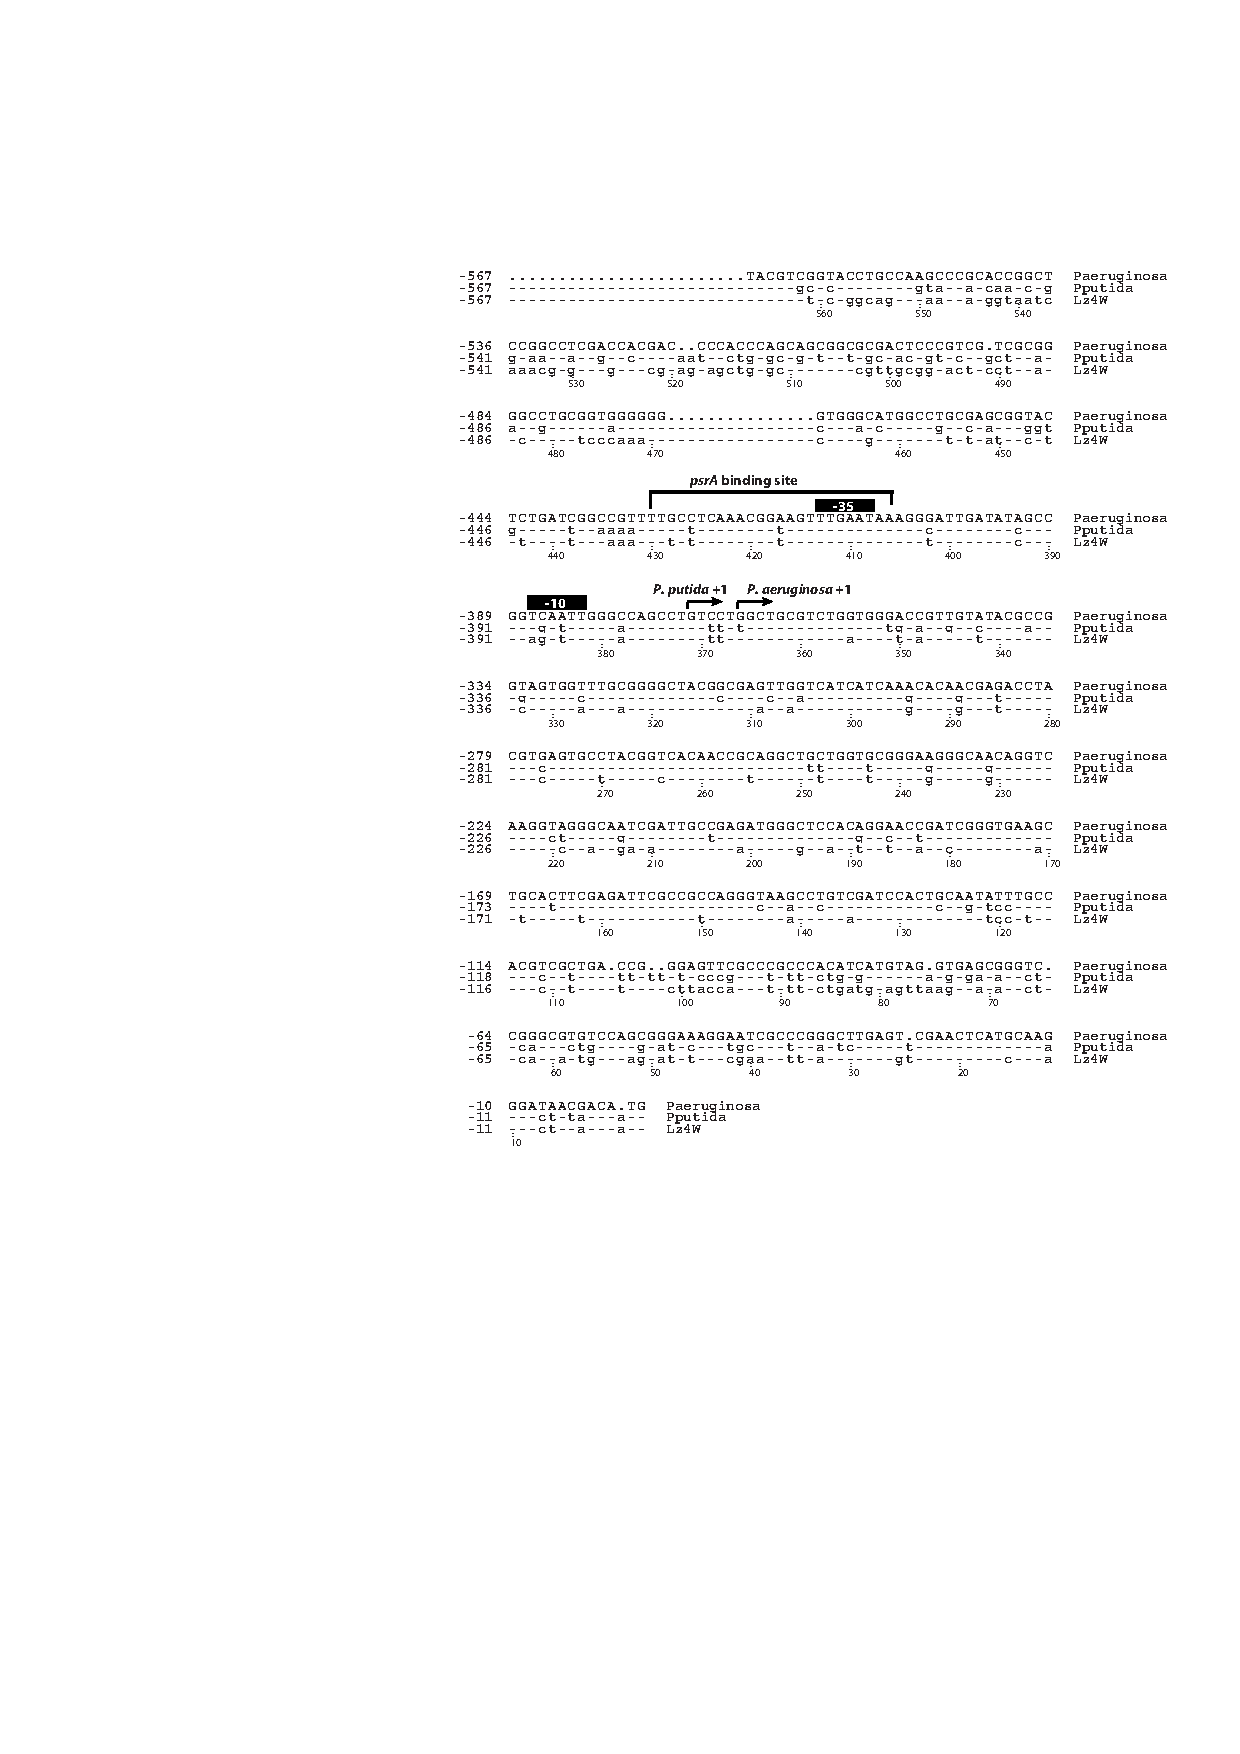
\includegraphics{figures/chap4_promoters}
\caption[Comparison of \e{rpoS} promoters]{Comparison of \e{rpoS}
promoters of Lz4W, \bact{Pa} (labelled as Paeruginosa), and \e{P.
putida} (labelled as Putida). The sequences are numbered
negatively in respect to translation initiation site. The
transcription start sites, $-$10, and $-$35 sites are indicated.
Gaps in the sequence are marked with dot and identical sequences
are marked with dash. The transcription start sites are taken from
\citet{Tanaka1994} for \bact{Pa} and \citet{Kojic2002} for \e{P.
putida}.} \label{chap4:promoters}
\end{figure}

\subsubsection{RNA secondary structure comparison}
\label{secondary} As discussed in Section~\ref{chap1:srna}, DsrA,
a small RNA (sRNA) in \bact{Ec}, binds to a stem-loop structure of
\e{rpoS} mRNA near the translation initiation region (TIR,
Figure~\ref{chap4:rna}A) and plays a major role in upregulation of
\sigs{} level at low
temperature~\citep{Lease2000,Lease2000b,Lease1998,Majdalani1998}.
A comparison of the secondary structures of TIRs of \e{rpoS} was
performed among \bact{Ec} and pseudomonad homologs
(Figure~\ref{chap4:rna}, to find out whether TIRs of pseudomonads
also form similar secondary structures.

\begin{sidewaysfigure}[tbp]
\centering
\includegraphics{figures/chap4_rna_structure}
\caption[RNA secondary structure comparison]{RNA secondary
structure comparison of the translation initiation regions of
\bact{Ec} \textbf{(A)}, Lz4W \textbf{(B)}, \e{P. putida}
\textbf{(C)}, and \bact{Pa} \textbf{(D)}\@. RNA sequence upstream
of the initiation codon (inclusive) to the transcription start
site were used for structure prediction by MFOLD version
3.1~\citep{Mathews1999}. Only the predicted lowest energy
structure of translation initiation region is shown in each case.
Putative ribosome binding sites are marked with red line,
initiation codon is colored blue, and the DsrA binding region in
\bact{Ec} structure is colored yellow. Note the numbering
increases towards the initiation codon.} \label{chap4:rna}
\end{sidewaysfigure}

The structures of the TIRs from \bact{Ec} and \bact{Pa}, although
very different in length (567 bases for \bact{Ec} and 366 bases
for \bact{Pa}), were strikingly similar. Both could potentially
form similar stem-loop structure involving ribosome binding site
(RBS), indicating both might be regulated by  similar mechanism. A
search in the genome sequence of \bact{Pa} with \bact{Ec} DsrA did
not find any significant hit. A search with the \bact{Pa}
stem-loop structure sequence ($-$229 to $-$242), however, returned
46 hits in the genome (data not shown). It remains to be seen
whether any of these hits are in fact DsrA homolog of \bact{Pa}.

TIRs of \e{P. putida} and Lz4W are, however, similar but different
from \bact{Ec} and \bact{Pa}. In first two instances, RBS is
almost completely buried within a stem (Figure~\ref{chap4:rna}B
and C), indicating a different regulation than that observed in
\bact{Ec} and \bact{Pa}.



\subsection{RpoS as phylogenetic tool}

Till date, outside of $\gammaup$ Proteobacteria, RpoS homologs
have been identified only in four species, three from $\betaup$
Proteobacteria and the other from \emph{Aquifex}. It is to be
noted that \emph{sigB} genes, in Gram positive bacteria, though
generally involved in stress response, are not homologs of RpoS.
From sequence alignnment, it is clear that all these three RpoS
sequences, obtained outside $\gammaup$ Proteobactaria are quite
diverged and can not be considered as RpoS homologs, unless
substantiated by biochemical and genetic data. It can therefore be
safely assumed that \emph{rpoS} gene is typically present only in
$\gammaup$ Proteobacteria.

\begin{figure}[tbp]
\begin{narrow}{-1.5in}{-1.5in}
\centering
\includegraphics{figures/chap4_dendrogram}
\end{narrow}
\caption[Phylogenetic tree of RpoS sequences]{Fitch-Margoliash
tree for RpoS sequences available in SwissProt/TrEMBL. The tree
was generated by the method of \citet{Fitch1967} from the multiple
sequence alignment depicted in Figure~\ref{rpos_align}. The
distances were calculated using PROTDIST program of PHYLIP
package~\citep{Fel1989}.} \label{tree}

\end{figure}

A Fitch-Margoliash tree from the alignment distinctly supports
this conclusion (Figure~\ref{tree}). Moreover, the tree also shows
the clustering of the three groups within $\gammaup$
Proteobacteria. According to the tree, \bact{Pa} RpoS is different
from the rest of the pseudomonads. It is to be noted that the same
conclusion could be derived from the comparison of the TIR
secondary structure comparison (Section~\ref{secondary}). As shown
in Figure~\ref{tree}, the closest sequence to \Lzsigs{} is RpoS
sequence from \e{P. tolaasii}.


\section{Discussion}

In this Chapter the results of the sequence comparison of RpoD and
RpoS sequences, currently present in the sequence database, have
been presented. Sequence comparison of RpoD showed that the
fragment of \Lzsiga{}, which has been cloned in the present study,
is highly similar to its mesophilic counterpart, and identical in
several of its keys residue positions. Particularly important was
region 2.3, which has been shown to initiate the melting of the
DNA strand during open complex formation. \Lzsiga{} was identical
in these residues to other mesophilic RpoD sequences. Moreover,
RpoD sequences from several of the known cold-adapted bacteria did
not show any significant deviation from the mesophilic sequence.
This finding, therefore, indicates that the specific regulator of
promoter melting during transcription at low temperature, if any,
is not located in  region 2.3, but might lie in region 1.1 of the
\s{} factor, which was missing from the cloned fragment.

Sequence comparison and phylogenetic analysis of RpoS revealed
that the gene is largely present of $\gammaup$ Proteobacteria.
Several of the key residues in RpoS are very similar to the
residues of RpoD. The comparison also revealed that the amber
mutation within RpoS reading frame would result in a \s{} factor
lacking region 4.1 and 4.2. This is important from the viewpoint
of a recent finding~\citep{Campbell2002} that the \bact{Ec} RpoD
without regions 4.1 and 4.2 could transcribe from promoters with
\emph{extended} $-$10 motif. As would be seen in the later
Chapters of this thesis, the truncated form of \Lzsigs{} is also
functional, and could transcribe from \bact{Ec} promoters with
\emph{extended} $-$10 like motif.

Promoter comparison with the other pseudomonads identified the
putative $-$10 and $-$35 promoters elements of \lzsig{}. The
binding site for the TetR family member PsrA were conserved in all
the pseudomonads sequences examined, including \lzsig{}. The
comparison also revealed that the putative $-$10 element of
\lzsig{} deviates from the consensus sequence.

RNA secondary structure comparison revealed that the translation
initiation region (TIR) of \lzsig{} differs from \bact{Pa} and
\bact{Ec}. As the secondary structure at TIR is important for
\e{rpoS} regulation, the different structure would predict a
different regulation of \lzsig{} than that in \bact{Ec} and
\bact{Pa}. \ding{45}


\FloatBarrier\pagebreak \thispagestyle{empty}
\begin{figure}[h]
\raggedleft
\includegraphics{figures/chap5_sep}
\end{figure}
\thispagestyle{empty}


\chapter{Effect of Lz4W \emph{rpoS} on \mbox{\emph{Escherichia coli}} promoters}

\section{Introduction}
\label{chap5:intro}

As discussed in the earlier chapters, \emph{rpoS} of Lz4W
(\emph{rpoS}\sub{Lz4W}) contains an amber mutation at codon 253 of
\emph{rpoS} reading frame. This is interesting from the view point
that several laboratory strains and natural isolates of \bact{Ec}
also harbor amber in
\emph{rpoS}~\citep{Jishage1997,Ivanova1992,Visick1997,Atlung2002}.
Furthermore, trehalose accumulation in these strains is dependent
on amber suppressor mutations~\citep{Rod1988}. Trehalose
accumulation in \bact{Ec} cells requires expression of
RpoS-controlled \emph{ots} gene~\citep{Hengge1991}. It is,
therefore, likely that amber suppression plays a crucial role in
expression of amber-mutated \emph{rpoS}\@. Moreover, these strains
exhibit variability in acid-sensitivity~\citep{Waterman1996}, and
in resistance to hydrostatic pressure \citep{Robey2001}. Similar
mutations in \emph{rpoS} have also been demonstrated in several
species of \emph{Salmonella}~\citep{Jorgensen2000,Sutton2000}.

Although, severely attenuated in RpoS-dependent stress-response,
many of these bacterial strains are not RpoS-null, even in the
absence of amber suppressor. There are several known mechanisms of
suppression of termination codon. Accumulating evidences indicate
that some of these even play regulatory roles in controlling gene
expression. Phenomena, such as, translational read-through,
frameshifting, and bypassing of the stop codon, occur even in
wild-type cells without any mutation in the translational
apparatus \citep{Hanna1996}. Su\-ch mechanisms play a very vital
role in bacteria (\emph{e.g.}, \emph{prfB} frameshifting in
\bact{Ec}), in viruses (\emph{e.g.}, capsid protein synthesis in
Q$\betaup$ phage) and have been proposed as a gene regulatory
mechanism in higher organism, such as, \emph{Drosophila}
\citep{Robinson1997}.

It has been demonstrated in earlier Chapters that the amber in
\lzsig{}, if not suppressed, would produce a $\sigmaup$, lacking
regions 4.1 and 4.2. Such a truncated \s{} would be intact upto
region 3.2. It is known that region 2 of $\sigmaup$\su{70} family
binds to $-$10 and region 4 binds to $-$35 elements of the
promoter. Remarkably, the region 4 of \siga{} in \bact{Ec} is
dispensable for promoters containing an \e{extended $-$10}
element~\citep[\seq{T\-G\-n\-T\-A\-T\-A\-A\-T},][]{Keilty1987,Kumar1993,Campbell2002}.
In fact, very recently, after elucidation of the crystal structure
of \emph{Thermus aquaticus} RNA polymerase, \citet{Campbell2002}
claimed that $\sigmaup$ region 1.2--3.1 contains all the elements
that are required for its function during transcription \e{in
vitro}.

In this Chapter, the ability of the \emph{rpoS}\sub{Lz4W} to
induce transcription from four known \emph{rpoS}-controlled
promoters of \bact{Ec} was examined. It was observed that \lzsig{}
in spite of lacking region 4, could activate a subset of promoters
in \emph{E. coli}. \lzsig{} was also tested for its ability to
complement catalase deficiency of a suppressor-containing
\bact{Ec} strain (JM101), where the indigenous \emph{rpoS} has
been mutated, to test the level to which suppressor tRNA can
suppress the amber mutation of \lzsig{}.

\section{Results}

Four known \emph{rpoS}-controlled promoters of \bact{Ec}, namely,
\emph{csiD}, \emph{bolAp1}, \emph{osmY}, and \emph{katE} were
tested by \emph{lacZ} genomic transcription fusion constructs. The
genomic copy of \emph{rpoS} in these strains was disrupted, and
the gene was provided on plasmid in \emph{trans}. To rule out any
inherent bias in cross-species complementation, \bact{Pa}
\emph{rpoS} (\emph{rpoS}\sub{Pa}) was taken as a positive control,
instead of native \bact{Ec} gene. All the complementation analyses
were carried out using high-copy-number plasmids. In case of
\lzsig{}, the plasmid vector was pBluescriptII KS+, and for
\emph{rpoS}\sub{Pa} it was pTZ18R. The effect of plasmid
copy-number, if any, was thought to be negligible by the fact that
both pBluescriptII KS+ and pTZ18R are high copy-number plasmids.
In plasmid p4C12 (contains \lzsig), the \emph{rpoS} was cloned in
the opposite direction to that of \emph{lacZ} promoter of the
vector to exclude its effect on the expression of \emph{rpoS}.


\subsection{Effect of Lz4W \emph{rpoS} on \emph{bolAp1}
promoter}

The \e{bolAp1} promoter in \bact{Ec} is regulated by \e{rpoS}. The
is responsible for the production of a \U{13}{kDa} morphogen in
the cell. To examine whether Lz4W \emph{rpoS} is capable of
activating \bact{Ec} \emph{bolAp1} promoter, p4C12 was introduced
into the strain ZK918~\citep[kind gift from R. Kolter. See
Table~\ref{ecolistrains} on page \pageref{ecolistrains} for
genotype]{Bohannon1991}. This strain was \emph{rpoS}-deficient due
to a deletional insertion generated by a \emph{rpoS}::Km fusion in
the genome. It also carried a chromosomal transcriptional fusion
of \emph{bolAp1} promoter to the \emph{lacZ}, at the \emph{bolA}
locus. Because \emph{bolAp1} promoter is \emph{rpoS} dependent,
the phenotype of the strain was reported to be RpoS\su{$-$}
LacZ\su{$-$} Km\su{r}~\citep{Bohannon1991,Ramos1998}. The
$\betaup$-galactosidase activities were measured in ZK918
containing p4C12 (\lzsig{}), ZK918 containing pDB18R (\pasig{};
positive control), and ZK918 containing pBluescriptII KS+ alone as
the negative control (Figure~\ref{chap5:zk918}).

\begin{figure}[tbp]
\begin{narrow}{-1in}{-1in}
\centering
\includegraphics{figures/chap5_zk918}
\end{narrow}
\caption[$\betaup$-galactosidase activity in transformed
ZK918]{$\betaup$-galactosidase activity in ZK918
(\emph{bolA}::\emph{lacZ} \emph{rpoS}) with growth phase, when
transformed with p4C12, containing Lz4W \emph{rpoS}. Plasmid
pDB18R, containing full-length \emph{rpoS} of \emph{P.
aeruginosa}, was taken as positive control and pBluescriptII KS+
was taken as plasmid control. X-axis shows the OD at 600 nm and
Y-axis shows $\betaup$-galactosidase activity in Miller units.}
\label{chap5:zk918}
\end{figure}

The $\betaup$-galactosidase activity of ZK918 containing p4C12 and
pDB18R were almost two-fold higher than the empty plasmid control,
along all the growth phases. While there was a peak of activity
for p4C12, at the early stationary phase (OD\sub{600} $\sim$1),
the activity decreased to the level observed in the presence of
\bact{Pa} \emph{rpoS} during the late stationary phase of growth.
This suggested that as shown in \bact{Ec}, the \e{bolAp1} promoter
is recognized and transcribed by both \lzsig{} and \pasig{} at the
stationary phase.

\subsection{Effect of Lz4W \emph{rpoS} on \emph{csiD} promoter}

The \e{csiD} is a carbon starvation induced gene in \bact{Ec} and
known be \e{rpoS}-controlled. The ability of \emph{rpoS}\sub{Lz4W}
to induce \emph{csiD} promoter was tested in the strain GJ2733
\citep[kind gift from J. Gowrishankar]{Rajkumari2001}, bearing an
operon fusion of \emph{csiD} promoter and \emph{lacZ}\@. The
indigenous \emph{rpoS} was disrupted in this strain by moving the
\emph{rpoS359}::Tn\emph{10} from RH90 \citep{Barth1995}. The
phenotype of the strain was reported to be LacZ\su{$-$},
RpoS\su{$-$}, Tc\su{r}~\citep{Rajkumari2001}. The production of
$\betaup$-galac\-to\-sidase was monitored in GJ2733 containing
\emph{rpoS}\sub{Lz4W} on p4C12, \pasig{} on pDB18R, and
pBluescriptII KS+ as empty plasmid control. There was a visible
difference of $\betaup$-galactosidase activities among these
strains on X-gal plate (Figure~\ref{chap5:csid_lacz}). The
$\betaup$-galactosidase activities of all these three strains were
also measured in LB broth in various growth phases
(Figure~\ref{chap5:csid_growth}). GJ2733 (p4C12) showed a marked
peak of $\betaup$-galac\-to\-sidase activity at late stationary
phase (OD\sub{600} $\sim$1.5). The activity increased from 30
units to 120 (Figure~\ref{chap5:csid_growth}B). The strain
containing plasmid pDB18R on the other hand showed a constant
level of expression at around 150 units throughout the growth
phases, as though the promoter remained at permanently derepressed
state of activation. The strain also grew very slowly than the
plasmid control and the strain containing p4C12
(Figure~\ref{chap5:csid_growth}A).

\begin{figure}[tbp]
\begin{narrow}{-1in}{-1in}
\centering
\includegraphics{figures/chap5_csid_lacz}
\end{narrow}
\caption[$\betaup$-galactosidase activity of GJ2733 on X-gal
plate]{$\betaup$-galactosidase activity of GJ2733 on X-gal plate
when transformed with p4C12 containing Lz4W \emph{rpoS}, pDB18R
containing \bact{Pa} \emph{rpoS} and pBluescriptII KS+.}
\label{chap5:csid_lacz}
\end{figure}





\begin{figure}[tbp]
\begin{narrow}{-1in}{-1in}
\centering
\includegraphics{figures/chap5_csid_lacz_graph}
\end{narrow}
\caption[$\betaup$-galatosidase activity in transformed
GJ2733]{$\betaup$-galactosidase activity in complemented GJ2733
(\emph{csiD}::\emph{lacZ} \emph{rpoS}) with growth phase, when
transformed with p4C12 containing Lz4W \emph{rpoS} ($\triangle$).
Plasmid pDB18R, containing full-length \emph{rpoS} of \bact{Pa}
($\medcirc$), was taken as positive control and pBluescriptII
KS+($\Box$) was taken as plasmid control. \textbf{(A)} The growth
of the 3 strains studied, represented as turbidity of the culture
measured as OD at \U{600}{nm}, plotted in Y-axis. X-axis shows the
time in hours. \textbf{(B)} $\betaup$-galactosidase activity,
measured as Miller units, plotted in Y-axis against OD at
\U{600}{nm} in X-axis.} \label{chap5:csid_growth}
\end{figure}

\subsection{Effect of Lz4W \emph{rpoS} on \emph{osmY}
promoter}

The \e{osmY} gene in \bact{Ec} is responsible for the production
of an osmotically induced periplasmic protein, and its promoter is
regulated by \e{rpoS}. The effect of \emph{rpoS}\sub{Lz4W} on
\bact{Ec} \emph{osmY} promoter was measured in GJ2734~\citep[kind
gift from J Gowrishankar]{Rajkumari2001}, which contains an operon
fusion of \emph{osmY} promoter and \emph{lacZ}. The indigenous
copy of \emph{rpoS} was mutated by moving
\emph{rpoS359}::Tn\emph{10} from RH90~\citep{Barth1995}. The
phenotype of the strain was reported to be RpoS\su{$-$},
LacZ\su{$-$} and Tc\su{r}. The strain was transformed with plasmid
p4C12 containing \emph{rpoS}\sub{Lz4W}, pDB18R, containing
\emph{rpoS}\sub{Pa} and pBluescriptII KS+ as empty plasmid
control. The result of the measured $\betaup$-galactosidase
activities at various phases of growth is shown in
Figure~\ref{chap5:osmy_growth}.

As shown in Figure~\ref{chap5:osmy_growth}A,
\emph{rpoS}\sub{Lz4W}-transformed GJ2734 grew slower than the same
strain containing \emph{rpoS}\sub{Pa} and empty plasmid. The
$\betaup$-galactosidase activities
(Figure~\ref{chap5:osmy_growth}B) remained essentially the same
throughout the growth phases (note the scale of Y-axis).

\begin{figure}[tbp]
\begin{narrow}{-1in}{-1in}
\centering
\includegraphics{figures/chap5_osmy_graph}
\end{narrow}
\caption[$\betaup$-galactosidase activity in complemented
GJ2734]{$\betaup$-galactosidase activity in complemented GJ2734
(\emph{osmY}::\emph{lacZ} \emph{rpoS}) with growth phase, when
transformed with p4C12 ($\medcirc$) containing Lz4W \emph{rpoS}\@.
Plasmid pDB18R ($\triangle$), containing \bact{Pa} \emph{rpoS} was
taken as a positive control and pBluescriptII KS+ ($\Box$) was
taken as plasmid control. \textbf{(A)} The growth of the three
strains studied, represented as turbidity of the culture measured
as OD at \U{600}{nm}, plotted in Y-axis. X-axis shows the time in
hours. \textbf{(B)} $\betaup$-galactosidase activity, measured as
Miller units plotted in Y-axis against OD at \U{600}{nm} in
X-axis.} \label{chap5:osmy_growth}
\end{figure}

\subsection{Effect of Lz4W \emph{rpoS} on \emph{katE}
promoter} \label{chap5:kate}

In a similar study on the effect of \emph{rpoS}\sub{Lz4W} on
\emph{katE} (encoding stationary phase specific catalase HPII)
promoter in \bact{Ec} it was found that there was no difference of
$\betaup$-galactosidase activities amongst strains harboring
p4C12, pDB18R, and pBluescriptII KS+. The activities were measured
in GJ2782~\citep[kind gift from J Gowrishankar]{Rajkumari2002},
which contains \emph{katE}::\emph{lacZ} fusion at the $\lambdaup$
integration site. The strain was derived from
RH100~\citep{Hengge1993}, where the \emph{nlpD}--\emph{rpoS}
region were deleted from the chromosome. The
\emph{katE}::\emph{lacZ} from strain KT1008EL~\citep{Tanaka1997}
was moved into RH100. The phenotype of the strain was reported to
be RpoS\su{$-$}, LacZ\su{$-$} and Km\su{r}. This strain, when
transformed with p4C12, pDB18R, and pBluescriptII KS+, the
$\betaup$-galactosidase activities in all these three remained
constant around 1--5 units throughout the growth phase (data not
shown). Surprisingly, even pDB18R failed to restore activity,
indicating that \emph{katE} is probably not recognized at all by
\bact{Pa} \emph{rpoS}.

\subsection{Effect of amber-suppressor \emph{supE} on Lz4W \emph{rpoS}}

The results of the \e{lacZ} expression studies described above
indicated that the \lzsig{} could probably transcribe from atleast
two of the four \sigs{}-controlled promoters in \bact{Ec}. To
examine whether this expression is due to to a suppression of the
amber, the stationary phase specific catalase activity was assayed
in an \bact{Ec} strain bearing a known suppressor (JM101).

%We wanted to find out whether the amber in \lzsig{} can be
%suppressed by a known suppressor in \bact{Ec}. We chose catalase
%as a marker. As discussed in Section~\ref{chap5:kate}, promoter of
%\emph{KatE}, coding for HPII catalase is not affected by
%\emph{rpoS}\sub{Lz4W}. We tested the ability of a background
%amber-suppressor to restore back the \emph{KatE} promoter activity
%by \emph{rpoS}\sub{Lz4W}.

In \emph{E. coli}, there are two catalases known. Catalase HPI,
coded by \emph{katG} and HPII, coded by \emph{katE}. There is now
considerable evidence that both these genes are controlled by
\emph{rpoS}\@. In RpoS\su{$-$} mutant, the catalase levels are
poor and the RpoS\su{$+$} and RpoS\su{$-$} strains can be easily
distinguished by a simple H\sub{2}O\sub{2} bubbling test, where
dropping of H\sub{2}O\sub{2} directly on a colony will from
bubbling due to break down of H\sub{2}O\sub{2} by cellular
catalase~\citep{Mulvey1988}.

JM101, which contained \emph{supE}, a known amber-suppressor, was
made RpoS\su{$-$} by P1 transduction, by moving
\emph{rpoS359}::Tn\emph{10} allele from Rh90 (see Sections
\ref{rh90_lysate} and \ref{P1_transduction} on page
\pageref{P1_transduction} for datails). The resulting strain
named, MJMRH is RpoS\su{$-$}, Catalase\su{$-$}, Tc\su{r} and
\emph{supE}\@. This strain was then transformed with plasmid p4C12
containing \emph{rpoS}\sub{Lz4W}, pDB18R containing
\emph{rpoS}\sub{Pa} as positive control, and pBluescriptII KS+ as
plasmid control. The H\sub{2}O\sub{2} bubbling test was performed
on these three strains (Figure~\ref{chap5:jm101}).

\begin{figure}[tbp]
\centering
\includegraphics{figures/chap5_jm101}
\caption[H\subsf{2}O\subsf{2} bubbling test on complemented
MJMRH]{H\subsf{2}O\subsf{2} bubbling test on MJMRH transformed
with p4C12 containing Lz4W \emph{rpoS}, pDB18R containing
\bact{Pa} \e{rpoS}, and pBluescriptII KS+ as plasmid control. The
transformed plasmid in each case is labelled on top.}
\label{chap5:jm101}
\end{figure}

MJMRH expectedly, had very little catalase activity when
transformed with empty plasmid (track marked as pBluescriptII KS+
in Figure~\ref{chap5:jm101}). Cells transformed with pDB\-18R
(track marked as pDB18R in Figure~\ref{chap5:jm101}) exhibited
very high activity. The activity was intermediate in cells
transformed with p4C12 (track marked as p4C12 in
Figure~\ref{chap5:jm101}). Although, pDB18R and p4C12 could not
activate transcription from \emph{katE} promoter, MJMRH showed a
marked increase in catalase activity, when transformed with
pDB18R. Possibly, both p4C12 and pDB18R induced transcription
through an unknown mechanism, through an indirect effect on
\emph{katE}, or by their effect on \emph{katG}, encoding HPI
catalase.

\subsection{Comparison of \emph{rpoS}-controlled promoters of
\bact{Ec}}

In an attempt to explain why \emph{csiD} and \emph{bolAp1}
promoters were activated by \lzsig{} while \emph{osmY} and
\emph{katE} remained unaffected, promoter sequences from 49
\bact{Ec} genes known to get transcribed by \sigs{}, were compared
(Figure~\ref{chap5:promoter_comparison}). Remarkably, both
\emph{csiD} and \emph{bolAp1} had \seq{G} at $-$14, whereas,
\emph{osmY} and \emph{katE} had \seq{T} and \seq{C}, respectively,
at this position. A search for \seq{G} at $-$14 of various
\sigs{}-controlled promoters in \bact{Ec} showed that it is
present only in \emph{ada}, \emph{dnaQp2}, \emph{dps},
\emph{galp1}, \emph{gor}, \emph{osmBp2}, \emph{pqi5p2},
\emph{proPp2}, \emph{rnaI}, \emph{topA}, and \emph{xthA} promoters
(underlined promoters in Figure~\ref{chap5:promoter_comparison}).
\seq{G} at $-$14 is known to enhance transcription both by \siga{}
and \sigs{} (see Section~\ref{chap5:discussion}). Moreover,
extended $-$10 promoters which are known to get transcribed by
\bact{Ec} \siga{} without region 4, has \seq{G} at $-$14. It is,
therefore, possible that \lzsig{} can activate transcription, in
spite of lacking region 4.

\begin{figure}
\centering
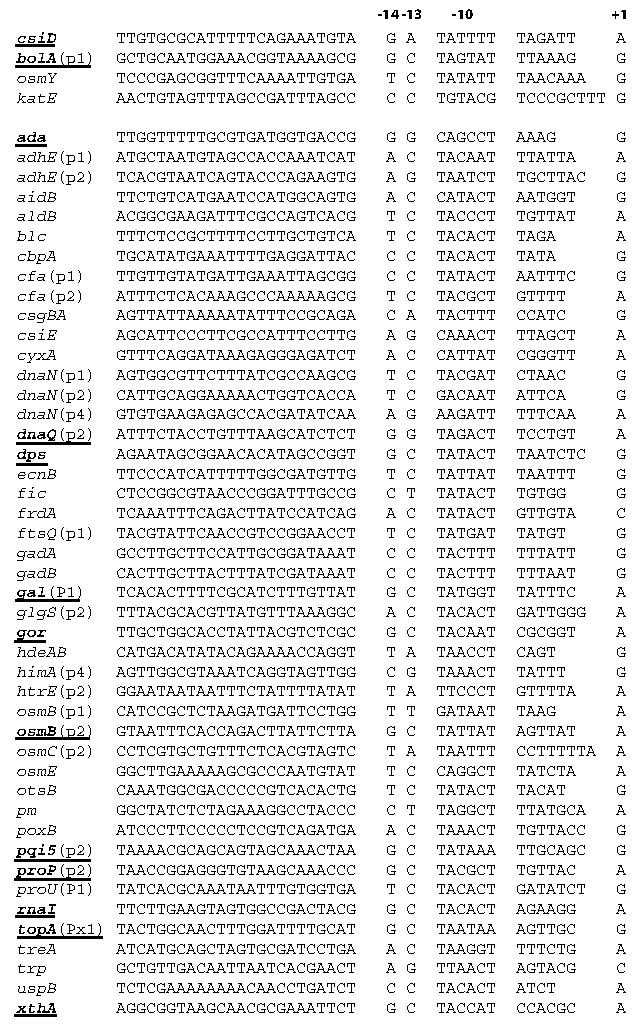
\includegraphics{figures/chap5_promoter_align}
\caption[Comparison of \emph{rpoS}-controlled promoter of \emph{E.
coli}]{Comparison of known \emph{rpoS}-controlled promoters of
\bact{Ec}. The sequences were gathered from various sources,
hand-aligned, and rearranged after \citet{Becker2001} to show
corresponding elements of promoters recognized by
$\sigmaup$\smallsu{70}. The promoters with G at position -14 are
underlined and in bold font. The transcription start site, $-$10,
$-$13, and $-$14 sites are indicated on top. The first four
promoters, separated from the rest by blank line, are tested in
this study.} \label{chap5:promoter_comparison}
\end{figure}


\section{Discussion}
\label{chap5:discussion}

The studies in this Chapter were carried out to examine whether
\lzsig{} could transcribe from known \bact{Ec}
\emph{rpoS}-con\-trolled promoters \e{in vivo}. Although, it
harbors an amber in its reading frame, \emph{rpoS}\sub{Lz4W} could
induce transcription from two (\emph{csiD} and \emph{bolAp1}) out
of four tested promoters.

There are contradictory reports regarding the ability of
\emph{Pseudomonas rpoS} to induce \bact{Ec} promoters. \bact{Pa}
\emph{rpoS} that was used in this study was reported to be able to
restore the catalase deficiency of \bact{Ec} \emph{rpoS}
mutant~\citep{Tanaka1994}. In a later study, however, the same
group could not detect any transcript of the same gene when
transformed in \bact{Ec}~\citep{Fujita1994}. In this study, it was
observed that \emph{rpoS}\sub{Pa} had marginal effect on
\emph{bolAp1} and no effect on \emph{osmY}\@. The \emph{csiD}
promoter, however, was activated by \pasig{} in all the growth
phases. The induction during the entry into stationary-phase, a
feature of \emph{rpoS}-controlled promoters, was distinctly
absent. It indeed restored the catalase activity in RpoS$^{-}$
cells, but obviously, not through a direct effect on
\emph{katE}\@. It also affected the growth rate of transformed
cells, but the effect was too variable to reach to any conclusion.

The pattern of induction by \lzsig{}, on the other hand,  shows
the characteristic peak of \emph{rpoS}-dependent \e{lacZ} activity
at the stationary phase for both \emph{bolAp1} and \emph{csiD}
promoters, even though it harbors an amber in the reading frame.
The induction was five folds for \emph{csiD} but only two folds
for \emph{bolAp1}. \emph{osmY} and \emph{katE} promoters were not
affected at all. As these promoters were not affected even by
\pasig{}, it is reasonable to state that \emph{Pseudomonas}
\emph{rpoS} can not activate \emph{osmY} and \emph{katE} promoters
of \bact{Ec}. Based on the results presented in this Chapter, it
can also be suggested that the amber in \lzsig{} is not
efficiently be suppressed by a known amber suppressor
(\emph{supE}) of \bact{Ec}.

The striking effect of \lzsig{} was observed on \emph{csiD}
promoter, where it activated the promoter almost to the level of
native \bact{Ec} gene. There could be two mechanisms by which
\lzsig{} could induce any promoter. First, the truncated protein
produced due to amber itself could be functional, or second, the
amber mutation is overcome by a read-through or by an
amber-suppression. Two strains where it induced transcription were
not reported to carry any amber suppressor; moreover, even
introduction of an exogenous suppressor allele could not
significantly restore its effect on transcription. Thus the
possibility of an suppressor mutation suppressing this amber was
less likely.

There is, however, exists a possibility that a read-through
full-length RpoS is produced which induced these promoters. The
existing data are not sufficient to discard this possibility.
There was an earlier report that the C-terminal 16 amino-acids are
important for \bact{Ec} RpoS activity on \emph{katE}, \emph{fic}
and \emph{bolA} promoters~\citep{Ohnuma2000}. In contrary, Lz4W
\emph{rpoS}, which lacks C-terminal entirely, could activate
\emph{bolA}, albeit, only two folds (Figure~\ref{chap5:zk918}).

Therefore, could it be possible that \lzsig{} is functional even
without region 4? In fact, it is now known that at least \siga{},
lacking region 4, can transcribe promoters with an \e{extended
$-$10}~\citep[\seq{T\-G\-n\-T\-A\-T\-A\-A\-T},][]{Keilty1987,Kumar1993,Campbell2002}\@.
\seq{TG} motif at $-$15 and $-$14 has been shown to be present in
25\% of all \bact{Ec} promoters~\citep{Burr2000}. Identical
mechanism could be operational for \sigs{}. The argument for this
possibility is threefold:

\begin{enumerate}

\item \siga{} and \sigs of \bact{Ec} are highly similar in their
recognition features at $-$10 of the promoters~\citep{Lee2001}.
Several \bact{Ec} promoters were found to be recognized by both
the $\sigmaup$ factors \emph{in
vitro}~\citep{Tanaka1993,Tanaka1995}. Selection experiments
(SELEX), performed \emph{in vitro} with \bact{Ec} \sigs{} selects
promoter sequence identical to that of \siga{}~\citep{Gaal2001}.
Both these $\sigmaup$ factors have almost identical sequences, in
the crucial functional regions~\citep{Lonetto1992,Gruber1997}.


\item Interaction between extended $-10$ with region 3.0 of
$\sigmaup$ has been well documented for both \siga{} and
\sigs{}~\citep{Voskuil1995,
Barne1997,Becker1999,Colland1999,Burr2000,Becker2001}.
Particularly important is \seq{G} at $-14$,  which has been shown
to have an activating effect on both \siga{}~\citep{Barne1997} and
\sigs{}~\citep{Becker2001}. We have also shown that both the
\lzsig{}-affected promoters, \emph{bolAp1} and \emph{csiD} have
\seq{G} at $-$14.

\item Moreover, experiments done with \emph{fic} promoter, which
does not use $-$35 contact at all~\citep{Tanaka1995}, and with
point mutations isolated in \emph{osmE}
promoter~\citep{Bordes2000}, as well as compilations of promoter
sequences~\citep{Espinosa1996} indicate that \sigs-dependent
promoters have weak or no $-$35 regions~\citep{Becker2001}.
Recognition of $-$35 element is, therefore, of less importance for
\sigs.

\end{enumerate}

It is, therefore, can be predicted that like \siga{}, \sigs{}
could function without region 4 for promoters with extended $-$10.
And it is probable that \lzsig{} can activate promoter with
extended $-$10 in spite of lacking region 4. It has been shown
that only a subset of \emph{rpoS}-controlled promoters that has
\seq{G} at $-$14 are potential candidate to get affected by
\lzsig{}, resulting in promoter discrimination within \emph{rpoS}
regulon. The implication of such discrimination, if at all
operational in Lz4W, remains to be investigated.\ding{45}


\FloatBarrier\pagebreak \thispagestyle{empty}
\begin{figure}[h]
\raggedleft
\includegraphics{figures/chap6_sep}
\end{figure}
\thispagestyle{empty}


\chapter{Phenotypic and Molecular Characterization of \emph{rpoS} from \e{Pseudomonas syringae} Lz4W}

\section{Introduction}
\label{chap6:intro} In previous Chapters it was shown that
\lzsig{} harbors an amber mutation in its reading-frame which
could potentially produce a truncated, yet functional RpoS, at
least as far as the induction of \bact{Ec} promoters is concerned.
It were demonstrated in several studies that \emph{rpoS}, in a
wide range of bacterial species, is prone to mutation.
Interestingly, it was also observed that the stationary phase
cultures of \bact{Ec} are easily taken over by mutants that have
selective advantage over the ancestral
population~\citep{Zambrano1993}. These mutants, aptly termed as
``GASP'' (\emph{G}rowth \emph{A}dvantage in \emph{S}tationary
\emph{P}hase), are able to grow when the ancestral population can
not. These GASP mutants, apparently, are able to reinitiate growth
by scavenging nutrients released by dying
cells~\citep{Zinser1999}. In fact, multiple rounds of mutants
arise to take over the ancestral population during prolonged
starvation~\citep{Finkel1999}. Although, GASP mutations are of
different kinds, some involved in amino acid
catabolism~\citep{Zinser1999}, some are in transcription factor
such as \emph{lrp}~\citep{Zinser2000}, the striking fact is that
the first round of mutations that take over the culture, are more
often than not located in \emph{rpoS}~\citep{Vulic2001}.

Given, that \emph{rpoS} controls the general stress response in
\bact{Ec} and related bacteria, and influence the survivality at
stationary phase, GASP mutants creates a paradox in the field.
This apparent paradox was addressed in a recent study where it was
shown that \emph{rpoS} mutation has a selective advantage during
slow growth in chemostat culture of \bact{Ec}~\citep{Mcrobb2002}.
It was proposed that \emph{rpoS} mutation causes an upregulation
of \emph{rpoD} controlled genes, which confers a selective
advantage through increase in outer membrane permeability and
increased nutrient scavenging under low nutrient
conditions~\citep{Mcrobb2002}. Interestingly, in conditions of
dual stress, like low pH and carbon starvation, majority of the
\emph{rpoS} GASP mutations are not null but attenuated
\emph{rpoS}, containing amber. This observation led the authors to
conclude that amber mutation in \emph{rpoS} is a mechanism to
reduce, at the same time maintaining enough \emph{rpoS} activity
to cope with the stress condition, such as low pH.

Low temperature is one of the known stress conditions that
increases RpoS level in \bact{Ec}. In \bact{Ec}, RpoS protein is
unstable and is present only in small amounts during exponential
growth at 37\dg{}~\citep{Lange1994}. The level of RpoS, however,
increases during exponential growth at low temperature (20\dg{}),
mediated by a 87 nucleotide long RNA, DsrA~\citep{Sledjeski1996}.
DsrA functions through an \emph{anti-anti-sense} mechanism that
disrupts intramolecular basepairing in \emph{rpoS} mRNA,
facilitating \emph{rpoS} translation at low
temperature~\citep{Majdalani1998,Lease1998,Lease2000}.

Upregulation of the \emph{rpoS} was  reflected in upregulation of
several \emph{rpoS}-controlled promoters at low temperature,
measured using \emph{lacZ}
fusions~\citep{Sledjeski1996,Rajkumari2001}. The role of
\emph{rpoS} in growth at low temperature, however, remains
elusive. \emph{rpoS} mutant, grew as fast as the wild-type cells
at low temperature~\citep{Sledjeski1996}.

Contrary to its role during growth at low temperature, the role of
\emph{rpoS} in other stress conditions are well defined. Two of
the several stress responses where \emph{rpoS} plays a crucial
role are, acid stress and oxidative stress. Although, the
mechanism is not clearly understood, \emph{rpoS}-dependent
acid-tolerance in \bact{Ec} and related bacteria is well
documented~\citep{Small1994,Cheville1996,Lee1995}. Acid
sensitivity of \emph{rpoS} mutants has been shown in a wide range
of bacterial species, including
\emph{Pseudomonas}~\citep{Jorgensen1999}.

The underlying mechanism, how cells cope with oxidative stress in
\emph{rpoS}-dependent manner is well understood in \bact{Ec}. The
bacterium is known to possess two catalases, HPI, encoded by
\emph{katG}, and HPII encoded by \emph{KatE}\@. HPI is a
hydroperoxidase, tetramer of \U{80,049}{Da} subunits, induced by
H\sub{2}O\sub{2} and associated with the plasma membrane in
\bact{Ec}~\citep{Schellhorn1995,Heimberger1988,Loewen1985}. The
induction of \emph{katG} by H\sub{2}O\sub{2} is mediated through
OxyR, which directly senses the oxidative stress and is activated
by conformational change upon oxidation occurring at a key
cysteine residue~\citep{Storz1990}. HPII hydroperoxidase, on the
otherhand, is a hexamer of \U{93,000}{Da} subunits and mainly
restricted to cytoplasm
\citep{Schellhorn1995,Heimberger1988,Loewen1985,Loewen1986,Loewen1984a}.
HPII level increases 10--20 folds during entry into stationary
phase but it is not induced by H\sub{2}O\sub{2}. \emph{katE}, the
gene encoding HPII was found to be controlled by \emph{rpoS}. In
fact, one of the first phenotypes identified for \emph{rpoS} was
severe catalase deficiency of \emph{rpoS} mutant, and \emph{rpoS}
was therefore, named as \emph{katF}~\citep{Loewen1984b}.

There is, however, contradictory reports about the role of
\emph{rpoS} in HPI expression. While an earlier report suggested a
\emph{rpoS}-dependent increase of \emph{katG} activity during
stationary phase~\citep{Ivanova1994}, a later report showed that
the increase of HPI level is not dependent on
\emph{rpoS}~\citep{Visick1997}. Moreover, in \emph{rpoS} mutant,
there was an increase in HPI expression, more than the expression
in isogenic wild type cell~\citep{Visick1997}.

\bact{Ec} catalases, however, are different from their counterpart
in other species. Even within Enterobacteriaceae, there is a wide
variation in catalsases~\citep{Switala1990}. Three distinct
catalase isozymes were reported in \emph{Bacillus
subtilis}~\citep{Loewen1987}. Within \emph{Pseudomonas}, catalases
vary greatly, in some instances even within same species. For
example, number of catalases vary from two in case of \emph{P.
syringae} pv. phaseolicola to eight in case of \emph{P. syringae}
pv. glycinea~\citep{Klotz1992}. In \bact{Pa} there are two
catalsases, \emph{katA} and \emph{katB}. Both these genes are
induced by H\sub{2}O\sub{2} and
OxyR~\citep{Ochsner2000,Hassett2000,Fredrick2001}. Catalase
production was found to be 60\% lower in \emph{rpoS} mutant of
\bact{Pa}~\citep{Suh1999}. The only known \emph{Pseudomonas}, that
comes closest to \bact{Ec} in terms of the numbers of catalases
present and their expression profile, is perhaps, \emph{P. putida}
mt-2, where \emph{katA} and \emph{katB} behaves like HPI and HPII
of \bact{Ec}~\citep{Miura1998}.

The experiments described in this Chapter were conducted to
address the role of \lzsig{} in cold adaptation and associated
stress response of Lz4W. The level of RpoS was compared in
immunoblot under various growth conditions. The amber mutation in
\lzsig{} reading frame resulted in a truncated protein of
\U{31}{kDa}. There was a distinct suppression of RpoS during
growth of Lz4W at low temperature. The null-mutant of \e{rpoS},
generated by insertional inactivation of \e{rpoS}, was compared
with the wild-type for its growth and stress tolerance at
different temperatues. \emph{rpoS} mutant of Lz4W was marginally
cold sensitive and acid-sensitive, both at high and low
temperature. This indicated that the truncated RpoS in Lz4W was
indeed functional. It was also observed that Lz4W had only one
isozyme of catalase, whose expression was growth phase dependent.
The expression became uncontrolled, even marginally higher in
\emph{rpoS} mutant. Finally, to address the question, whether the
amber mutation in \lzsig{} confers any selective advantage during
growth under various conditions, the mutation was corrected to
obtain a full-length \e{rpoS}. The corrected protein was
constructed by joining the N-terminal half of \lzsig{} and
C-terminal half from \pasig{}. This full-length RpoS caused severe
growth retardation in cold (4\dg{}), thus indicating that amber
mutation in \lzsig{} might have a growth advantage at low
temperature and possibly has been selected during cold-adaptation
of the bacterium in Antarctica.

\section{Results}

\subsection[RpoS expression]{Growth-phase and temperature-dependant RpoS expression}
\label{chap6:rpos_expression}

RpoS protein level was compared along the growth stages of Lz4W
cells at 22\dg{} and at 4\dg{}, in a semi-quantitative immunoblot
analysis. A mouse anti-RpoS polyclonal anti-serum~\citep[kind gift
from M. Kivisaar]{Ojangu2000}, generated against the \sigs{} of
\bact{Pp} was used in all immunoblot analyses. When used in the
present study, a rabbit anti-serum against \bact{Ec} RpoS (kind
gift from R. Hengge-Aronis) did not give consistent results (data
not shown). The experiments were carried out as described in
Section~\ref{mat:immunoblot}.

Briefly, aliqouts of Lz4W cultures growing at steady-state at
22\dg{} and at 4\dg{} were collected at mid-log phase (OD\sub{600}
$\sim$0.5), late-log phase (OD\sub{600} $\sim$1),
early-sta\-tionary phase (OD\sub{600} $\sim$1.5), and
stationary-phase (OD\sub{600} $\sim$1.7--1.8) of the growth
(Figure~\ref{chap6_rpos_western}A). Equal amount of proteins from
each of these samples were analyzed in immunoblot using anti-RpoS
antibody. Two bands were detected, one of \U{$\sim$31}{kDa} and
another of \U{$\sim$20}{kDa} (arrows in
Figure~\ref{chap6_rpos_western}B). Although, the expected size of
truncated RpoS (because of the presence of amber) was
\U{$\sim$29}{kDa}, it can be assumed that the \U{$\sim$31}{kDa}
band was the truncated product, as RpoS is known to exhibit
anomalous mobility in SDS-PAGE. The lower band (\U{20}{kDa}) was
possibly a degradation product of RpoS. No other bands of size
\U{>31}{kDa} was detected, indicating that amber in RpoS reading
frame in Lz4W was not suppressed, atleast to the level detectable
in immunoblots.

\begin{figure}[tbp]
\begin{narrow}{-1in}{-0.6in}
\flushright
\includegraphics{figures/chap6_rpos_western_points_removed}
\end{narrow}
\caption[Growth-temperature dependant RpoS
expression]{Growth-temperature dependant RpoS expression.
\textbf{(A)} A representative growth curve of Lz4W at 22\dg{}
(solid line) and at 4\dg{} (dotted line). The growth stages of
sample collection for immunoblotting are indicated by arrows.
\textbf{(B)} Semi-quantitative immunoblot showing RpoS expression
along the growth stages in two different temperatures. The
temperatures and the OD\sub{600} for each samples are indicated on
top. Molecular weight markers in kDa are indicated on right. The
two prominent RpoS bands are indicated by arrows on left.
\textbf{(C)} Ponceau S stained blot indicating equal loading of
each samples. \textbf{(D)} Densities of the RpoS
(\U{$\sim$31}{kDa}) bands in arbitrary units measured by image
analysis. Filled bars ($\blacksquare$) and open bars ($\square$)
represent samples from cells grown at 22\dg{} and 4\dg{},
respectively.} \label{chap6_rpos_western}
\end{figure}

There was a characteristic increase in the RpoS protein level
along the grow\-th phases in Lz4W cells, both when grown at
22\dg{} (first four lanes from left to right in
Figure~\ref{chap6_rpos_western}B) and at 4\dg{} (last four lanes
from left to right in Figure~\ref{chap6_rpos_western}B).
Expectedly, RpoS level increased during entry into
stationary-phase. The increase was eight folds in cells grown at
22\dg{} (filled bars in Figure~\ref{chap6_rpos_western}D), but
only four folds when grown at 4\dg{} (open bars in
Figure~\ref{chap6_rpos_western}D). When RpoS levels at 22\dg{} and
4\dg{} were compared, it was found that the level of RpoS was less
than 50\% in cells grown at 4\dg{} to the level found in cells
grown at 22\dg{}\@. The difference was maximum at stationary-phase
(Figure~\ref{chap6_rpos_western}D). At mid-log phase (OD\sub{600}
0.5), cells from both the temperatures had comparable levels of
RpoS but when they progressed towards stationary phase the
difference became pronounced (Figure~\ref{chap6_rpos_western}D).


\subsection{Construction of a \emph{rpoS} disruption mutant}

A disruption mutant of Lz4W \emph{rpoS} was created by homologous
recombination as described in Section~\ref{chap2_disrupt} on page
\pageref{chap2_disrupt} and depicted in
Figure~\ref{chap6_rpos_disruption}. The gene was disrupted before
the amber to generate a null-mutant.



\begin{sidewaysfigure}[tbp]
\centering
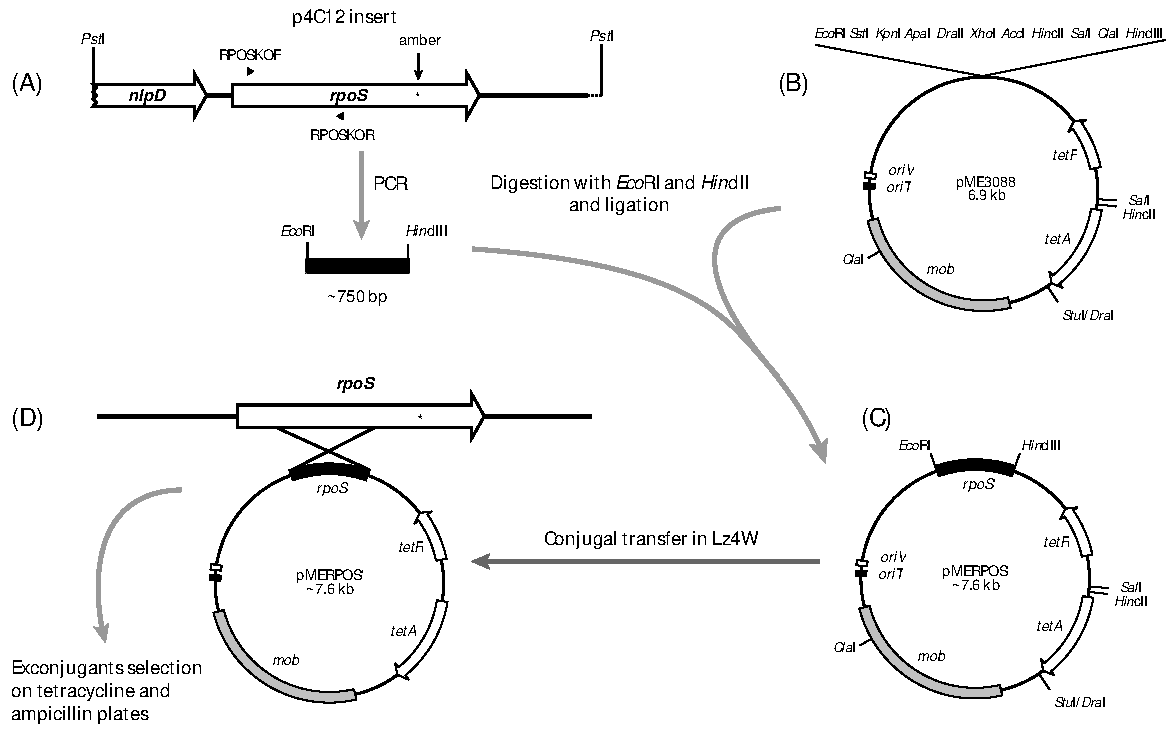
\includegraphics{figures/chap6_knock_out}
\caption[Generation of \emph{rpoS} disruption mutant]{Generation
of \emph{rpoS} disruption mutant of Lz4W. \textbf{(A)} An internal
fragment of 753 bp, before the amber mutation of the \emph{rpoS}
gene was amplified using PCR. The positions of the primers RPOSKOF
containing \emph{Eco}RI site and RPOSKOR containing \emph{Hin}dIII
site are indicated by arrow-heads\@. \emph{rpoS} and upstream
\emph{nlpD} reading frames are indicated by open arrow. The
position of the amber is shown by ``$\ast$''. \textbf{(B)} The map
of the suicide vector pME3088 with Tc\su{r} marker. \textbf{(C)}
The amplified PCR fragment was cloned into pME3088 at \emph{Eco}RI
and \emph{Hin}dIII sites. The resulting plasmid is called
pMERPOS'. \textbf{(D)} pMERPOS' was transferred into Lz4W by
conjugation. A single recombination event would knock-out
\emph{rpoS} with the integration of the whole plasmid into the
genome. The exconjugants were selected on tetracycline and
ampicillin plates. Note that the recombination event would disrupt
the reading frame before the amber.} \label{chap6_rpos_disruption}
\end{sidewaysfigure}


The strategy of \emph{rpoS} disruption relied on a single
recombination event with plasmid pMERPOS$'$ with the genomic copy
of \emph{rpoS} (Figure~\ref{chap6_rpos_disruption}D)\@. It is to
be noted that a single recombination event would result in the
integration of the whole plasmid (pMERPOS$'$) into the genome.
pMERPOS$'$ was derived from suicide vector
pME3088~\citep[Figure~\ref{chap6_rpos_disruption}B]{Schnider2000},
which lacks \emph{Pst}I site in the vector backbone. As it was
shown earlier, the insert in p4C12 detected a \U{$\sim$2.1}{kb}
\emph{rpoS} band in \emph{Pst}I digested genomic DNA from Lz4W.
Whether or not the whole pMERPOS$'$ integrated into the
\emph{rpoS} gene, could, therefore, be easily verified by probing
\emph{Pst}I digested genomic DNA with insert from plasmid p4C12.
In the disrupted strains the insert from p4C12 should detect a
band of \U{$\sim$9.7}{kb} (\U{7.6}{kb} of pMERPOS$'$ plus
\U{2.1}{kb} of genomic copy of \emph{rpoS}).


\begin{figure}[tbp]
\centering
\includegraphics{figures/chap6_mutant_southern}
\caption[Construction of \e{rpoS} disruption mutant]{Construction
of Lz4W \emph{rpoS} disruption mutant. Four randomly selected
exconjugants from the disruption scheme described in
Section~\ref{chap2_disrupt} and in
Figure~\ref{chap6_rpos_disruption} was tested for the presence of
RpoS protein in immunoblot and in genomic Southern blot. The
strains used are indicated on top and the lane numbers are marked
in bottom. \textbf{(A)} Immunoblot showing the absence of the RpoS
bands in mutants (lanes 2--5). The RpoS band in the wild type (WT)
Lz4W (lane 1) is marked with an arrow. \textbf{(B)} Southern blot
analysis using \emph{Pst}I-digested genomic DNA isolated from the
mutants (lanes 2--5) and wild type Lz4W (lane 1), probed with
insert of plasmid p4C12, spanning the full-length \emph{rpoS} of
Lz4W. The \emph{rpoS} band in wild type Lz4W is marked with an
arrow. Numbers on the right show the marker positions in
base-pairs. Note the single insertion in MBLz4W.}
\label{chap6:mutant_southern}
\end{figure}

In order to verify this, the genomic DNA, isolated from four
putative mutants were digested with \emph{Pst}I and probed with
the insert of p4C12 (Figure~\ref{chap6:mutant_southern}B)\@. All
these four mutants (lanes 2--5 in
Figure~\ref{chap6:mutant_southern}B) displayed the expected
\U{$\sim$9.6}{kb} band, thus, confirming that pMERPOS$'$ indeed
had been integrated into the genome at \emph{rpoS} locus in these
mutants. It is to be noted that mutant 4 had only a single
insertion in the genome, represented by single band, whereas
mutants 1--3 had multiple insertions, represented by multiple
bands. The mutant 4 was named MBLz4W and  was used for all further
studies.

The inactivation of \e{rpoS} gene in the four randomly selected
null-mutants were also verified for the absence of the RpoS
protein by immunoblot analysis
(Figure~\ref{chap6:mutant_southern}A)\@. All these four clones
(lanes 2--5 in Figure~\ref{chap6:mutant_southern}A) were negative
for RpoS protein, confirming their RpoS-null phenotype.


\subsection{Lz4W \emph{rpoS} null-mutant is marginally cold-sensitive}

The ability of the \e{rpoS} null-mutant, MBLz4W to grow at 4\dg{}
was examined to verify the importance of \e{rpoS} during growth at
low temperature. On ABM agar plate, both the wild-type parent and
the null-mutant grew at 4\dg{}. The steady-state growth in liquid
broth (ABM) at low temperature, however, exhibited the difference
between them. MBLz4W grew slow compared with wild-type Lz4W
(Figure~\ref{chap6:mutant_cold_growth}). The effect was, however,
marginal. At 22\dg{} both these strains grew at the same rate
(open symbols in Figure~\ref{chap6:mutant_cold_growth}). The
initial long lag-phase, a characteristic feature of Lz4W growing
at cold (4\dg{}), was not altered in MBLz4W. The difference was at
the log phase, when MBLz4W grew slower (slope of the linear region
was $\sim$90\% to that of wild type) than the wild type Lz4W. This
suggested that the truncated RpoS in Lz4W, is functional, and
probably had the ability to fulfill its role during growth at low
temperature. RpoS level was, however, lower in cells growing at
low temperature than in cells growing at 22\dg{}\@. This apparent
paradox was addressed in subsequent experiments, as will be
described later in this Chapter.


\begin{figure}[tbp]
\begin{narrow}{-.5in}{-.5in}
\centering
\includegraphics{figures/chap6_mutant_wild_growth}
\end{narrow}
\caption[Growth comparison between Lz4W and MBLz4W]{Growth
comparison between Lz4W and MBLz4W (\emph{rpoS}$^{-}$) in two
different temperatures. Cells grown at 22\dg{} and 4\dg{} are
indicated by open and filled symbols, respectively. Time, in hours
in X-axis is plotted against turbidity of undiluted culture,
measured as optical density (OD) at \U{600}{nm}, in Y-axis. The
data was not log-transformed, but shown raw, to emphasize the
prolonged lag-phase during growth at 4\dg{}\@. Lz4W grown at
22\dg{}, $\square$; Lz4w grown at 4\dg{}, $\blacksquare$; MBLz4W
grown at 22\dg{}, $\medcirc$; MBLz4W grown at 4\dg{},
$\medbullet$.} \label{chap6:mutant_cold_growth}
\end{figure}



\subsection{Growth of \emph{rpoS} mutant at low pH}

RpoS mutants are known to have pleiotropic effect. One of the
several known affected phenotypes is the ability to withstand
acid-shock. An attempt was, therefore, made to find out what other
stress-withstanding abilities, besides, the growth-retardation at
4\dg{}, was affected in MbLz4W. The growth properties of the
wild-type Lz4W and MBLz4W were compared at pH 5.5, both at 22 and
at 4\dg{} (Figure~\ref{chap6:growth_low_ph}).

\begin{figure}[tbp]
\begin{narrow}{-1.5in}{-1.5in}
\centering
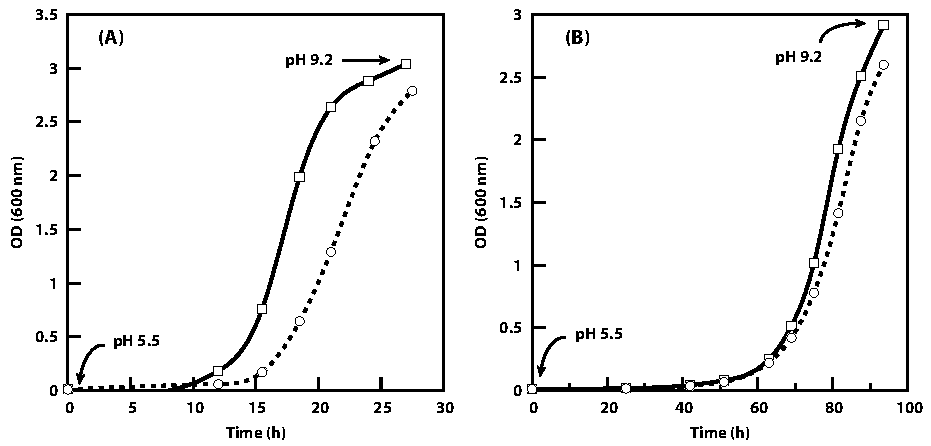
\includegraphics{figures/chap6_ph5}
\end{narrow}
\caption[Growth comparison at pH 5.5]{Growth comparison of
wild-type Lz4W ($\square$) and MbLz4W ($\medcirc$) at pH 5.5 at
22\dg{} (\textbf{A}) and 4\dg{} (\textbf{B}) in unbuffered ABM\@.
pH of the medium and the beginning (adjusted to pH 5.5) and the
end (at stationary phase, pH $\sim$9.2) of the growth are marked
with arrows. Note, the cultures become alkaline with the
progression through growth phases. The X-axis is time in hours and
the Y-axis is the turbidity of the culture, measured as optical
density (OD) at \U{600}{nm}. The culture was diluted five times
for each time point, and the measured OD, to the second decimal,
is multiplied with five, before plotting.}
\label{chap6:growth_low_ph}
\end{figure}

The steady-state growth at low pH was compared, by monitoring the
turbidity of the cultures at \U{600}{nM}. The experiments were
carried out in unbuffered rich medium (ABM), and the pH of the
medium was adjusted to 5.5 by addition of appropriate quantity of
HCl, before inoculation of the bacterial strains. It was observed
that the pH of the culture supernatant were 9.2 both for Lz4W and
MBLz4W at the completion of growth, indicating that the culture
turned alkaline during progression through growth phases.

At 22\dg{}, there was marginal increase in the duration of
lag-phase: \U{$\sim$15}{h} for MBLz4W; \U{$\sim$11}{h} for WT Lz4W
(Figure~\ref{chap6:growth_low_ph}A)\@. These values were higher
than that of the cultures growing at the same temperatures, but
under physiological pH (7.2), where as shown in
Figure~\ref{chap6:mutant_cold_growth}, both these strains reached
OD\sub{600} 0.5 at around \U{11}{h}. Apparently, growth at low pH
could prolong the lag-phase of both these strains.

In log-phase at 22\dg{}, MBLz4W grew slower than Lz4W\@. The slope
of the linear region of the curve in MBLz4W was around 68\% of the
slope observed for Lz4W (Figure~\ref{chap6:growth_low_ph}A).
MBLz4W was thus, about $\sim$30\% slow grower at pH 5.5 and at
22\dg{}\@ than Lz4W growing under same conditions.

At 4\dg{} and pH 5.5, both MBLz4W and Lz4W grew slower than the
cells grown at 4\dg{} and pH 7.0 (compare
Figure~\ref{chap6:mutant_cold_growth}B with
Figure~\ref{chap6:growth_low_ph}). While both these strains took
\U{$\sim$55}{h} to reach stationary phase when grown at pH 7.0 and
4\dg{}, they took about \U{$\sim$100}{h} to reach stationary-phase
at 4\dg{} and pH 5.5. This slow growth was evident throughout all
growth phases. However, at 4\dg{}/pH 5.5, there was no difference
in the lag-phase of growth between Lz4W and MBLz4W.

%MBLz4W, however, was marginally sensitive to simultaneous cold-
%and acid-stress, as displayed by partial growth-retardation
%(Figure~\ref{chap6:growth_low_ph}B). The difference of growth rate
% was almost identical to the difference when the same strains
%were grown at pH 7.0. At log-phase of growth, MBLz4W grew at
%around 83\% of the rate of Lz4W, as calculated from the difference
%of the slopes of the linear region of the two curves in
%Figure~\ref{chap6:growth_low_ph}B\@. Recall, MbLz4W grew at 90\%
%of the rate of Lz4W at physiological pH, at 4\dg{}\@.
%
%It can, therefore, be inferred that Lz4W is more acid-resistant
%during growth at 4\dg{} than while growing at 22\dg{}\@.
%Cold-growth associated resistance also makes these culture acid
%resistant, and this resistance is independent of \emph{rpoS}.
%MBLz4W, however, grew about two third of the rate of Lz4W at room
%temperature and at pH 5.5 in \emph{rpoS}-dependant manner. This
%further consolidates our earlier conclusion that the truncated
%$\sigma$\su{S} is indeed functional in Lz4W and in addition to its
%role in stationary-phase, it plays a important role during
%logarithmic growth of the cells.

A closure look revealed  that MBLz4W was relatively more
acid-resistant at 4\dg{} than the cells growing at 22\dg{}
(Figure~\ref{chap6:growth_low_ph}B). This ability was further
tested at extreme low pH (4.5). When MBLz4W and Lz4W were compared
for their growth capabilities at pH 4.5 and 4\dg{}, there was a
complete growth inhibition of MBLz4W (Figure~\ref{chap6:ph_4_5}).
For Lz4W, there was an extremely long lag-phase ($\sim$13 days),
but the growth rate at log-phase was not altered. The culture pH
was also became alkaline at stationary-phase. MBLz4W, on the other
hand, did not grow at all and the culture pH remained acidic.

\begin{figure}[tbp]
\centering
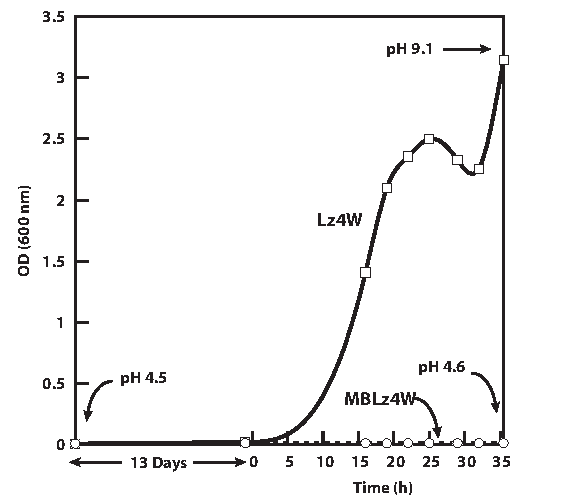
\includegraphics{figures/chap6_ph4_5}
\caption[Growth comparison at pH 4.5]{Growth comparison of Lz4W
($\square$) and MBLz4W ($\medcirc$) at pH 4.5 and 4\dg{}\@. Time
(h) in X-axis plotted against turbidity of the culture, measured
as optical density (OD) at \U{600}{nm}, in Y-axis. Note the
initial lag period of 13 days for Lz4W and the complete growth
retardation of MBLz4W. The measured pH of the culture supernatant
is indicated with arrows.} \label{chap6:ph_4_5}
\end{figure}

Putting together, the results are indicative of the role of
\emph{rpoS} during growth at extreme low pH, in cold. Furthermore,
as shown by the extremely prolonged lag-phase, the \emph{rpoS}
might play a crucial role during acclimatization of cells for
growth in such extreme conditions.

\subsection{Studies on catalase-peroxidase activity}

\emph{rpoS} is known to be involved in modulating the expression
of genes that play a role in defence against oxidative stress.
Keeping this information in mind, a detailed study on the catalase
activity Lz4W cells was carried out. Specific activities of
catalase were measured in crude extract of cell samples collected
from various phases during growth at 22\dg{} and at 4\dg{}
(Figure~\ref{chap6:catalase}A)\@. The crude cell extracts were
prepared as described in Section~\ref{crude} on
page~\pageref{crude}, and the catalase specific activity in these
extracts were measured using the method described in
Section~\ref{chap2:spec_catalase} on
page~\pageref{chap2:spec_catalase}.


\begin{figure}[tbp]
\centering
\includegraphics{figures/chap6_catalase}
\caption[Studies on catalase of Lz4W]{Studies on catalase of Lz4W.
\textbf{(A)} Growth curves of wild-type Lz4W (solid line) and
MBLz4W (dotted line) at 22\dg{} and at 4\dg{}\@. The growth phases
of sample collection are indicated by arrows. \textbf{(B)} The
catalase specific activities at 22\dg{} and 4\dg{} of samples
collected at OD\subsf{600} 0.5, 1.0, 1.5. The data plotted are the
averages of measured catalase activities of three independent
cultures. \textbf{(C)} Catalase isozyme of Lz4W detected with
activity staining in native polyacrylamide gel, in crude extract
from cells growing at 22\dg{} collected at OD\subsf{600} 0.5, 1.0,
and 1.5. The lane number indicated below and the OD\subsf{600} of
the cells are indicated on top. \textbf{(D)} Catalase isozyme of
MBLz4W detected in native polyacrylamide gel, in crude extract
from cell samples collected at OD\subsf{600} 0.5, 1.0, and 1.5.
The lane numbers and the OD of the samples are indicated as (C).}
\label{chap6:catalase}
\end{figure}

It was observed that Lz4W expresses catalase activity in growth
phase dependent manner (Figure~\ref{chap6:catalase}B)\@. During
growth at 22\dg{} ($\square$, in Figure~\ref{chap6:catalase}B) the
activity of catalase increased with the progression of the growth
phase. The activity increased from 36 units at mid-log phase
(OD\sub{600} $\sim$0.5) to $\sim$42 at late-log phase (OD\sub{600}
$\sim$1) and maximum activity was $\sim$49 at early stationary
phase (OD\sub{600} $\sim$1.5). At 4\dg{} ($\blacksquare$, in
Figure~\ref{chap6:catalase}B), however, the activity showed a
marginal decrease with the growth. The maximum activity was
observed during mid-log phase (OD\sub{600} $\sim$0.5) where the
activity was $\sim$26 units. The activity decreased with the
progression through growth phases. It was $\sim$24 and $\sim$20
units in cells at OD\sub{600} $\sim$1.0 and $\sim$1.5,
respectively.

As described in Section~\ref{chap6:rpos_expression}, during growth
at 4\dg{}, the RpoS level increases at the entry of the stationary
phase. A decrease in the catalase level at stationary phase during
growth at 4\dg{}, therefore, indicates that \emph{rpoS} is not
involved in the catalase expression in Lz4W.

In MBLz4W, however, there was an increase in the catalase
activity, both at low and high temperatures, when compared with
wild-type Lz4W (Figure~\ref{chap6:catalase}B)\@. At 22\dg{}
($\medcirc$, in Figure~\ref{chap6:catalase}B), catalase activity
was highest during mid-log phase ($\sim$75 units). The activity
decreased with progression of growth: $\sim$44 units at late-log
and $\sim$47 units at the early stationary phase. At 4\dg{}
($\medbullet$, in Figure~\ref{chap6:catalase}B), the activity,
although lower than in cells grown at 22\dg{}, was still highest
at mid-log phase, with $\sim$43 units. The activity decreased with
the progression of growth: $\sim$31 units at late-log and $\sim$30
units at early stationary phase.

The increase of catalase activity in MBLz4W was reminiscent of the
expression profile of HPI activity in \bact{Ec}, described in
\citet{Visick1997}. HPI, though earlier reported to be \emph{rpoS}
controlled~\citep{Ivanova1994}, was later shown to be upregulated
in \emph{rpoS} mutant~\citep{Visick1997}. The result reported here
for \e{P. syringae} Lz4W was, thus found to be similar to the HPI
activity in \bact{Ec}

In an effort to identify the isozymes of catalase, if any, in
Lz4W, activity staining in native polyacrylamide gel was carried
out as described in Section~\ref{chap2:activity_staining} on
page~\pageref{chap2:activity_staining}. Only one isozyme of
catalase was detected in Lz4W (Figure~\ref{chap6:catalase}C). The
band intensity increased with the progression through the growth
phases. The activity staining profile shown in
Figure~\ref{chap6:catalase} was a representative observed with
crude extract isolated from cells grown at 22\dg{}\@. The result,
therefore, corroborated the earlier measurement of specific
activity the catalase in cells grown at 22\dg{}\@. The activity
staining of the catalase in cell extract from MBLz4W
(Figure~\ref{chap6:catalase}D) also detected only one isozyme of
catalase. The expression profile in native gel, too, conformed
with the specific activity, measured earlier.

Overall, it can be inferred that there is possibly only one
isozyme of catalase present in Lz4W. Although, the expression of
this catalase at stationary phase in the room temperature grown
cells was higher than the expression detected during mid-log
phase, the increase was most probably not due to \emph{rpoS}. This
conclusion was based on the fact that during cold-growth, the
expression of catalase decreased at stationary phase, when there
was an increase in the RpoS level, measured by immunoblot
analysis. Although, the decrease was maintained in the \emph{rpoS}
null-mutant during cold-growth, the expression profile in MBLz4W
at 22\dg{} was completely opposite to the wild-type Lz4W at the
same temperature. The catalase activity was also increased in the
\emph{rpoS} mutant, indicating that a compensatory mechanism is
probably at work. This increase of activity was also highest in
the cells at mid-log phase where the activity was doubled in
mutant compared with wild-type cells.

\subsection{Construction and expression of chimeric full-length \emph{rpoS}}

As shown earlier, amber mutation in \lzsig{} results in a
truncated $\sigmaup$\su{S} (Figure~\ref{chap6_rpos_western}).
There was no indication that this amber might be suppressed by
amber-suppression or even by a read-through, as no cross reacting
band \U{>31}{kDa} was observed in immunoblot analysis.


To inquire the role of this amber mutation in \emph{rpoS}
activity, it was essential to create a full-length RpoS without
the amber, but otherwise similar in all aspects. Because, the
C-terminal half of \pasig{} from \bact{Pa} was almost identical to
the \lzsig{} and there was a suitable \emph{Bam}HI site for
cloning, it was decided that the C-terminal end of the RpoS
(\emph{BamHI}--\emph{Pst}I) on insert in plasmid p4C12 containing
\lzsig{} would be replaced with the C-terminal
(\emph{Bam}HI--\emph{Hin}dIII) fragment from plasmid pDB18R
containing, \pasig{}\@. As shown in Figure~\ref{chap6:swap}, the
exchanged region, following the \emph{Bam}HI site, would create
very little difference in the primary sequence of the protein. All
the variations in the resulting chimeric RpoS (RpoS$\chiup$)  are
summarized in Table~\ref{chap6:rpos_chi_changes}. There would be
only one non-conserved change, L298Q, in \lzsig{}. As this change
is after the amber mutation, its effect was inconsequential. There
would be only two changes before the amber, Q192H and S225T\@. As
these changes are very strongly conserved, it was presumed that
they would have little, if any, effect on the the function of
RrpoS$\chiup$ in the bacterium. \emph{rpoS}$\chiup$ would,
therefore, be very similar to \lzsig{} in all aspects, but
without the amber mutation.

\begin{sidewaysfigure}[tbp]
\centering
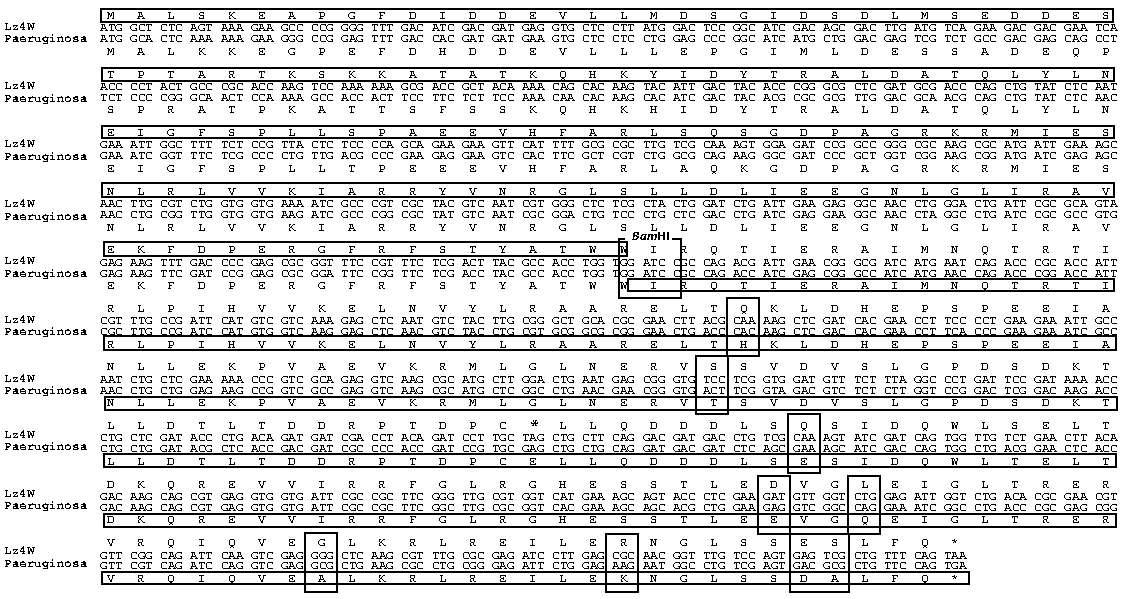
\includegraphics{figures/chap6_fusion_codon}
\caption[Domain swapping of Lz4W \emph{rpoS}]{Swapping of
C-terminal half between \emph{rpoS}\subsf{Lz4W} and
\emph{rpoS}\subsf{Pa}. The reading-frame of
\emph{rpoS}\subsf{Lz4W} and \emph{rpoS}\subsf{Pa} are aligned. The
amino acids are indicated on top of the codons for
\emph{rpoS}\subsf{Lz4W} and below codons for
\emph{rpoS}\subsf{Pa}. The amino acid sequence of the resulting
protein is indicated by the horizontal box. The \emph{Bam}HI site
(the site of exchange) is marked with a box and the amber mutation
in \emph{rpoS}\subsf{Lz4W} is marked with $\ast$. Each change of
the amino acid sequence in the resulting protein is marked with
vertical box.} \label{chap6:swap}
\end{sidewaysfigure}

\begin{table}[tbp]
\begin{minipage}[c]{\textwidth}
\renewcommand{\footnoterule}{}
\caption[Amino acid change in \emph{rpoS}$\chiup$ ]{Amino acid
changes in \emph{rpoS}$\chiup$} \label{chap6:rpos_chi_changes}
\begin{narrow}{-1in}{-1in}
\centering
\begin{small}
\begin{tabular}{p{1.5in}p{1.5in}p{1.5in}}\toprule
\textbf{Position} & \textbf{Change} & \textbf{Type of
change}\protect\footnote{Conserved and non-conserved designation
as determined by Gonnet Pam250 matrix. Strong conserved
designation denote score >0.5.}
\\\midrule\addlinespace
\multicolumn{3}{l}{\textbf{Before amber}}\\
192 & Q $\rightarrow$ H & Strongly Conserved \\
225 & S $\rightarrow$ T & Strongly Conserved \\\addlinespace
\multicolumn{3}{l}{\textbf{After amber}} \\
262 & Q $\rightarrow$ E & Strongly Conserved\\
295 & D $\rightarrow$ E & Strongly Conserved \\
298 & L $\rightarrow$ Q & Not conserved\\
314 & G $\rightarrow$ A & Conserved \\
324 & R $\rightarrow$ K & Strongly conserved\\
330 & E $\rightarrow$ D & Strongly conserved\\
331 & S $\rightarrow$ A & Strongly conserved\\
\bottomrule
\end{tabular}
\end{small}
\end{narrow}
\end{minipage}
\end{table}

The plasmid pXRPOS containing \emph{rpoS}$\chiup$ was constructed
by ligating N-terminal \emph{Pst}I--\emph{Bam}HI DNA fragment from
plasmid p4C12 containing \lzsig{} and the C-terminal
\emph{Bam}HI--\emph{Hin}dIII DNA fragment from plasmid pDB18R,
containing \pasig{}, on a broad-host-range plasmid
pGL10~\citep[Figure~\ref{chap6:pxrpos}E]{Bidle1999}. The over-all
scheme of the construction is shown in Figure~\ref{chap6:pxrpos}.
In pXRPOS, the reading frame of \emph{rpos}$\chiup$ was in the
opposite orientation to that of the \emph{lacZ} promoter of the
vector. Thus, the expression of the chimeric gene from pXRPOS, was
expected to be solely driven by the promoter of \lzsig{}.

\begin{sidewaysfigure}[tbp]
\centering
\includegraphics{figures/chap6_pxrpos}
\caption[Construction of pXRPOS]{Construction of plasmid pXRPOS,
containing chimeric, full-length \emph{rpoS}, \emph{rpoS}$\chiup$.
The C-terminal \emph{Bam}HI--\emph{Hin}dIII fragment (C) from
plasmid pDB18R (A) and N-terminal \emph{Pst}I--\emph{Bam}HI
fragment (D) from p4C12 (B) were cloned into plasmid pGL10 (E), in
a three-way ligation. The resulting plasmid, designated pXRPOS
(F), contained the chimeric \emph{rpoS} where the promoter and
N-terminal half of the gene was from Lz4W \emph{rpoS} and the
C-terminal half was derived from \bact{Pa} \emph{rpoS}. Note, in
pXRPOS, the chimeric gene was cloned in the opposite orientation
to that of \emph{LacZ} promoter of the vector.}
\label{chap6:pxrpos}
\end{sidewaysfigure}

When transformed in the null-mutant MBLz4W, pXRPOS indeed produced
a full-length RpoS protein (Figure~\ref{chap6:pxrpos_expression}).
Three independent transformed clones (lanes 1, 2, 3 in
Figure~\ref{chap6:pxrpos_expression}) were tested for the presence
of RpoS protein by immunoblot analysis. All of them exhibited the
presence of a positive band of size \U{$\sim$45}{kDa}. As it was
demonstrated earlier, MBLz4W was negative for RpoS protein on
immunoblot (Figure~\ref{chap6:mutant_southern}A), and the
cross-reacting band in Lz4W was of size \U{$\sim$31}{kDa}. RpoS in
\bact{Ec}, and \bact{Pa} is also known to migrate as
\U{41--45}{kDa} band on SDS-PAGE. It was, thus, confirmed that
\emph{rpoS}$\chiup$ on pXRPOS indeed could produce a full-length
\sigs{} in Lz4W.

\begin{figure}[tbp]
\centering
\includegraphics{figures/chap6_pxrpos_western}
\caption[Full-length \emph{rpoS} expression from
pXRPOS]{Full-length \emph{rpoS} expression from pXRPOS. Three
independent clones (lanes 1, 2 and 3) of MBLz4W, transformed with
plasmid pXRPOS was tested for the expression of RpoS in
immunoblot. Cell cultures collected at the stationary phase were
lysed directly in SDS-PAGE loading buffer and tested using
anti-RpoS antibody, as described in Section~\ref{mat:immunoblot}.
The positive band of RpoS is marked with as arrow. The molecular
weight markers are indicated on the right.}
\label{chap6:pxrpos_expression}
\end{figure}

\subsection{\emph{rpoS}$\chiup$ causes cold-sensitivity in MBLz4W}
\label{cold_sensitivity}

The effect of chimeric full-length RrpoS$\chiup$ on the growth
properties of \e{P. syringae} strains were examined in comparison
with the \lzsig{} containing the amber. Both these genes were
supplied in \emph{trans} on the same vector (pGL10). To get rid of
any effect due to the background expression of indigenous
\emph{rpoS}, the experiments were performed in MBLz4W, where the
genomic copy of the \emph{rpoS} has been disrupted. The MBLz4W was
transformed with pXRPOS, carrying the full-length chimeric
\emph{rpoS}$\chiup$, pGLSIGS, carrying the \lzsig{}. The pGLSIGS
was constructed by cloning the \emph{Pst}I insert from plasmid
p4C12 in pGL10. MBLz4W transformed with pGL10, was taken as
plasmid control.

All these strains were identical in their growth properties at
22\dg{} when grown in ABM broth (Figure~\ref{chi_growth}A).
Introduction of the plasmid, however, prolonged the time for
growth completion to \U{36}{h} from the usual \U{24}{h}.

Interestingly, at 4\dg{}, pXRPOS caused severe growth retardation
(Figure~\ref{chi_growth}B). The growth defect was prominent in
both lag-phase as well as in the log-phase. MBLz4W containing
empty plasmid vector grew fastest, while MBLz4W containing pGLSIGS
grew with an intermediate rate. MBLz4W, carrying pXRPOS took the
longest time to grow, and reached a maximum turbidity lesser than
the other two strains.

At exponential phase, MBLz4W (pXRPOS) was about 45\% slow grower,
compared with MBLz4W (pGL10), as measured by the difference of the
slope of the linear region of the growth curve shown in
Figure~\ref{chi_growth}B\@. MBLz4W (pGLSIGS) on the other hand,
was only 10\% slow grower than MBLz4W carrying pGL10.

\begin{figure}[tbp]
\begin{narrow}{-1in}{-1in}
\centering
\includegraphics{figures/chap6_chimera_growth}
\end{narrow}
\caption[Growth properties of MBLz4W]{Growth comparison of MBLz4W,
transformed with pXRPOS ($\triangle$), containing chimeric
\emph{rpoS}$\chiup$, with pGLSIGS ($\medcirc$), containing
\emph{rpoS}\subsf{Lz4W}, with pGL10 ($\square$), at 22\dg{} (A)
and at 4\dg{} (B). The turbidity of the cultures measured as
optical density (OD) at \U{600}{nm} in Y-axis plotted against time
in hours at X-axis.} \label{chi_growth}
\end{figure}

Based on this result, it can be proposed that the amber, present
in the \lzsig{} reading frame, might actually confer an advantage
during exponential phase of growth at low temperature in the
wild-type Lz4W. It was shown earlier in this study, that MBLz4W
was about 10\% slow grower than the wild-type Lz4W at 4\dg{}. When
supplied in \emph{trans}, neither \lzsig{}, nor the full-length
chimeric \emph{rpoS}$\chiup$ rescued the phenotype. Instead, both
these alleles of \emph{rpoS} actually aggravated the
cold-sensitivity of MBLz4W. This can only be explained by the
assumption that the expression of plasmid borne \emph{rpoS} might
be more than the genomic copy, and this higher expression might be
responsible for the aggravated cold-sensitivity of MBLz4W. Higher
expression of RpoS is, therefore, detrimental for Lz4W during
growth at low temperature. The downregulation of RpoS expression
during cold growth, shown in Section~\ref{chap6:rpos_expression},
further supports this hypothesis.

\subsection{pXRPOS increases viability of Lz4W at stationary phase}

As shown earlier, the expression of a full-length \emph{rpoS} in
\emph{trans} caused growth retardation at 4\dg{}. In an attempt to
find whether the chimeric full-length \emph{rpoS} has any effect
other than the growth retardation at low temperature, the
survivability of MBLz4W carrying pXRPOS, pGLSIGS, and PGL10 were
tested at stationary phase during growth at 4\dg{}. Aliquots of
culture, after serial dilution were plated every \U{24}{h},
beginning with the \U{6}{h} after completion of the growth
(OD\sub{600} $\sim$3), for six days (Figure~\ref{chap6:death}).
The viability of the cells was measured as colony forming units
(CFU) per ml of the culture.

\begin{figure}[tbp]
\includegraphics{figures/chap6_death}
\caption[Viability comparison of MBLz4W]{Viability of MBLz4W at
stationary phase during growth at 4\dg{}, when transformed with
pXRPOS ($\triangle$), pGLSIGS ($\medcirc$) and pGL10 ($\square$).
Viability measured as colony forming units (CFU) per ml of culture
in Y-axis is plotted against Days in X-axis. Note the
post-stationary steep viability-loss upto three days.}
\label{chap6:death}
\end{figure}

pXRPOS was found to increase  the viability of MBLz4W, compared to
the plasmid control. While there was a sharp decrease in the
viability for all the three cultures for three days after growth
completion, the viability recovered after three days. During the
initial decline, the viability dropped almost five orders of
magnitude for MBLz4W carrying the empty plasmid pGL10 ($\square$,
in Figure~\ref{chap6:death}). During that interval, the viability
loss of MBLz4W (pXRPOS) ($\triangle$) was only ten fold, and loss
was 100 fold for MBLz4W (pGLSIGS) ($\medcirc$).

After post-stationary three days, the viability recovered in all
the three strains. Interestingly, MBLz4W carrying pGLSIGS
(\e{rpoS} carrying amber) recovered to the level of the MBLz4W
carrying the full length chimeric \emph{rpoS}. At the end of the
six days, the net viability-loss for MBLz4W carrying pXRPOS and
pGLSIGS were only ten folds, while for plasmid control it was 1000
folds.

Evidently, \emph{rpoS}$\chiup$, although caused cold-sensitivity
when supplied in \emph{trans}, increased the viability of cells at
stationary phase. A noted effect of \lzsig{} was to allow the
MBLz4W cells to survive at stationary phase almost to the level of
full-length \emph{rpoS}.

\subsection{Expression level of the plasmid borne \emph{rpoS}}

As discussed in Section~\ref{cold_sensitivity}, one of the reasons
for cold sensitivity of the \emph{rpoS}$\chiup$ bearing strains
might be due to a high level of RpoS expression from the plasmid
borne \emph{rpoS}. This hypothesis was tested by directly
comparing RpoS protein levels in cells, bearing plasmid borne
\emph{rpoS}, in semi-quantitative immunoblot analysis
(Figure~\ref{chi_expression}). The RpoS protein levels were
markedly higher in cells bearing plasmid encoded RpoS, than the
strains containing only the genomic copy
(Figure~\ref{chi_expression}D)\@. Interestingly, plasmid encoded
\lzsig{} expression was lower than the plasmid encoded
\emph{rpoS}$\chiup$ (Figure~\ref{chi_expression}C), although both
were on the same plasmid (pGL10). At OD\sub{600} 0.5, the
expression of \lzsig{} was 20 folds lesser than
\emph{rpoS}$\chiup$, when supplied in \e{trans} on plasmid. With
the progression through growth phases the difference in the level
of expression decreased about 10 folds at OD\sub{600} 1.0 and
about 4 folds at OD\sub{600} 1.5.

\begin{figure}[tbp]
\begin{narrow}{-1.5in}{-1.5in}
\centering
\includegraphics{figures/chap6_chi_expression}
\end{narrow}
\caption[Comparison of plasmid borne RpoS levels]{Comparison of
RpoS levels of MBLz4W, when transformed with pXRPOS, carrying
chimeric full-length \emph{rpoS}$\chiup$, pGLSIGS, carrying
\lzsig{} and the wild type Lz4W. \textbf{(A)} Immunoblot showing
the RpoS levels at 22\dg{} in cells, collected at OD\subsf{600}
0.5, 1.0 and 1.5. OD\subsf{600} of each sample is marked on top of
each lanes and the lane numbers are indicated below. The major
RpoS bands are marked with arrows. For comparison with the genomic
level of RpoS, Lz4W wild type cells of OD\subsf{600} 1.5 loaded in
lane 7. Lanes 1--3, MBLz4W, transformed with pGLSIGS; lanes 4--6,
MBLz4W, transformed with pXRPOS. \textbf{(B)} Ponceau S stained
blot showing equal loading. \textbf{(C)} Comparison of the RpoS
level between MBLz4W, transformed with pXRPOS (open bar) and
MBLz4W, transformed with pGLSIG (black bar), measured as intensity
of the RpoS band. \textbf{(D)} Comparison of the levels of RpoS
coded by genomic copy of \emph{rpoS} in wild type Lz4W (hatched
bar) with the plasmid encoded RpoS in MBLz4W, carrying
\emph{rpoS}$\chiup$ (open bar) and in MBLz4W, carrying pGLSIGS
(black bar).} \label{chi_expression}
\end{figure}


When compared with the level of expression from the genomic copy
of \emph{rpoS}, both the plasmid encoded genes showed markedly
higher expressions (Figure~\ref{chi_expression}D)\@. At
OD\sub{600} 1.5, plasmid coded \lzsig{} showed 3 folds more
expression than expression from the genomic copy. The expression
of \emph{rpoS}$\chiup$ from plasmid  was almost 12 times more than
the expression from the genomic copy. The production of RpoS was
expectedly higher when expressed from the plasmid. The unusual
high amount of RpoS produced from the plasmid encoded
\emph{rpoS}$\chiup$ is surprising. A possible explanation could be
in the difference in proteolytic degradation of the two different
types of RpoS, one being intact protein, and the other being
truncated.

\section{Discussion}

\emph{rpoS} is the master regulator of general stress response in
Gram negative bacteria~\citep{Hengge2002}. In spite of decades of
research, its exact role in each of the stress pathway remains as
elusive as ever. Only very recently, the molecular mechanisms of
regulation of \emph{rpoS} is beginning to emerge. This is not
surprising, given that the expression of \emph{rpoS} is controlled
at every possible means known to occur in cell. The knowledge of
downstream pathway of each of the stress response, however, is
still fragmentary. On one hand, the role of \emph{rpoS} in
oxidative stress response is broadly worked out, on the other hand
its role in cold-stress is, at best, arguable. Several of the
known \emph{rpoS}-controlled promoters in \bact{Ec} have been
shown to be upregulated during growth at low
temperature~\citep{Sledjeski1996,Rajkumari2001}. RpoS expression
itself is upregulated during exponential growth at low
temperature. But \bact{Ec} \emph{rpoS} mutant has no growth defect
at low temperature~\citep{Sledjeski1996}.

The work presented in this study have demonstrated that, in
contrary to findings in \bact{Ec}, Lz4W \emph{rpoS} mutant is
cold-sensitive, albeit marginally. It has also been shown that
Lz4W \emph{rpoS} harbors an amber mutation in its reading-frame,
which results in a truncated, but functionally competent protein,
as judged by the severe acid-sensitivity of the null-mutant. In
contrast to \bact{Ec}, RpoS in Lz4W is downregulated during
cold-growth. Moreover, expression of either the indigenous
\emph{rpoS} (with amber) or a full-length chimeric \emph{rpoS} in
\emph{trans} did not alleviate, rather, aggravate the
cold-sensitivity of the \e{rpoS} null-mutant.


The present study also examined the role of \emph{rpoS} during
exponential growth of Lz4W at low temperature. All the phenotypes
of the \emph{rpoS} null-mutant tested, namely growth in low pH,
low temperature, or both together showed a distinct defect at lag
and exponential growth phase, implicating a role for \emph{rpoS}
in various growth phases of this bacterium. Unfortunately, not
much is known about role of \emph{rpoS} during exponential growth,
neither in mesophiles nor in psychrotrophs. In spite of its low
expression during exponential phase~\citep{Lange1991}, \emph{rpoS}
is known to control at least two genes in \bact{Ec} during
exponential phase: \emph{xthA}~\citep{Sak1989} and
\emph{aidB}~\citep{Loewen1994}. Both these genes were shown to be
involved in repair of DNA damage in \bact{Ec}.

As shown by activity staining, there is only one catalase isozyme
present in \e{P. syringae} Lz4W\@. Although, the the expression of
this catalase is growth phase dependent, it is probably not
\emph{rpoS} dependent, because, during growth at 4\dg{}, the
catalase activity did not increase with the observed increase in
RpoS level. Moreover, the activity was higher in \e{rpoS}
null-mutant. This finding is in the line with the recent
observation that HPI level increases in \bact{Ec} \emph{rpoS}
mutant~\citep{Visick1997}. There was also earlier report that
several \siga{}-controlled gene are expressed more in \sigs{}
mutant~\citep{Farewell1998}.

If \emph{rpoS} is important during growth of the cold-adapted
\e{P. syringae} at low temperature, then why does it harbor an
amber? The answer to this question lies in the discovery of GASP
mutants (see Section~\ref{chap6:intro}). The mechanism is akin to
the selection of cancerous cells in multicellular organism and has
been explained through game theory~\citep{Vulic2001}. GASP alleles
of \emph{rpoS} are believed to be defective in density dependent
growth inhibition, and are believed to grow at the expense of the
wild type cells. One of the postulate of the theory is that GASP
mutants would have selective advantage only in presence of large
excess of wild type cells, a phenomenon described as
\emph{evolutionary cheating}. As will be discussed in the next
chapter, this theory can not explain the wide-spread mutant
alleles of \emph{rpoS} in nature, where in the absence of the wild
type cell, \emph{rpoS} GASP allele would have lost its selective
advantage. A presumptive proposition will be that the mutant
alleles of \emph{rpoS} does indeed confer a hitherto unknown
selective advantage on the cells carrying it.

The first evidence of such an advantage came from a recent work,
where it was shown that under conditions of slow growth in
chemostat culture, \emph{rpoS} mutants could be selected over wild
type cells. Moreover, under condition of dual-stress, most often,
an amber containing \emph{rpoS} gets selected and gets fixed in
the population~\citep{Mcrobb2002}. The authors argued that
upregulation of \emph{rpoD} activity is the cause for the
selection of \emph{rpoS} mutants over the wild type allele. In
situation of dual stress, an attenuated version of \emph{rpoS}
gets selected to deal with the additional stress.

Lowering of one $\sigmaup$ factor does upregulate the activity of
the others; what termed as $\sigmaup$ factor competetion
model~\citep{Farewell1998,Zhou1992}. The phenomenon is based on
the fact that in \bact{Ec}, and probably in other bacteria, the
total number of $\sigmaup$ factors ({$\sim$1200} molecules) is
more than the total number (600--700 molecules) of core enzyme
molecule available to form holoenzyme, at any give
time~\citep{Ishihama2000}.

An amber would be a way to downregulate the RpoS level during
vegetative growth but maintaining enough RpoS activity to cope
with additional stress. There are several ways this might be
achieved. First, a read-through of the amber might produce low but
sufficient RpoS, or second, depending on the position of the amber
a truncated protein might actually results in promoter
discrimination within \emph{rpoS} regulon. An indication of this
was presented in Chapter 5 of this study. How could promoter
discrimination within \emph{rpoS} regulon upregulate other
$\sigmaup$ factors? A potent way would be the regulation by
anti-$\sigmaup$ factors. For example, \emph{rsd}, the regulator of
$\sigmaup$\su{70} in \bact{Ec} was found to be \emph{rpoS}
controlled~\citep{Jishage1999}. A search for \emph{rsd} homolog in
sequenced genomes identified its homolog in all known sequenced
genomes (data not shown). In \bact{Pa}, \emph{algQ} is a potential
anti $\sigmaup$\su{70}. Lastly, a truncated $\sigmaup$ might
possess an altered binding affinity to core RNA polymerase,
thereby, modulating the level of holo RNA polymerase.

In Lz4W, the growth at exponential phase probably involves
vegetative $\sigmaup$ factor. A lowering of the \emph{rpoS} level
would potentially upregulate \emph{rpoD} activity, thereby,
promoting growth. A distinct downregulation of RpoS level was
observed during growth of Lz4W at low temperature, indicating, any
mechanism that might downregulate RpoS could potentially promote
growth at low temperature. It is also to be noted that disruption
of the \emph{rpoS} made Lz4W cold-sensitive, indicating a complete
loss of RpoS function is detrimental for growth at low
temperature. Moreover, expression of \emph{rpoS} in high level
actually made Lz4W severely cold-sensitive. Putting all these
observations together, it is obvious that the amber in the
\emph{rpoS} reading frame is actually an optimum condition, which
might have been selected during growth at low temperature.

Can this phenomenon be extended to other bacteria. There are
contradictory evidences in studies in \bact{Ec}. \emph{rpoS} is
actually upregulated in \bact{Ec} during growth at low
temperature~\citep{Sledjeski1996}. Exogenous expression of ppGpp,
the alarmone, which increases the affinity of the core RNA
polymerase to \sigs{}~\citep{Jishage2002}, makes \bact{Ec}
cold-sensitive~\citep{Jones1992}. More studies are, therefore,
required before the conclusion from the present study can be
extended to other bacteria, in more general sense.\ding{45}

\FloatBarrier\pagebreak \thispagestyle{empty}
\begin{figure}[h]
\raggedleft
\includegraphics{figures/chap7_sep}
\end{figure}
\thispagestyle{empty}

\include{discussion}
\backmatter
\linespread{1}\normalsize

\afterpage{\addcontentsline{toc}{chapter}{Bibliography}}
\lhead{\myline} %\rhead{\myrightheader{\rightmark}}
%\begin{small}
%\bibliography{rpos,rpoh,rpod,pseudo_rpos,thesis}
\bibliography{thesis}
\bibliographystyle{myapalike}
%\bibliographystyle{newbioinfo}
%\end{small}
%\printindex
\linespread{1.1}\normalsize
\chapter{Colophon}

{\scshape This is my first} attempt to try a real big document in
\LaTeX. Failed to digest \textit{Knuth}, I had to swallow
\textit{Lamport}. And I loved it. \LaTeX{} made typing this thesis
a pleasure and in the process I started gnawing a bit on \TeX{}
and hope someday I'll write in it.

The citations are in \textsf{\small apalike} style. I hacked the
original \textsf{\small bst} file to create some modifications
that I wanted. The text font is Adobe Minion and the title font
Adobe Myriad. These type1 fonts were imported into \LaTeX{} by
\textsf{\small fontinst} package. I generated the Bib\TeX{}
\textsf{\small bib} files directly from Pubmed citations by a perl
script that I wrote. The figures are made in Macromedia Freehand
10 and exported as PDF before importing into PDF\TeX. Plasmid maps
are drawn by an web-based application Savvy
({\small\url{http://www.bioinformatics.org/savvy}}) that I wrote
as part of my \textsf{\small BioSVG} project. Maps drawn by Savvy
are in Scalable Vector Graphics (SVG) format. The chromatogram
files are also drawn by my own \textsf{\small ABITrace} perl
module in SVG format. I converted the SVG file to PDF by Apache
project's FOP into PDF before importing them into PDF\TeX{}. All
the plots in this thesis were drawn with GNUPlot, another
marvellous gift from free software community.

The pictures on the chapter separators are illustrations by John
Tenniel in Modern Library's \e{The Complete Works of Lewis
Carroll}.

Lastly, I proudly declare this thesis M\$ Office free. None of
Micro\$oft's bloated and buggy code was used to make any part of
this thesis. At last I did something \emph{unofficial}. \ding{45}



\end{document}
